\documentclass{article}
% Shared preamble for main.tex and supp.tex (X-regularization, arXiv split).
% \input by both documents after their own \documentclass.
\usepackage[letterpaper, margin=1in]{geometry}
\usepackage{setspace}
\usepackage{amsmath,amssymb}
\usepackage{graphicx}
\usepackage{subcaption}
\usepackage[amsmath,thmmarks,framed]{ntheorem}
\usepackage{authblk}
\usepackage{tcolorbox}
\usepackage{booktabs}
\usepackage{multirow}
\usepackage{placeins}
\usepackage{enumerate}
\usepackage{xcolor}
\definecolor{darkgreen}{rgb}{0.0,0.5,0.0}
\usepackage[colorlinks,linkcolor=red,citecolor=darkgreen,urlcolor=blue]{hyperref}
\usepackage{xr-hyper}   % cross-document references between main.tex and supp.tex (must follow hyperref)
\usepackage[round,authoryear]{natbib}

\usepackage[ruled,linesnumbered]{algorithm2e}
\SetKwInput{KwInput}{Input}
\SetKwInput{KwOutput}{Output}

\newtheorem*{remark}{Remark}
\newtheorem{lemma}{Lemma}
\newtheorem{theorem}{Theorem}
\newenvironment{proof}{\par\medskip\noindent\textit{Proof.}\ }{\hfill$\square$\par\medskip}

\newcommand{\Le}{\leqslant}
\newcommand{\Ge}{\geqslant}
\newcommand{\D}{\mathrm{d}}
\newcommand{\KL}{\mathrm{KL}}
\newcommand{\X}{\mathrm{X}}
\newcommand{\ESS}{\mathrm{ESS}}

\theoremstyle{plain}

\externaldocument[M-]{main}   % resolve (1), Figure 1, Theorem 1, Section 3 -> main.tex

% --- Supplement numbering: S-prefixed sections / equations / floats / theorems ---
\renewcommand{\thesection}{S\arabic{section}}
\renewcommand{\theequation}{S\arabic{equation}}
\renewcommand{\thefigure}{S\arabic{figure}}
\renewcommand{\thetable}{S\arabic{table}}
\renewcommand{\thetheorem}{S\arabic{theorem}}
\renewcommand{\thelemma}{S\arabic{lemma}}

\title{Supplementary Material\\[2pt] Forward KL Can Be Better: Normalizing Flow Boltzmann Sampling with X-Regularization}
\author[1]{Qi Feng}
\author[2]{Rongjie Lai}
\author[2]{Di Qi}
\author[2]{Xuda Ye}
\affil[1]{Department of Mathematics, Florida State University, Tallahassee, FL 32306}
\affil[2]{Department of Mathematics, Purdue University, West Lafayette, IN 47907}
\date{\today}

\begin{document}
\maketitle

\noindent This supplement collects the full derivations and experiments abridged in the main text: the Fisher--Rao gradient-flow analysis (Section~\ref{sec: FR}), the model-problem study (Section~\ref{sec: experiments}), and the molecular potential-energy experiments (Section~\ref{sec: molecular}). Cross-references of the form (1), Figure~1, Theorem~1, Section~3 point to the main text; those of the form (S1), Figure~S1 are internal to this supplement.

% ===================== Section S1: Fisher--Rao (verbatim main S2) =====================
\section{Fisher--Rao gradient flow with X functionals}
\label{sec: FR}

Before turning to the training algorithm, we study the gradient-flow properties of the loss on the space of densities; the convergence rate of this continuous-time idealization is a proxy for how trainable the corresponding discrete loss is in practice. We view $\nu$ as a generic probability density evolving along the gradient flow of the loss under an appropriate Riemannian metric on the space of densities \citep{ambrosio2008gradient,villani2009optimal} and ask how fast $\nu_t$ converges to the target $\mu$ in $\KL(\mu\|\nu_t)$.

In this section we restrict to the loss with only the forward KL and the shape regularizer $\X_\mu$,
\begin{equation}
    \mathcal L[\nu] = \KL(\mu\|\nu) + \lambda  \X_\mu(\mu\|\nu) = \int_{\mathbb R^d} \mu(x) \log \frac{\mu(x)}{\nu(x)} \D x +
    \lambda\iint_{\mathbb R^d\times\mathbb R^d}
     \mu(x)\mu(y) \biggl|\log\frac{\mu(x)}{\nu(x)} - \log\frac{\mu(y)}{\nu(y)}\biggr| \D x \D y,
    \label{eq: loss KL X}
\end{equation}
where $\lambda>0$ is a fixed constant.
Throughout this section we abbreviate the importance weight by
\begin{equation*}
    w(x) := \frac{\mu(x)}{\nu(x)},
\end{equation*}
so that the log-ratio is $z(x) = \log w(x) = \log\mu(x) - \log\nu(x)$, the field $z$ of \eqref{M-eq: logratio-z}. The importance weight $w$ is distinct from the localization measure $\omega$ in $\X_\omega$.

The choice of Riemannian metric matters. In the Wasserstein-2 geometry, induced by optimal transport \citep{jordan1998variational,otto2001geometry}, the forward KL fails to be displacement convex along Wasserstein-2 geodesics, and the standard Otto--Villani / Bakry--{\'E}mery machinery \citep{otto2000generalization,bakry2014analysis} that yields exponential convergence for the reverse KL does not apply. We therefore work in the Fisher--Rao (FR) geometry \citep{amari2016information,bauer2016uniqueness}, in which the forward KL admits an unconditional exponential decay rate and the regularizer $\X_\mu$ contributes a qualitatively new, nonlocal birth--death modulation \citep{lu2019accelerating}: the local update at $x$ is driven by how the importance weight at $x$ ranks against the population of weights under $\mu$.

Denoting the $\nu$-mean by $\langle \cdot \rangle_\nu := \int( \cdot ) \nu \D x$, the Fisher--Rao gradient of a functional $\mathcal F[\nu]$ and the associated dissipation identity along the FR gradient flow $\partial_t\nu_t = -\mathrm{grad}^{\mathrm{FR}}\mathcal F(\nu_t)$ are
\begin{equation}
    \mathrm{grad}^{\mathrm{FR}}\mathcal F(\nu) = \nu\biggl(\frac{\delta\mathcal F}{\delta\nu} - \Big\langle\frac{\delta\mathcal F}{\delta\nu}\Big\rangle_\nu\biggr),
    \qquad
    \frac{\D}{\D t}\mathcal F[\nu_t] = -\!\int_{\mathbb R^d}\biggl(\frac{\delta\mathcal F}{\delta\nu} - \Big\langle\frac{\delta\mathcal F}{\delta\nu}\Big\rangle_{\nu_t}\biggr)^{2}\nu_t \D x.
    \label{eq: FR-gradient}
\end{equation}
The mean-subtraction enforces $\int\mathrm{grad}^{\mathrm{FR}}\mathcal F = 0$, so the FR flow conserves probability mass.

\subsection{Derivation of $\X_\mu$-regularized Fisher--Rao gradient flow}
\label{subsec: FR-grad-calc}

The first variation of the forward KL with respect to $\nu$ admits the form
\begin{equation}
    \frac{\delta \KL(\mu\|\nu)}{\delta \nu}(x) = -\frac{\mu(x)}{\nu(x)} = -w(x),
    \label{eq: var-KL}
\end{equation}
so by \eqref{eq: FR-gradient}, using $\langle w \rangle_\nu = \int_{\mathbb R^d} \mu \,\D x = 1$, the FR gradient of the forward KL is
\begin{equation}
    \mathrm{grad}^{\mathrm{FR}}\big[\KL(\mu\|\nu)\big](x) = \nu(x) - \mu(x).
    \label{eq: FR-grad-KL}
\end{equation}

For the $\X_\mu$ functional, the inner log-ratio difference has first variation
\begin{equation*}
    \frac{\delta\bigl(\log w(x) - \log w(y)\bigr)}{\delta\nu(x)} = \frac{1}{\nu(y)}\delta(x-y) - \frac{1}{\nu(x)}.
\end{equation*}
By the symmetry of $\X_\mu$ in $x$ and $y$,
\begin{align*}
    \frac{\delta \X_\mu(\mu\|\nu)}{\delta \nu}(x) & =
    2 \int_{\mathbb R^d} \mu(x) \mu(y) \operatorname{sgn}(w(x) - w(y)) \frac{\delta (\log w(x) - \log w(y))}{\delta\nu(x)} \D y \\
    & = 2 \int_{\mathbb R^d} \mu(x) \mu(y) \operatorname{sgn}(w(x) - w(y))
    \bigg(\frac1{\nu(y)}\delta(x-y) - \frac1{\nu(x)}\bigg) \D y \\
    & = -2 w(x) \int_{\mathbb R^d} \mu(y) \operatorname{sgn}(w(x) - w(y))  \D y,
\end{align*}
where the contribution of $\delta(x-y)$ vanishes because $\operatorname{sgn}(w(x) - w(y)) = 0$ at $y = x$. Hence
\begin{equation}
    \frac{\delta \X_\mu(\mu\|\nu)}{\delta \nu}(x) = - 2w(x)S(x),
    \qquad
    S(x) := \mathbb E_{y\sim\mu}\bigl[\operatorname{sgn}(w(x) - w(y))\bigr].
    \label{eq: var-X}
\end{equation}
We call $S$ the \emph{rank field} of the importance weight under $\mu$: $S(x) > 0$ where $w(x)$ exceeds the $\mu$-median of $w$, i.e.\ where $\nu$ undercovers a mode of $\mu$; $S(x) < 0$ where $\nu$ overcovers; and $S \equiv 0$ at $\nu = \mu$. By antisymmetry,
\begin{equation*}
    \mathbb E_\mu[S] = \mathbb E_{x,y\sim \mu}\bigl[\operatorname{sgn}(w(x) - w(y))\bigr] = 0,
\end{equation*}
and the FR gradient of $\X_\mu$ with respect to $\nu$ is
\begin{equation}
    \mathrm{grad}^{\mathrm{FR}}\big[\X_\mu(\mu\|\nu)\big](x) = -2\mu(x) S(x).
    \label{eq: FR-grad-X}
\end{equation}

Since the FR gradient is linear in the functional, the FR gradient of $\mathcal L[\nu] = \KL(\mu\|\nu) + \lambda \X_\mu(\mu\|\nu)$ is the direct sum of \eqref{eq: FR-grad-KL} and \eqref{eq: FR-grad-X}:
\begin{equation*}
    \mathrm{grad}^{\mathrm{FR}}[\mathcal L](x) = \nu(x) - \mu(x) - 2\lambda \mu(x) S(x).
\end{equation*}
The regularized Fisher--Rao gradient flow $\partial_t\nu_t = -\mathrm{grad}^{\mathrm{FR}}[\mathcal L]$ therefore reads
\begin{equation}
    \partial_t\nu_t(x) = \mu(x) - \nu(x) + 2\lambda \mu(x) S_t(x), \quad 
    \text{where~}
    S_t(x) := \mathbb E_{y\sim\mu}\biggl[\operatorname{sgn}\biggl(\frac{\mu(x)}{\nu_t(x)} - \frac{\mu(y)}{\nu_t(y)}\biggr)\biggr].
    \label{eq: FR-L-flow}
\end{equation}
Equation~\eqref{eq: FR-L-flow} is a \emph{nonlocal} PDE: its right-hand side at $x$ depends on $S_t(x)$, which in turn requires the entire profile of the importance weight $\mu/\nu_t$ over the support of $\mu$. Mass is conserved along the flow because
\begin{equation*}
    \frac{\D}{\D t}\!\int_{\mathbb R^d}\!\nu_t(x) \D x = 2\lambda\!\int_{\mathbb R^d}\!\mu(x) S_t(x) \D x = 0,
\end{equation*}
and the flow is stationary at $\nu_t = \mu$, where $\mu(x)/\nu_t(x) \equiv 1$ and hence $S_t\equiv 0$. When $\lambda = 0$, \eqref{eq: FR-L-flow} reduces to the pure Fisher--Rao gradient flow of the forward KL.

\subsection{Convergence analysis of the $\X_\mu$-regularized flow}
\label{subsec: FR-convergence}

To analyze the convergence rate of the regularized flow \eqref{eq: FR-L-flow}, we take the forward KL $\KL(\mu\|\nu_t)$ as the error metric and differentiate it along the flow:
\begin{equation*}
    \frac{\D}{\D t}\KL(\mu\|\nu_t) = -\!\int_{\mathbb R^d}\!\frac{\mu^2}{\nu_t}(1 + 2\lambda S_t) \D x + \int_{\mathbb R^d}\!\mu \D x = -\chi^2(\mu\|\nu_t) - 2\lambda\!\int_{\mathbb R^d}\!\frac{\mu^2}{\nu_t} S_t \D x,
\end{equation*}
where the chi-squared divergence is
\begin{equation*}
    \chi^2(\mu\|\nu) := \int_{\mathbb R^d}(w-1)^2\nu\D x = \int_{\mathbb R^d} w^2\nu\D x - 1.
\end{equation*}
The sign of the second integral is settled by the following rank-correlation identity.

\begin{lemma}
\label{lem: rank-correlation}
For any probability density $\nu$ on $\mathbb R^d$,
\begin{equation*}
    \int_{\mathbb R^d}\frac{\mu(x)^2}{\nu(x)}S(x)\D x = \frac{1}{2} \mathbb E_{x,y\sim\mu}\bigl[|w(x) - w(y)|\bigr] \Ge 0,
\end{equation*}
with equality if and only if $w$ is $\mu$-almost-everywhere constant.
\end{lemma}

\begin{proof}
Since $\mu^2/\nu = \mu w$, the definition of $S$ gives
\begin{equation*}
    \int_{\mathbb R^d}\frac{\mu^2}{\nu}S\D x = \mathbb E_\mu\bigl[w(x)S(x)\bigr] = \mathbb E_{x,y\sim\mu}\bigl[w(x)\operatorname{sgn}(w(x) - w(y))\bigr].
\end{equation*}
Symmetrizing in $x\leftrightarrow y$ gives
\begin{equation*}
    \int_{\mathbb R^d}\frac{\mu^2}{\nu}S\D x = \frac{1}{2} \mathbb E_{x,y\sim\mu}\bigl[(w(x) - w(y))\operatorname{sgn}(w(x) - w(y))\bigr] = \frac{1}{2} \mathbb E_{x,y\sim\mu}\bigl[ |w(x) - w(y)| \bigr].
\end{equation*}
\end{proof}

Applying Lemma~\ref{lem: rank-correlation} with $\nu = \nu_t$ and $S = S_t$, the dissipation rewrites as
\begin{equation}
    \frac{\D}{\D t}\KL(\mu\|\nu_t) = -\chi^2(\mu\|\nu_t) - \lambda \mathbb E_{x,y\sim\mu}\!\left[ \left|\frac{\mu(x)}{\nu_t(x)} - \frac{\mu(y)}{\nu_t(y)}\right| \right].
    \label{eq: combined-rate}
\end{equation}
The elementary inequality $w\log w \Le w^2 - w$ applied to $w = \mu/\nu_t$ gives $\chi^2(\mu\|\nu_t) \Ge \KL(\mu\|\nu_t)$, hence $\frac{\D}{\D t}\KL(\mu\|\nu_t) \Le -\KL(\mu\|\nu_t)$, and Gr\"onwall's lemma yields the exponential decay
\begin{equation}
    \KL(\mu\|\nu_t) \Le e^{-t} \KL(\mu\|\nu_0),\qquad t \Ge 0,
    \label{eq: KL-exponential}
\end{equation}
with no structural assumption on $\mu$: neither log-concavity, nor a spectral gap, nor any growth condition. This contrasts with the Wasserstein-2 geometry, where the forward KL is not displacement convex and an analogous exponential rate is unavailable without further assumptions.

The uniform convergence rate \eqref{eq: KL-exponential} should \emph{not} be read as a blanket statement that minimizing the forward KL is intrinsically faster or more efficient than minimizing the reverse KL. The FR flow is a continuous-time idealization on the space of densities and is agnostic to the sampling cost. In practice, the difficulty of training has been partially transported to the AIS step: evaluating the forward KL and its gradient requires accurate samples of $\mu$, and producing such samples in high dimensions is itself a hard problem. This is the reason that AIS is needed, and that the $\X_{\hat\mu}$ regularizer must compensate for modes that AIS alone fails to reach. The exponential rate \eqref{eq: KL-exponential} quantifies how fast the flow \emph{can} converge given accurate target samples; it does not eliminate the burden of producing them.

A naive comparison of dissipation rates between $\KL$-only and $\KL + \lambda \X_\mu$ would also be misleading, since scaling the loss by a constant is mere time reparametrization with no qualitative gain. The substantive contribution of $\X_\mu$ is structural rather than rate-based: while the pure KL FR gradient is local in $x$, the rank field $S_t$ is global, so the regularized flow \eqref{eq: FR-L-flow} couples the update at $x$ to the entire distribution of importance weights under $\mu$. This nonlocal coupling amplifies the birth rate on undercovered regions of $\mu$ and suppresses it on overcovered ones, a global comparison that pure forward KL, which knows only whether $\mu(x)/\nu_t(x)$ exceeds or falls below $1$ pointwise, cannot produce.

Two further cautions concern the discrete realization of the flow. First, the time-reparametrization argument cuts in both directions once the optimizer enters. Training follows Adam steps, not the FR flow: the per-coordinate second-moment normalization absorbs a global rescaling of the loss, so a larger gradient buys no speedup by itself, while a regularizer that reshapes the relative magnitudes of the gradient components does change the optimizer's effective time scale. Part of any observed difference in training speed between $\KL$ and $\KL + \lambda \X_\mu$ may therefore be optimizer scaling rather than information geometry, and we claim no faster transient on this basis; the rejected-rung values of Section~\ref{subsec: clock} confirm that none materializes. Second, the dissipation \eqref{eq: combined-rate} is a population statement, while each gradient step sees an estimate from a batch of $B$ samples. At large batch the estimated forward KL gradient already approximates its population direction well, the idealized rate \eqref{eq: KL-exponential} is nearly realized by the bare loss, and the headroom left for the X terms narrows; the regularizer earns its keep when the training signal is noisy or biased: small batches, early bridges, imperfect AIS samples. The clock ladder of Table~\ref{tab: clock-ladder} shows this contraction directly: the early-rung validation ESS gap shrinks from $+0.21$ at $B = 10^3$ to $+0.13$ at $B = 10^5$.

\begin{remark}[Monotone decay of $\X_\mu$]
The regularizer $\X_\mu$ also decreases monotonically along the regularized flow: pairing the variation $\delta\X_\mu/\delta\nu = -2wS$ \eqref{eq: var-X} against the flow \eqref{eq: FR-L-flow} gives
\begin{equation*}
    \frac{\D}{\D t}\X_\mu(\mu\|\nu_t) = -2\!\int_{\mathbb R^d}\frac{\mu^2}{\nu_t} S_t \D x - 4\lambda\!\int_{\mathbb R^d}\frac{\mu^2}{\nu_t} S_t^2 \D x  \Le  0,
\end{equation*}
with strict inequality unless $\mu/\nu_t$ is $\mu$-almost-everywhere constant, the first term being non-positive by Lemma~\ref{lem: rank-correlation} and vanishing only in that case. Thus $\X_\mu$ is itself driven to zero in the long-time limit.
\end{remark}

\subsection{Asymptotic accuracy under biased AIS samples}
\label{subsec: accuracy}

The convergence analysis of Section~\ref{subsec: FR-convergence} assumes that the outer expectation in $\KL(\mu\|\nu) + \lambda \X_\mu(\mu\|\nu)$ is taken under the exact target $\mu$. In practice, the algorithm only has access to an approximation $\tilde\mu$ of $\mu$ supplied by AIS, and the realized loss reads
\begin{equation}
    \widetilde{\mathcal L}[\nu]
    = \int_{\mathbb R^d}\!\tilde\mu(x)\log w(x)\D x
    + \lambda\!\iint_{\mathbb R^d\times\mathbb R^d}\!\tilde\mu(x)\tilde\mu(y)\bigl|\log w(x) - \log w(y)\bigr|\D x\D y,
    \label{eq: surrogate-loss}
\end{equation}
where the pointwise ratio $w(x) = \mu(x)/\nu(x)$ is still evaluated against the exact target, since it is computed per sample from the target potential $U$ and the flow's own density. Repeating the derivation of Section~\ref{subsec: FR-grad-calc} with $\mu$ replaced by $\tilde\mu$ in the outer integrands gives the Fisher--Rao gradient
\begin{equation*}
    \mathrm{grad}^{\mathrm{FR}}\bigl[\widetilde{\mathcal L}\bigr](x) = \nu(x) - \tilde\mu(x)\bigl(1 + 2\lambda \widetilde S(x)\bigr),
    \qquad
    \widetilde S(x) := \mathbb E_{y\sim\tilde\mu}\bigl[\operatorname{sgn}(w(x) - w(y))\bigr].
\end{equation*}
A stationary point $\nu^\star$ of \eqref{eq: surrogate-loss} therefore satisfies the self-consistent equation
\begin{equation}
    \nu^\star(x) = \tilde\mu(x)\biggl[1 + 2\lambda\!\int_{\mathbb R^d}\tilde\mu(y)\operatorname{sgn}\biggl(\frac{\mu(x)}{\nu^\star(x)} - \frac{\mu(y)}{\nu^\star(y)}\biggr)\D y\biggr].
    \label{eq: surrogate-stationary}
\end{equation}
At $\lambda = 0$ the equation collapses to $\nu^\star = \tilde\mu$: pure forward KL training inherits the bias of the AIS surrogate $\tilde\mu$ verbatim, and the residual error is exactly $\KL(\mu\|\tilde\mu)$. For $\lambda > 0$, however, the rank-based correction $1 + 2\lambda\widetilde S^\star$, where $\widetilde S^\star$ denotes $\widetilde S$ evaluated at $\nu = \nu^\star$, inflates $\nu^\star$ above $\tilde\mu$ where the importance weight $\mu/\nu^\star$ is high, that is, where $\nu^\star$ still undercovers $\mu$, and deflates it where the weight is low, providing a global feedback that pulls $\nu^\star$ from $\tilde\mu$ back toward $\mu$. Two facts prepare the statement. For $\lambda \Le \frac12$ the bracket in \eqref{eq: surrogate-stationary} is non-negative, because $\widetilde S^\star \in [-1, 1]$. Moreover, the antisymmetry of the sign in $x, y$ implies
\begin{equation*}
    \int_{\mathbb R^d} \tilde\mu(x)\, \widetilde S^\star(x)\, \D x
    = \mathbb E_{x, y \sim \tilde\mu}\biggl[\operatorname{sgn}\biggl(\frac{\mu(x)}{\nu^\star(x)} - \frac{\mu(y)}{\nu^\star(y)}\biggr)\biggr] = 0,
\end{equation*}
hence every stationary point $\nu^\star = \tilde\mu(1 + 2\lambda \widetilde S^\star)$ is a probability density.

\begin{theorem}
\label{thm: accuracy}
Assume that $\mu$ is absolutely continuous with respect to $\tilde\mu$ and that $\lambda \in [0, \frac12]$. Then every stationary density $\nu^\star$ of the X-regularized loss $\widetilde{\mathcal L}$ \eqref{eq: surrogate-loss} satisfies
\begin{equation}
    \KL(\mu\|\nu^\star) \Le \KL(\mu\|\tilde\mu) - \lambda\!\iint_{\mathbb R^d\times\mathbb R^d}\!\tilde\mu(x)\tilde\mu(y) \biggl|\frac{\mu(x)}{\nu^\star(x)} - \frac{\mu(y)}{\nu^\star(y)}\biggr| \D x \D y.
    \label{eq: accuracy-bound}
\end{equation}
\end{theorem}

\begin{proof}
Substituting the stationary identity $\nu^\star = \tilde\mu(1+2\lambda\widetilde S^\star)$ into the difference of forward KLs and using $\mu = \nu^\star \cdot (\mu/\nu^\star) = \tilde\mu(1+2\lambda\widetilde S^\star)(\mu/\nu^\star)$,
\begin{equation*}
    \KL(\mu\|\tilde\mu) - \KL(\mu\|\nu^\star)
    = \int_{\mathbb R^d}\!\mu(x)\log\bigl(1 + 2\lambda\widetilde S^\star(x)\bigr)\D x
    = \int_{\mathbb R^d}\!\tilde\mu(x) \frac{\mu(x)}{\nu^\star(x)}u(x)\log u(x)\D x,
\end{equation*}
where $u(x) := 1 + 2\lambda\widetilde S^\star(x) \Ge 1 - 2\lambda \Ge 0$, since $\widetilde S^\star \in [-1, 1]$ (a $\tilde\mu$-average of signs) and $\lambda \Le \frac12$. The elementary inequality $u\log u \Ge u - 1$ for $u \Ge 0$ then yields
\begin{equation*}
    \KL(\mu\|\tilde\mu) - \KL(\mu\|\nu^\star)
    \Ge 2\lambda\!\int_{\mathbb R^d}\!\tilde\mu(x) \frac{\mu(x)}{\nu^\star(x)} \widetilde S^\star(x)\D x.
\end{equation*}
Applying the rank-correlation argument of Lemma~\ref{lem: rank-correlation} verbatim with $\mu$ replaced by $\tilde\mu$ in the outer measure,
\begin{equation*}
    \int_{\mathbb R^d}\!\tilde\mu(x)\frac{\mu(x)}{\nu^\star(x)}\widetilde S^\star(x)\D x = \frac{1}{2}\!\iint_{\mathbb R^d\times\mathbb R^d}\!\tilde\mu(x)\tilde\mu(y) \biggl|\frac{\mu(x)}{\nu^\star(x)} - \frac{\mu(y)}{\nu^\star(y)}\biggr|\D x\D y,
\end{equation*}
which gives \eqref{eq: accuracy-bound}.
\end{proof}

The right-hand side of \eqref{eq: accuracy-bound} (Theorem~\ref{thm: accuracy}) contrasts the two roles of $\X_\mu$ training. At $\lambda = 0$ the bound is tight at $\nu^\star = \tilde\mu$ and the residual KL is fixed at $\KL(\mu\|\tilde\mu)$; the AIS bias is a hard floor. Switching on the regularizer with $\lambda \Le \frac12$ lowers this floor (strictly, unless $\mu/\nu^\star$ is constant on the support of $\tilde\mu$) by an amount controlled by the discrepancy of the importance weights $\mu/\nu^\star$ across the support of $\tilde\mu$: the larger this discrepancy, the more the rank-based feedback pulls $\nu^\star$ toward $\mu$. The $\X_\mu$ regularizer is therefore not merely a numerical stabilizer for the forward KL flow: it lowers the asymptotic accuracy floor of the trained density when the target samples are biased, which is the practically relevant regime.

The threshold $\lambda \Le \frac12$ is a worst-case condition enforcing positivity of $\nu^\star$ uniformly in $x$; in practice the accuracy improvement persists well beyond it. The practical takeaway is that even without the wide-coverage regularizer $\X_{\hat\mu}$, adding $\X_\mu$ alone to the forward KL loss already reduces the bias floor inherited from inaccurate AIS samples.


% ===================== Section S2: model problems (verbatim main S5) =====================
\section{Numerical experiments on model problems}
\label{sec: experiments}

We validate the X-regularized losses on a suite of model targets; the application to a real molecular system is taken up in Section~\ref{sec: molecular}. The suite spans three families: multimodal probability distributions, the six 2D benchmarks (Section~\ref{subsec: 2d-benchmark}) and the high-dimensional product multi-well (Section~\ref{subsec: highd}); lattice field theories, the tilted $\phi^4$ theory (Section~\ref{subsec: phi4}) and the $p$-state clock model (Section~\ref{subsec: clock}); and Bayesian inverse problems, sensor-array source localization (Section~\ref{subsec: sensor}) and screened Poisson source inversion (Section~\ref{subsec: poisson}). Throughout this section, vectors are set in bold ($\mathbf{x}$, $\mathbf{y}$, $\boldsymbol{\theta}$, $\boldsymbol{\phi}$) and their scalar components and scalar quantities upright.

\subsection{2D benchmark distributions}
\label{subsec: 2d-benchmark}

We test the training scheme on six 2D targets, each chosen to isolate a different failure mode of the forward KL rather than to match the Gaussian mixture and double-well community suite \citep{akhound2024iterated,woo2024iefm}: Threewell, Himmelblau, Annulus, Python, Chessboard, and Sparse. The potentials and mode structures are listed in Table~\ref{tab: 2d-benchmark}; each target's construction is described alongside its results below.

\begin{table}[h]
    \centering
    \renewcommand{\arraystretch}{1.3}
    \begin{tabular}{@{}lll@{}}
        \toprule
        name & potential $U(x_1, x_2)$ & minima \\
        \midrule
        Threewell  & $6\bigl[(x_1^2 - 1)^2 + (x_2^2 - 1)^2 + \sin(x_1 + 2 x_2)\bigr]$ & three asymmetric wells \\
        Himmelblau & $\bigl(x_1^2 + x_2 - 11\bigr)^2 + \bigl(x_1 + x_2^2 - 7\bigr)^2$ & four isolated points \\
        Annulus    & $20 \bigl(r^6 - 8 r^4 + 16 r^2 + 1\bigr)^{\frac{1}{3}}$, $r^2 = x_1^2 + x_2^2$ & $r = 0$ and ring at $r = 2$ \\
        Python     & Python-like Gaussian mixture & $1024$ stroke centers $+ 2$ eye centers \\
        Chessboard & Chessboard-like Gaussian mixture & $26$ of $32$ black cells, $6$ removed \\
        Sparse     & Sparse Gaussian mixture & $2$ dense $+\, 2$ isolated centers \\
        \bottomrule
    \end{tabular}
    \caption{Six 2D benchmark targets.}
    \label{tab: 2d-benchmark}
\end{table}

For all six targets the source $\mu_0$ is an isotropic Gaussian $\mathcal{N}(0, \sigma^2 I)$ with $\sigma$ between $0.25$ and $2.0$; on Threewell it is deliberately narrow and centered at the origin, far from all three wells, so the initial pushforward covers none of them. The flow is a neural spline flow (NSF) \citep{durkan2019neural} with $6$ coupling transforms, $32$ bins, and hidden widths $(128, 128)$, on a square box matched to each target. Training uses Adam at learning rates $10^{-3}$ to $5\times 10^{-3}$ for $1000$ steps, $2000$ on Python whose narrow tubular support takes longer to saturate, with batch size $500$, enlarged to $1000$--$2000$ on the multimodal Threewell, Chessboard, and Sparse so a single batch can cover all modes. At each step the AIS surrogate is one importance-weighted resampling pass against the current pushforward followed by $50$ Langevin steps. The loss coefficients are the balanced hyperparameters of Section~\ref{M-subsec: total-loss}, $\lambda = 1$ and $\alpha = \beta = \frac12$, and the wide-coverage measure $\hat\mu$ is built once before training by QT (Algorithm~\ref{M-alg: QT}) and recycled with one Langevin rejuvenation per step.

For each target we compare four losses obtained by progressively adding one X functional at a time: the bare forward KL \eqref{M-eq: forward KL}; $\KL{+}\X_\mu$ with $\lambda = 1$; $\KL{+}\X_\mu{+}\X_{\hat\mu}$ with $\alpha = 1$, $\beta = 0$; and the balanced mixture $\KL{+}\X_\mu{+}\X_{(\hat\mu+\bar\nu)/2}$ with $\alpha = \beta = \frac12$.

\paragraph{Threewell.} The quartic-plus-sinusoid potential has three asymmetric wells. Forward KL and $\KL{+}\X_\mu$ lock onto only two of them and never discover the third, yet their ESS stays close to one: a fake ESS instance, the flow omitting a mode while reporting near-uniform weights on the support it reaches. Adding $\X_{\hat\mu}$ places mass on the QT-discovered third well, and the mixture attains the same full coverage at the highest full-coverage ESS (Figure~\ref{fig: threewell}).

\paragraph{Himmelblau.} Forward KL and $\KL{+}\X_\mu$ both cover only two of the four modes, yet the ESS gives no warning: $\KL{+}\X_\mu$ posts the highest nominal ESS of the four while missing half the modes, a fake ESS instance. Adding $\X_{\hat\mu}$ or the mixture recovers full coverage and ties at the best full-coverage ESS (Figure~\ref{fig: himmelblau}).

\begin{figure}[p]
    \centering
    \begin{subfigure}{\textwidth}
        \centering
        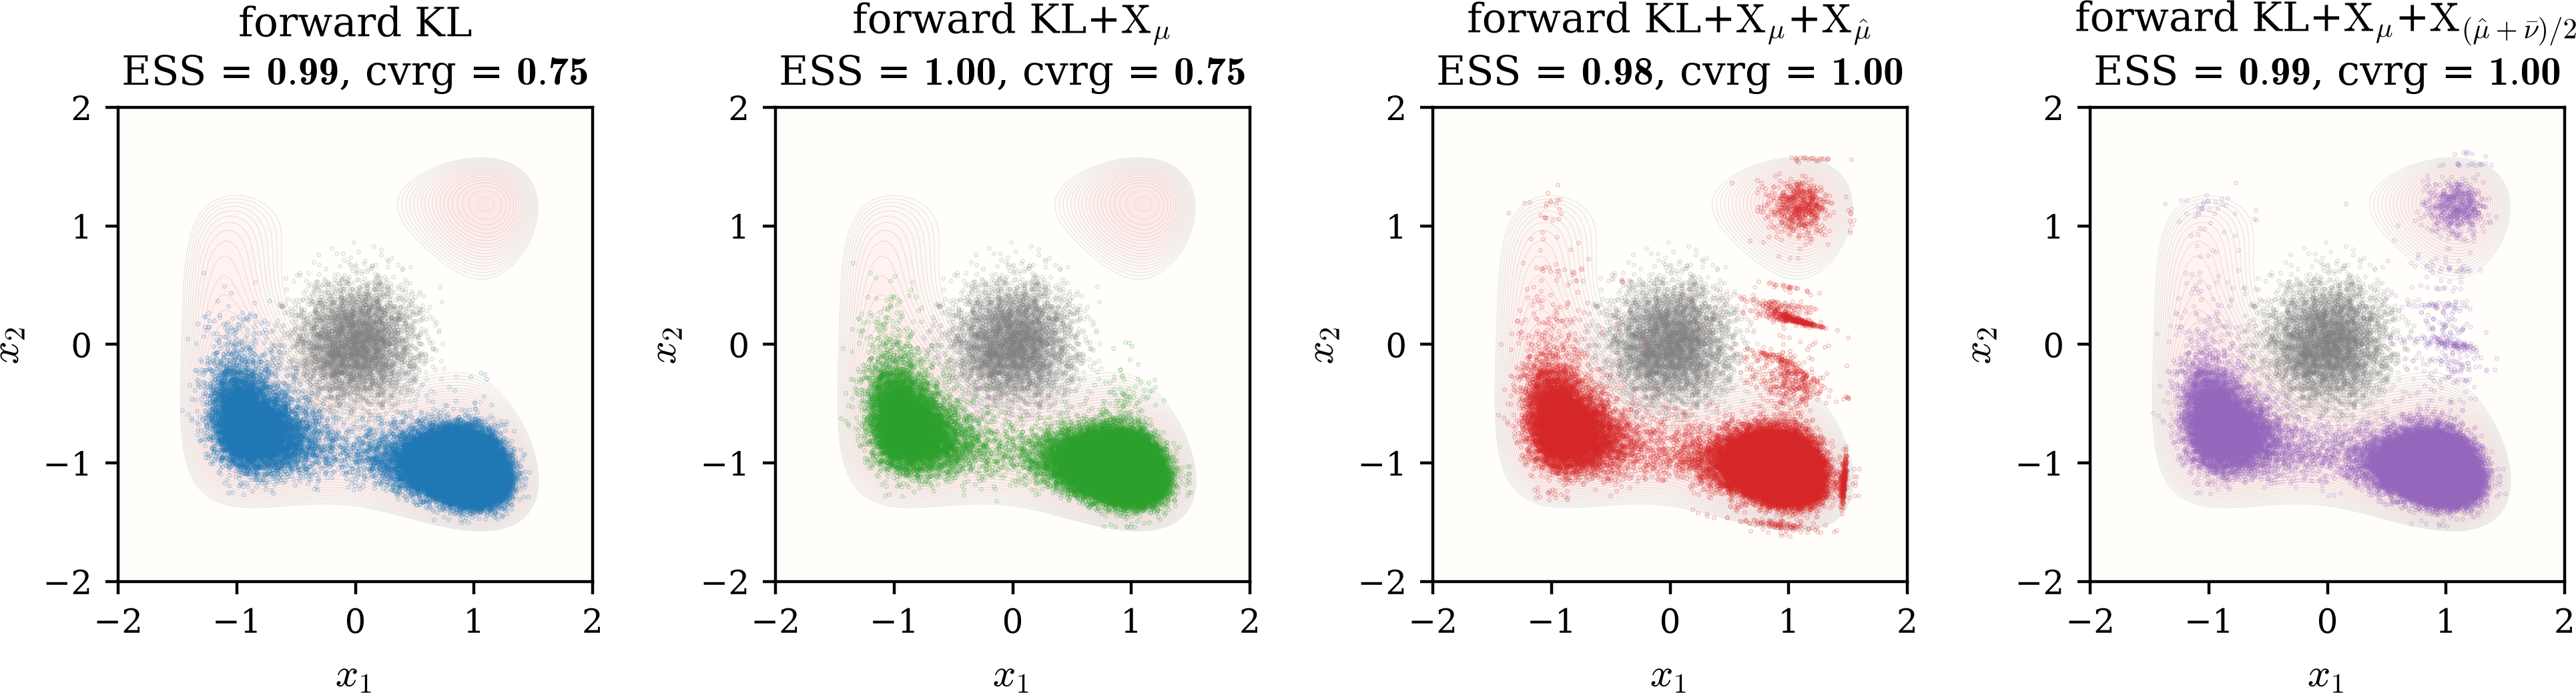
\includegraphics[width=\textwidth]{figures/2D_Benchmark/2D_Threewell/samples.png} \\[0.3em]
        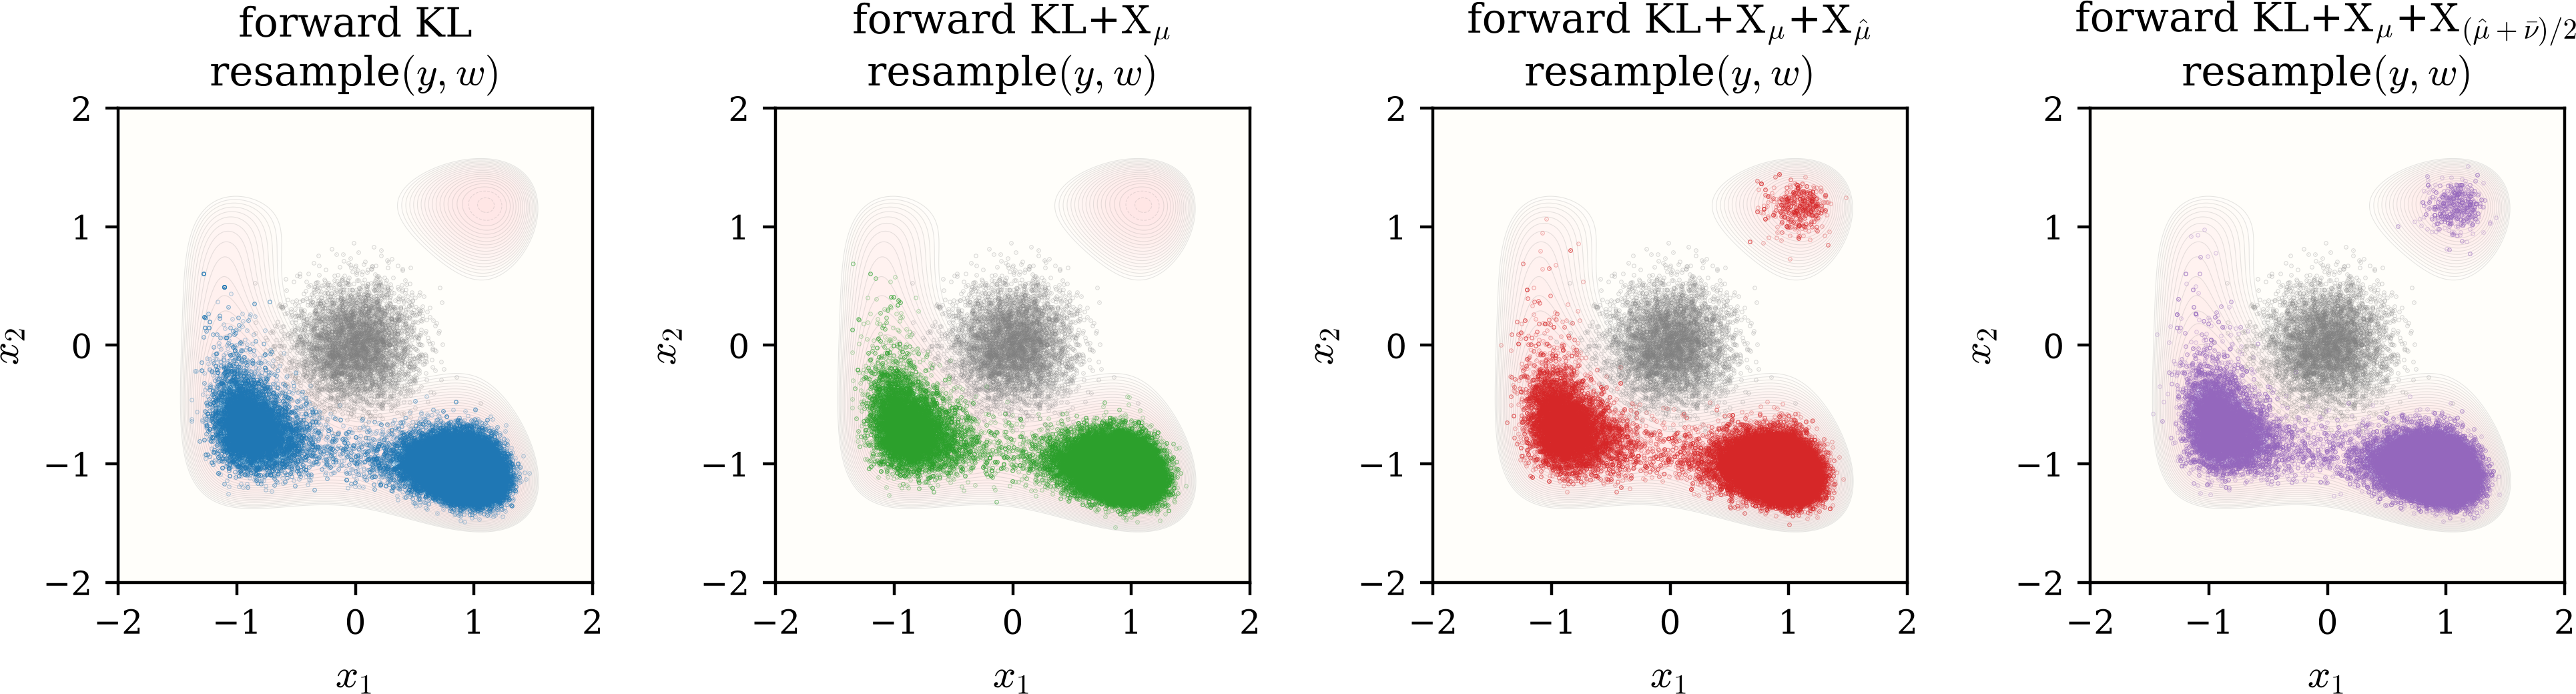
\includegraphics[width=\textwidth]{figures/2D_Benchmark/2D_Threewell/resample.png}
        \caption{Threewell target.}
        \label{fig: threewell}
    \end{subfigure}
    \\[0.8em]
    \begin{subfigure}{\textwidth}
        \centering
        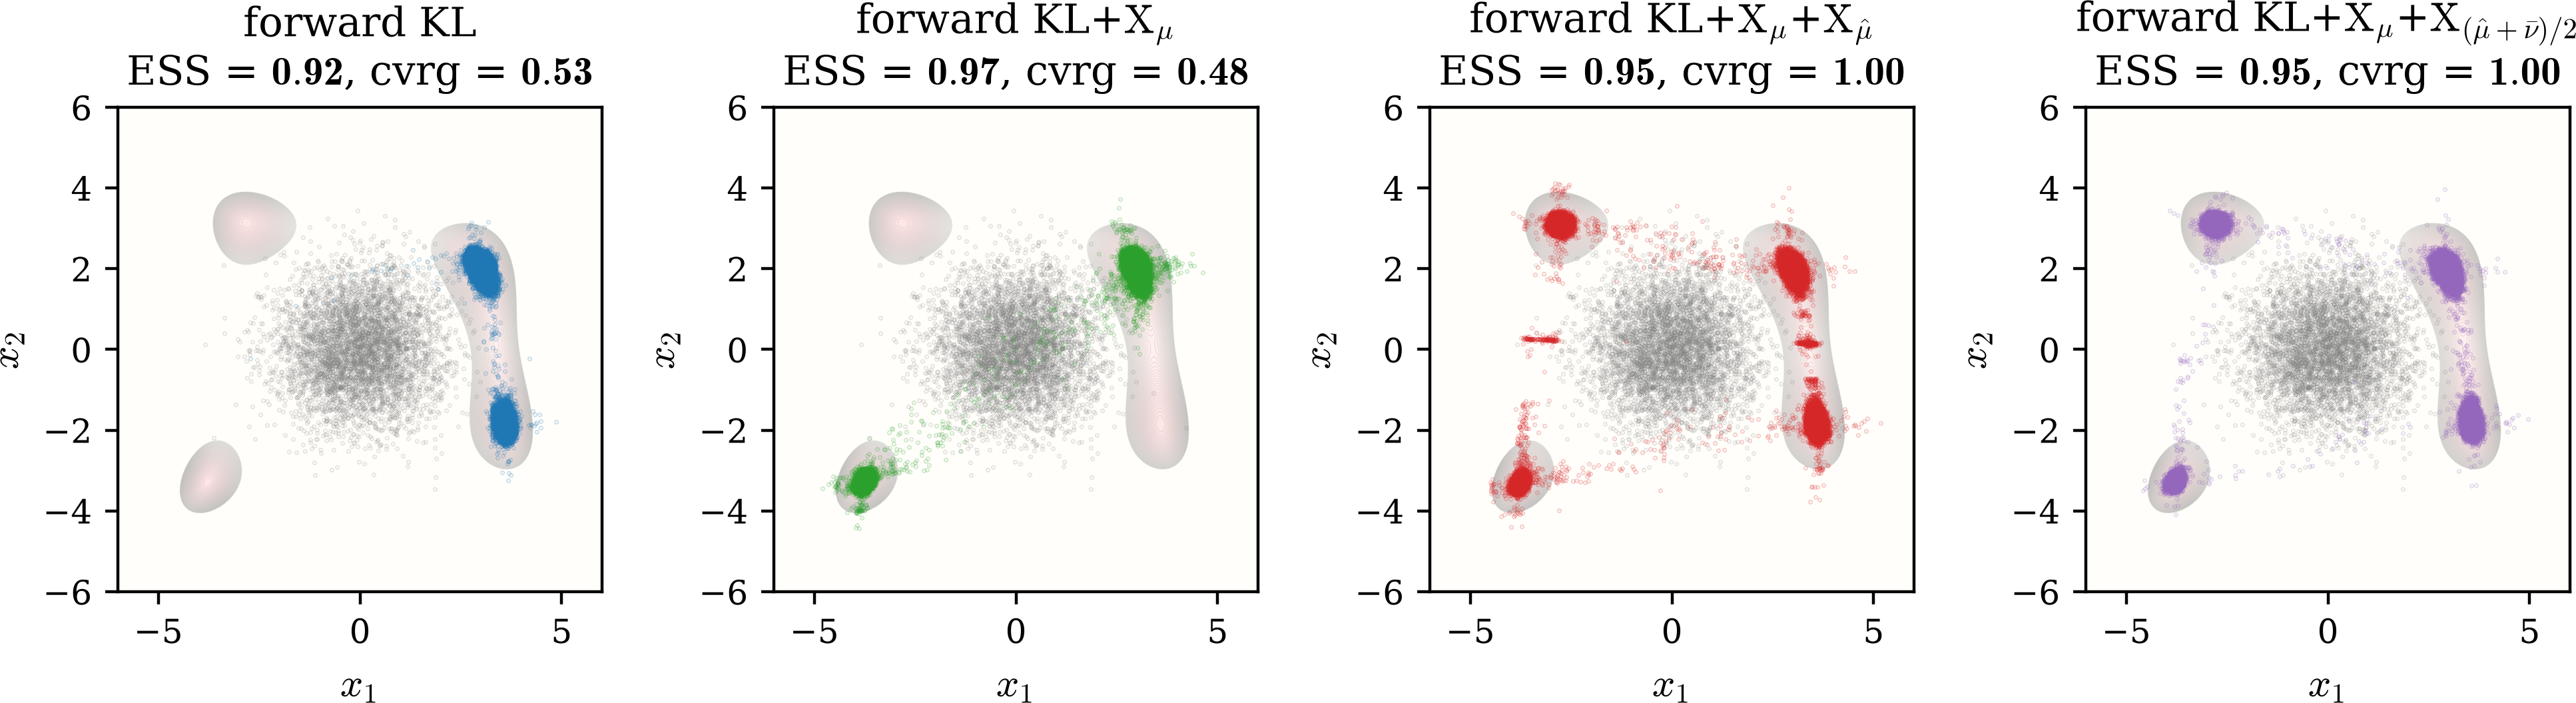
\includegraphics[width=\textwidth]{figures/2D_Benchmark/2D_Himmelblau/samples.png} \\[0.3em]
        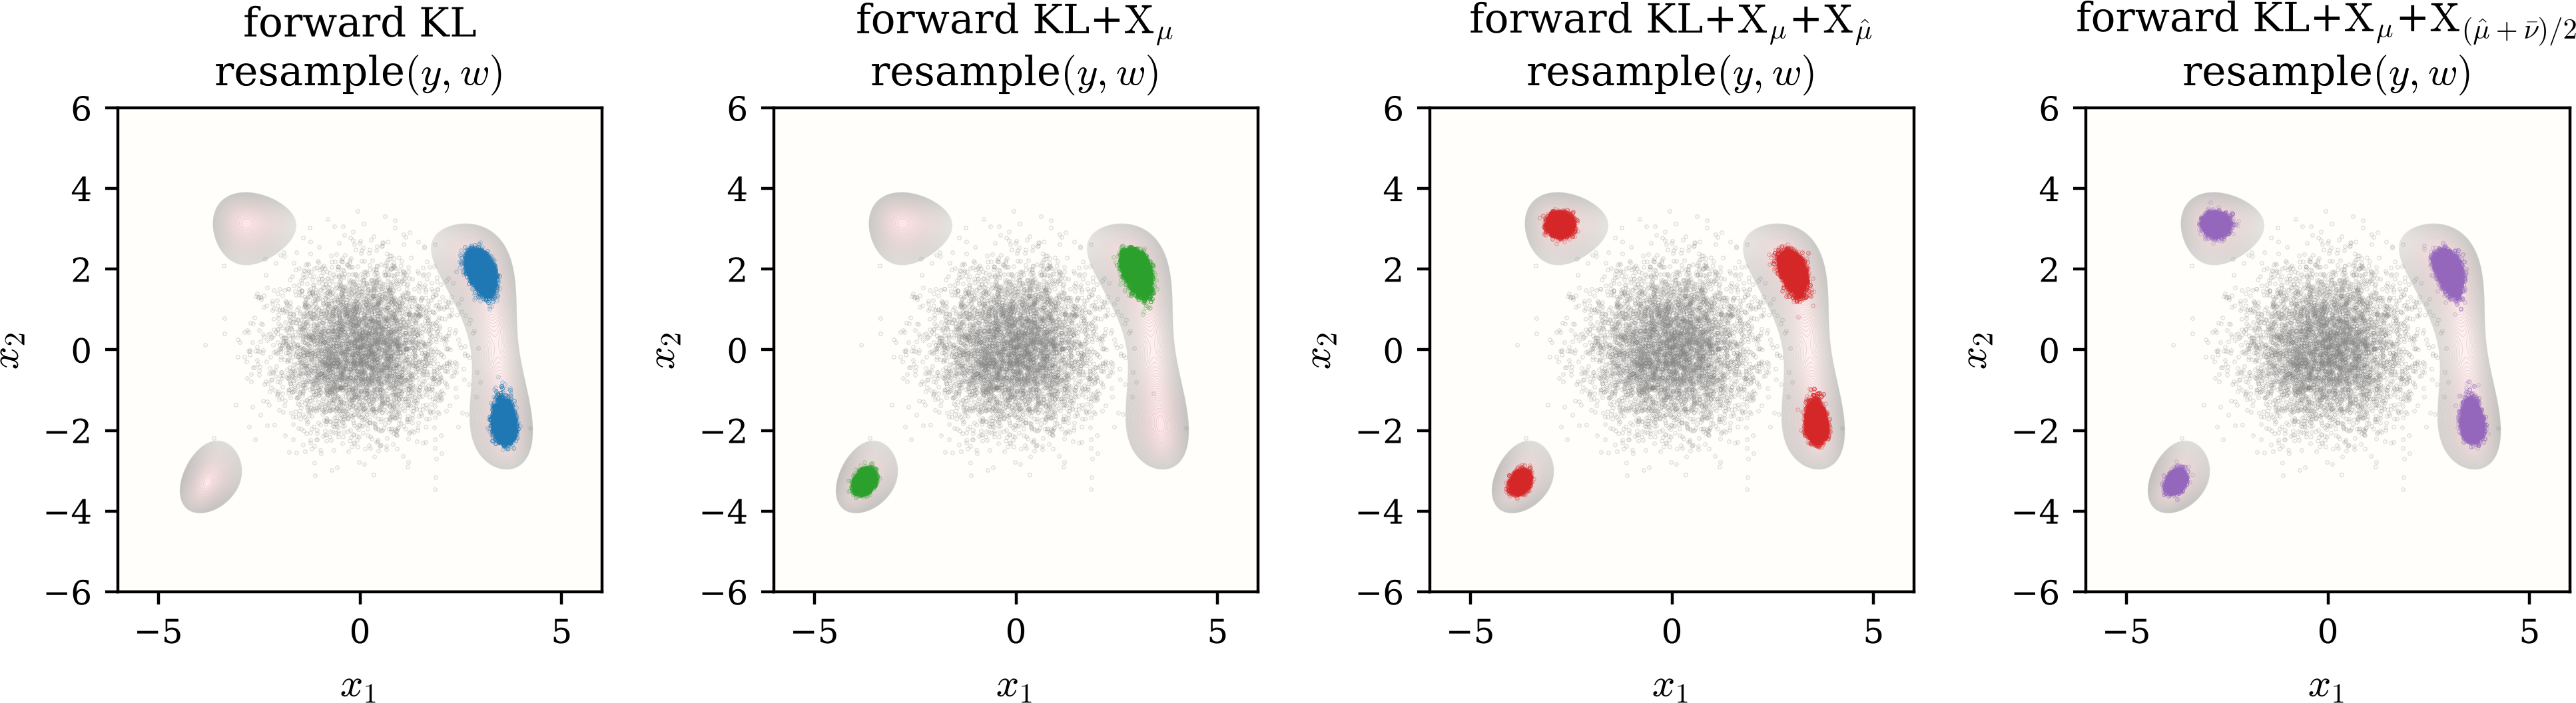
\includegraphics[width=\textwidth]{figures/2D_Benchmark/2D_Himmelblau/resample.png}
        \caption{Himmelblau target.}
        \label{fig: himmelblau}
    \end{subfigure}
    \caption{Mode discovery targets. In each panel, Row 1 is the pushforward $\mathbf{y} = G^{-1}(\mathbf{x})$ and Row 2 is $\mathrm{resample}(\mathbf{y}, w)$ with Langevin rejuvenation. Columns left to right: forward KL, $\KL{+}\X_\mu$, $\KL{+}\X_\mu{+}\X_{\hat\mu}$, $\KL{+}\X_\mu{+}\X_{(\hat\mu+\bar\nu)/2}$. Each pushforward title reports the final ESS and the $\kappa = 5$ coverage against $\hat\mu$.}
    \label{fig: page-mode}
\end{figure}

\paragraph{Annulus.} All four methods reach full coverage, so the discriminator is the flow shape and ESS. Forward KL alone leaves visible axis-aligned filaments across the central barrier; adding $\X_\mu$ tightens the pushforward to a clean ring-plus-point geometry and sharply lifts the ESS, and the mixture ties $\KL{+}\X_\mu$ at the best ESS of the four (Figure~\ref{fig: annulus}). This isolates the role of $\X_\mu$ as a shape regularizer, penalizing pointwise log-ratio variation that the global forward KL leaves untouched.

\paragraph{Python.} The Python target lives on an essentially one-dimensional manifold, the skeleton of the two interlocking snake bodies of the Python logo. All four methods reach full coverage and the ESS plateaus well below $1$. No mode discovery is needed here, yet the X-regularized losses still improve on bare forward KL, and the mixture reaches the best ESS of the four, leading the next-best X variant by $\approx 0.10$ (Figure~\ref{fig: python}) --- consistent with $\bar\nu$ anchoring the off-manifold profile of $\nu$.

\begin{figure}[p]
    \centering
    \begin{subfigure}{\textwidth}
        \centering
        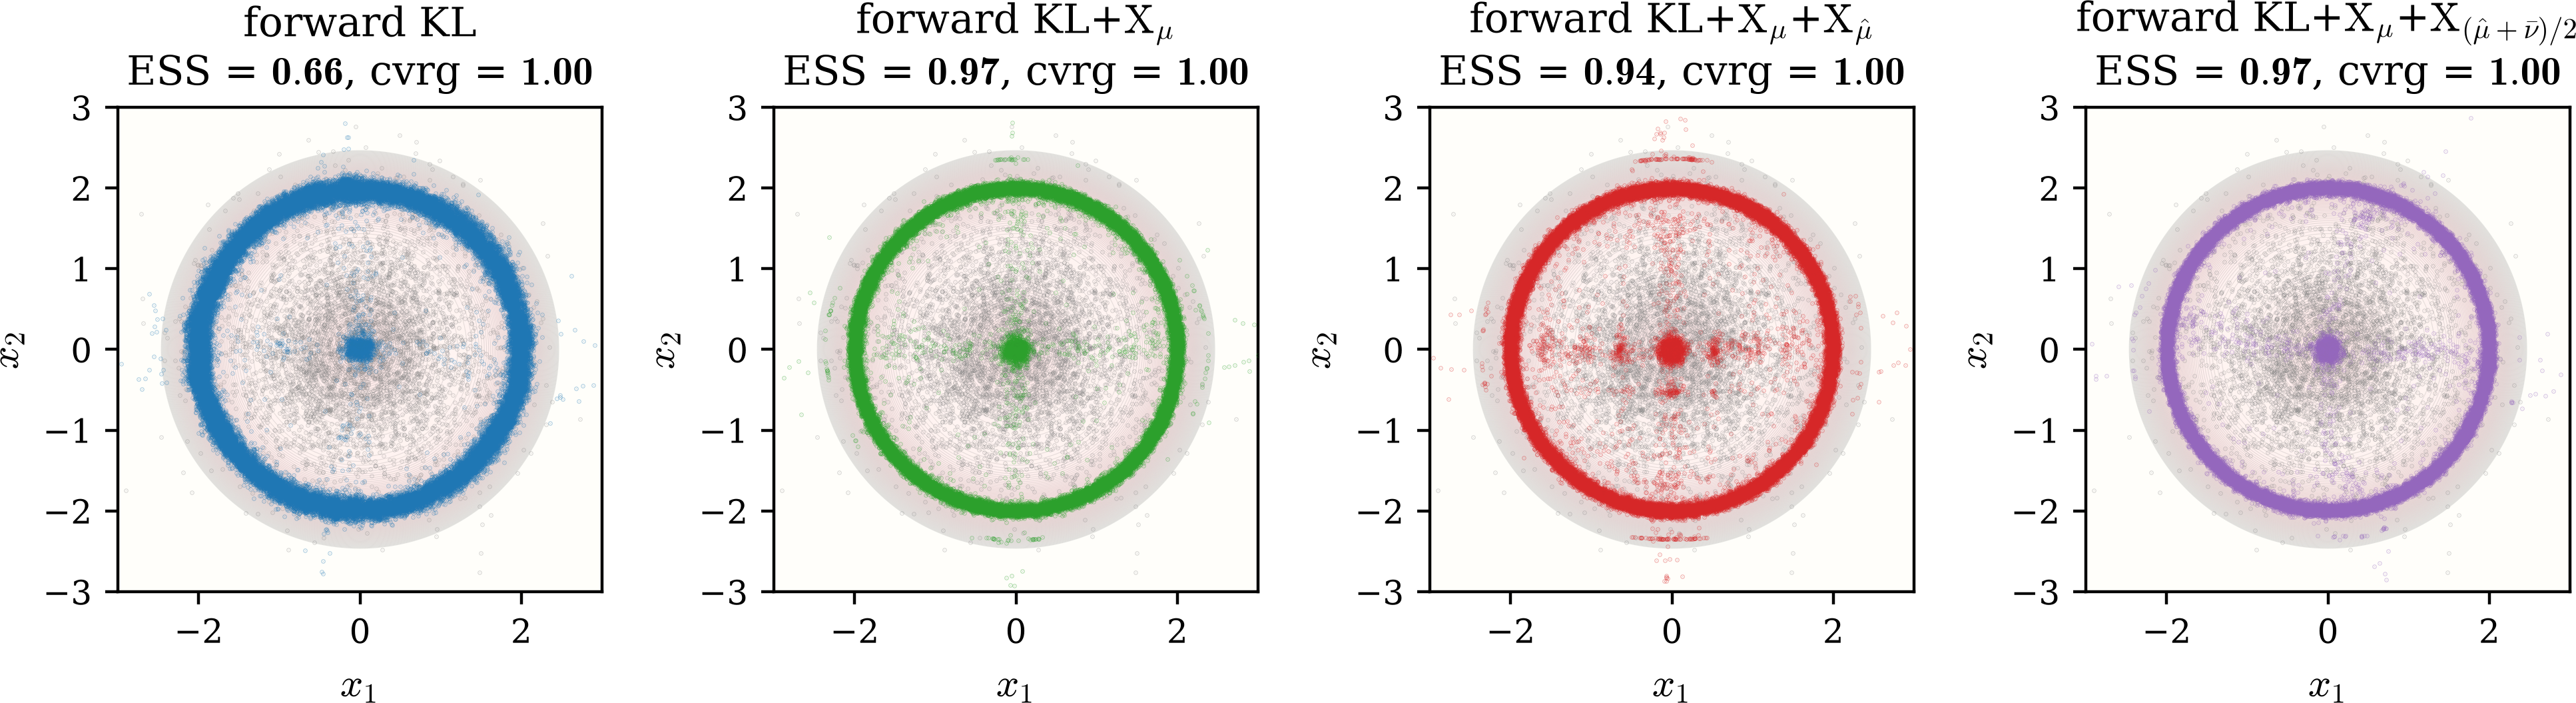
\includegraphics[width=\textwidth]{figures/2D_Benchmark/2D_Annulus/samples.png} \\[0.3em]
        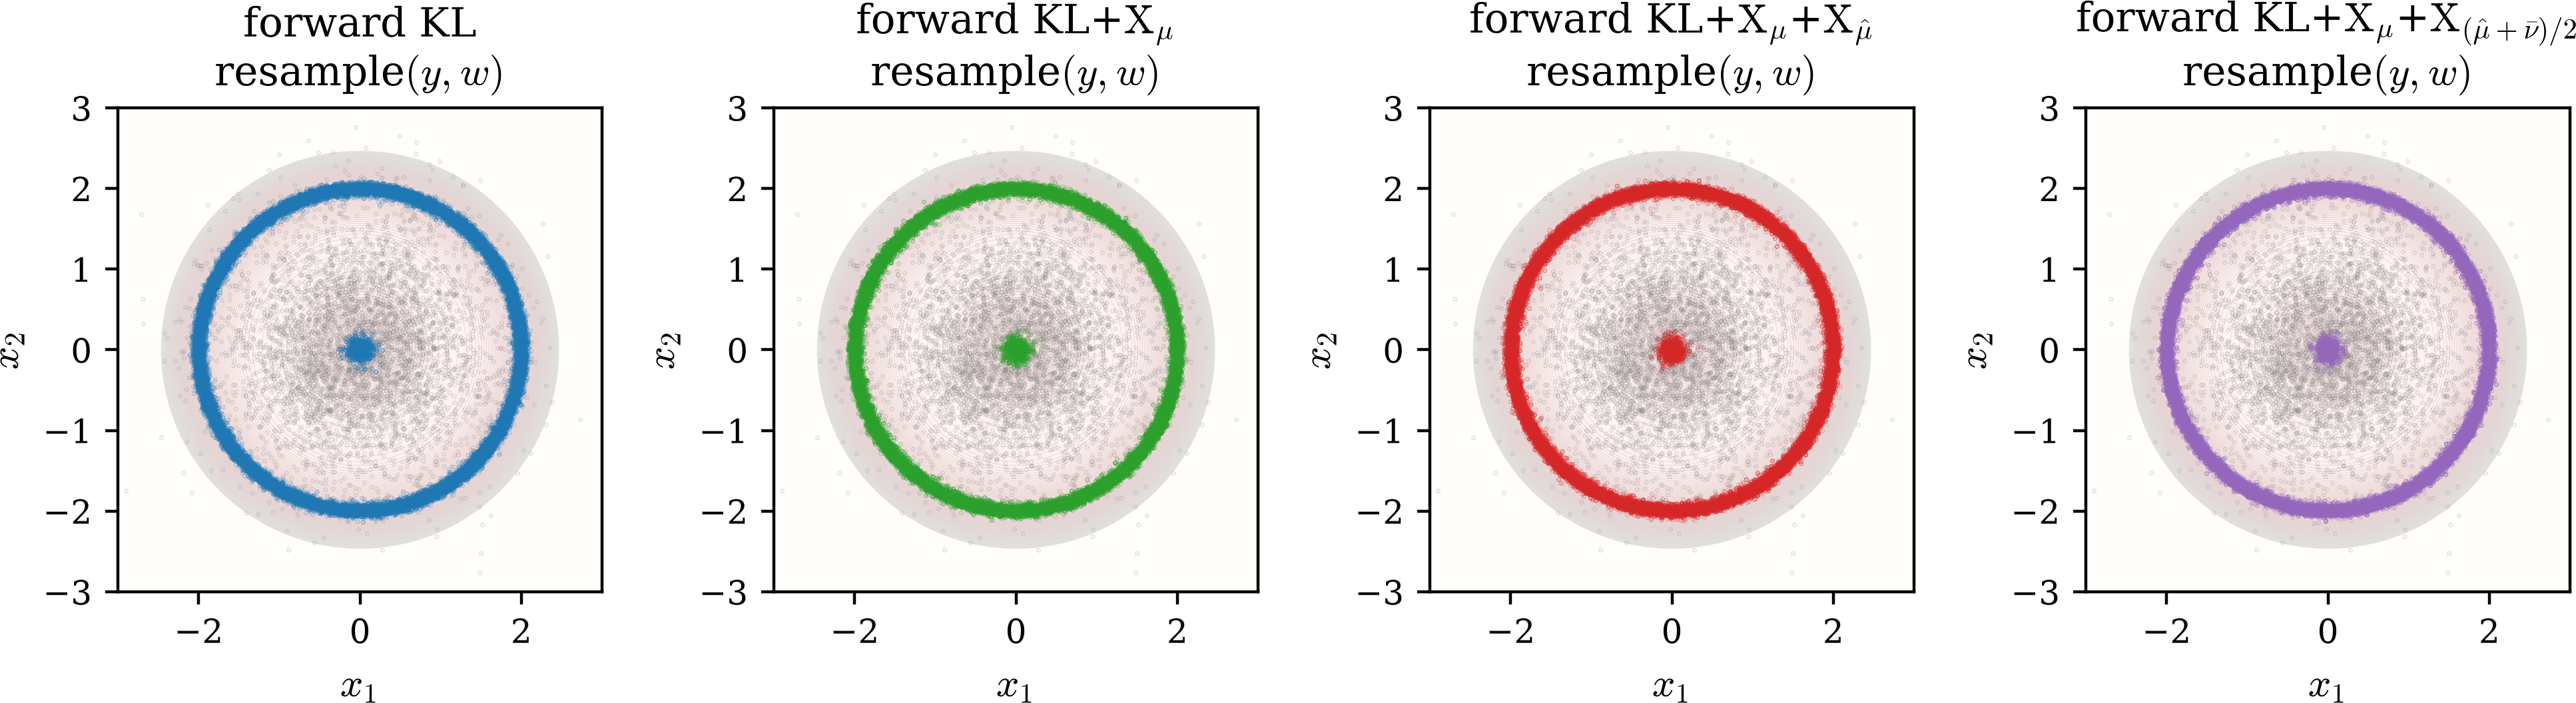
\includegraphics[width=\textwidth]{figures/2D_Benchmark/2D_Annulus/resample.png}
        \caption{Annulus target.}
        \label{fig: annulus}
    \end{subfigure}
    \\[0.8em]
    \begin{subfigure}{\textwidth}
        \centering
        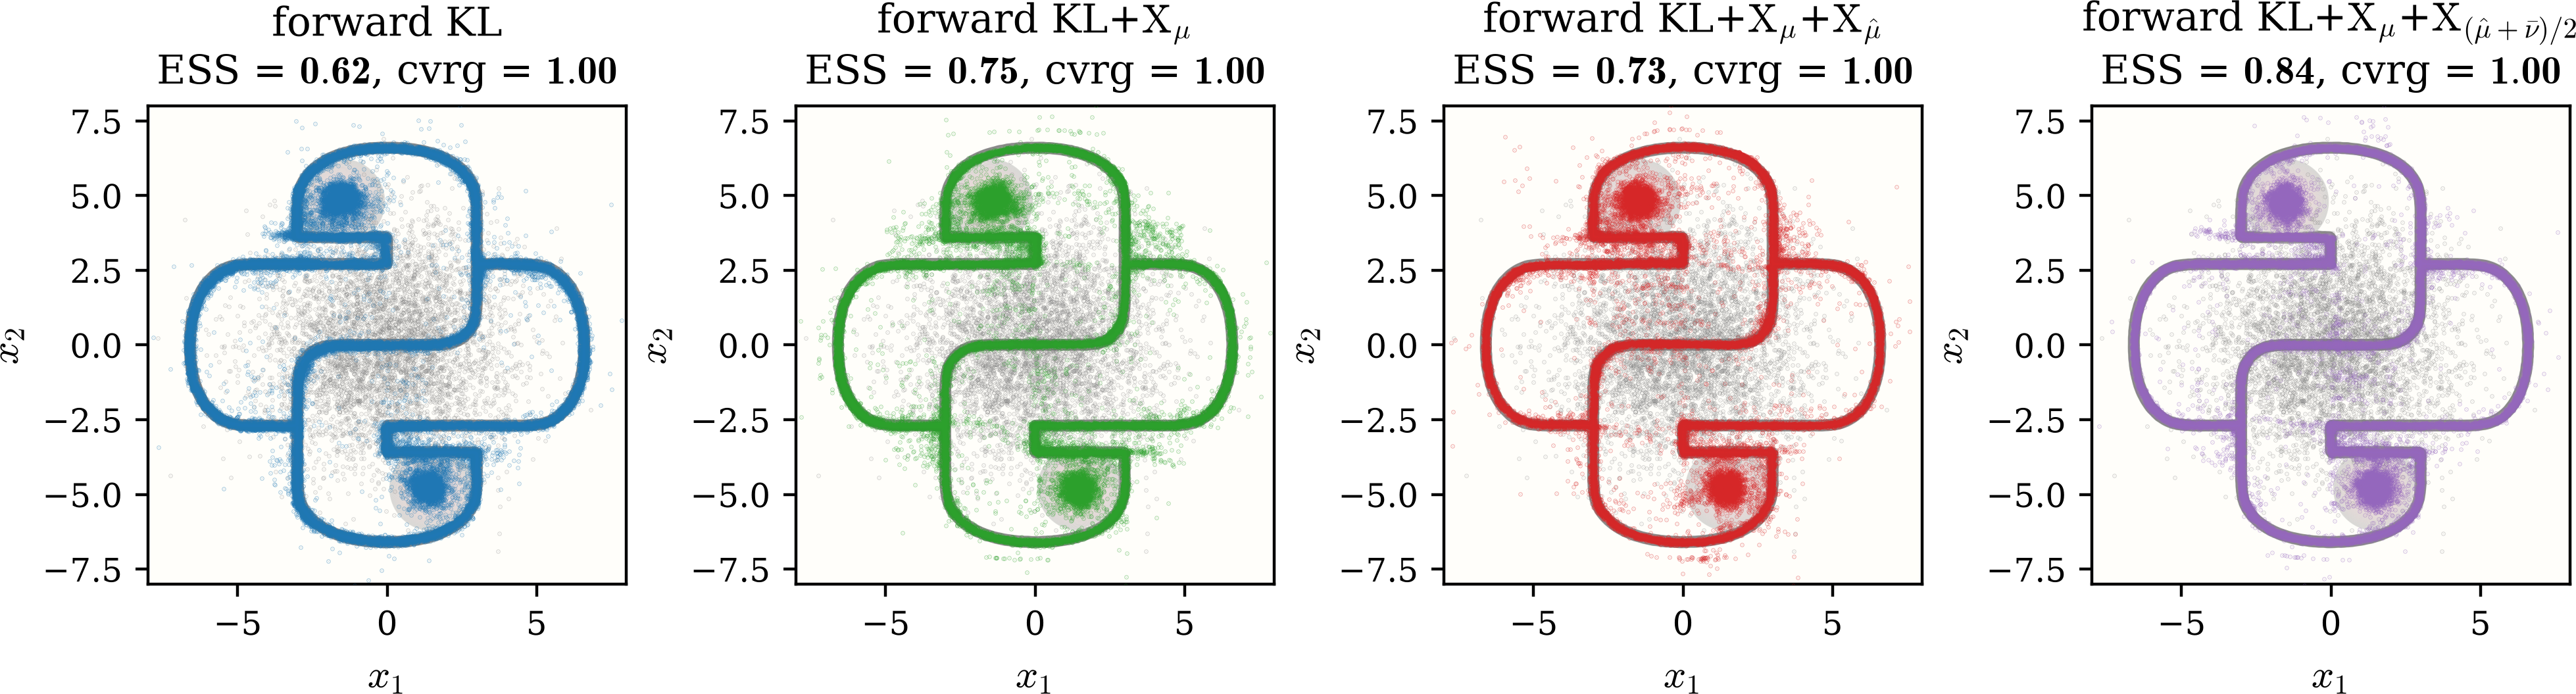
\includegraphics[width=\textwidth]{figures/2D_Benchmark/2D_Python/samples.png} \\[0.3em]
        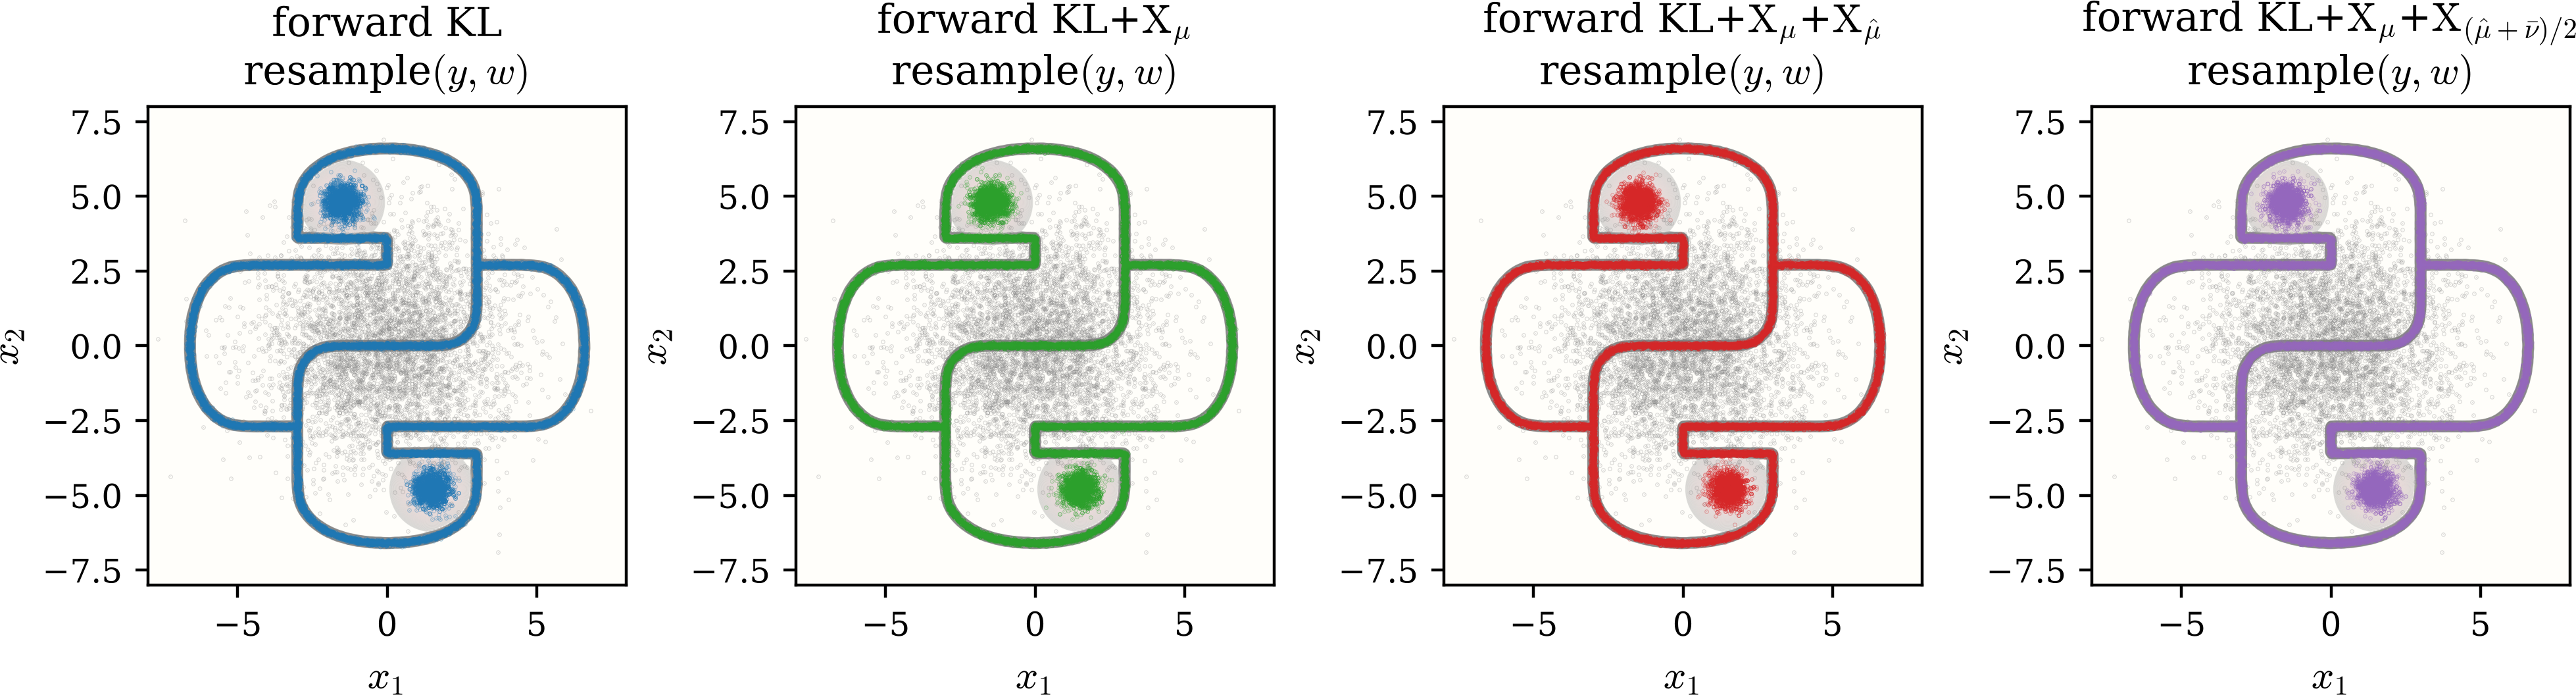
\includegraphics[width=\textwidth]{figures/2D_Benchmark/2D_Python/resample.png}
        \caption{Python target.}
        \label{fig: python}
    \end{subfigure}
    \caption{Shape and manifold targets. Rows and columns as in Figure~\ref{fig: page-mode}.}
\end{figure}

\paragraph{Chessboard.} Coverage is full for all four methods, but mode structure and ESS vary. Forward KL leaks mass into the six removed cells, and neither $\X_\mu$ nor $\X_{\hat\mu}$ stops the leakage: $\hat\mu$ alone is sample-blind to the removed cells. The mixture resolves it: the $\bar\nu$ half sees the holes whenever $\nu$ leaks mass there, and the cross contributions $|\log(\mu/\nu)(\mathbf{y}) - \log(\mu/\nu)(\mathbf{y}')|$ with $\mathbf{y} \sim \hat\mu$ and $\mathbf{y}' \sim \bar\nu$ anchor in-cell and out-of-cell log-ratios to each other, placing mass on the filled cells at the best ESS (Figure~\ref{fig: chessboard}).

\begin{figure}[p]
    \centering
    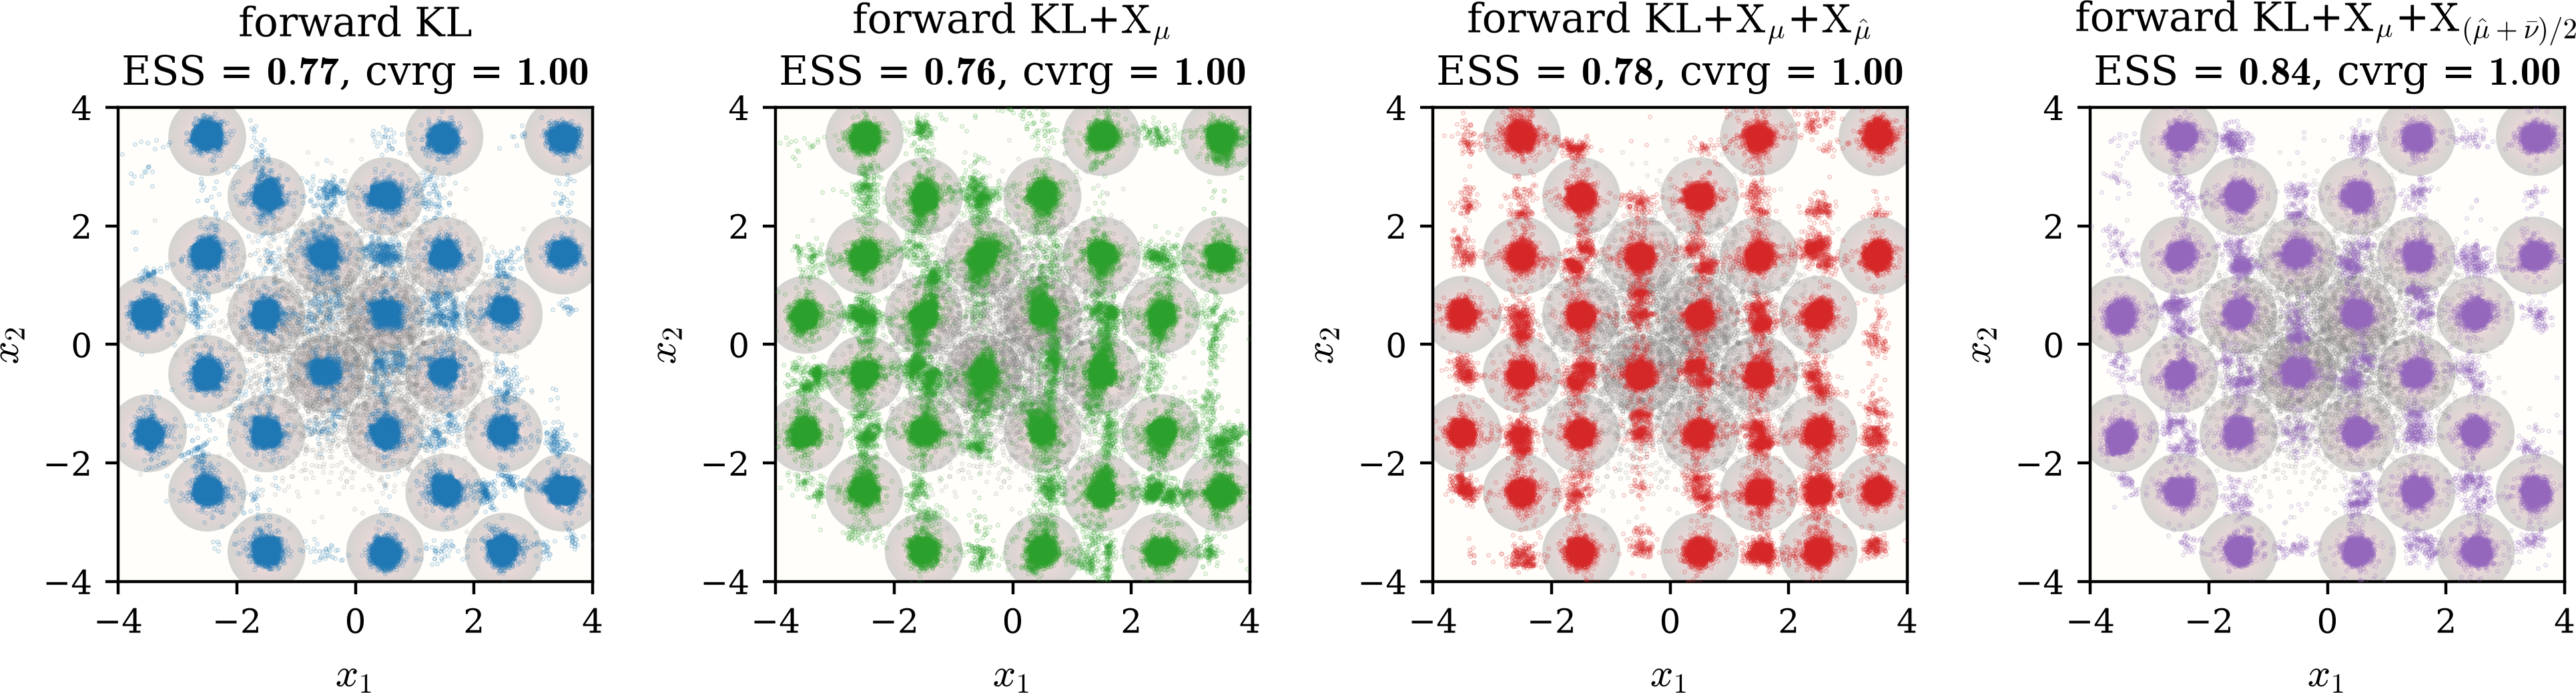
\includegraphics[width=\textwidth]{figures/2D_Benchmark/2D_Chessboard/samples.png} \\[0.6em]
    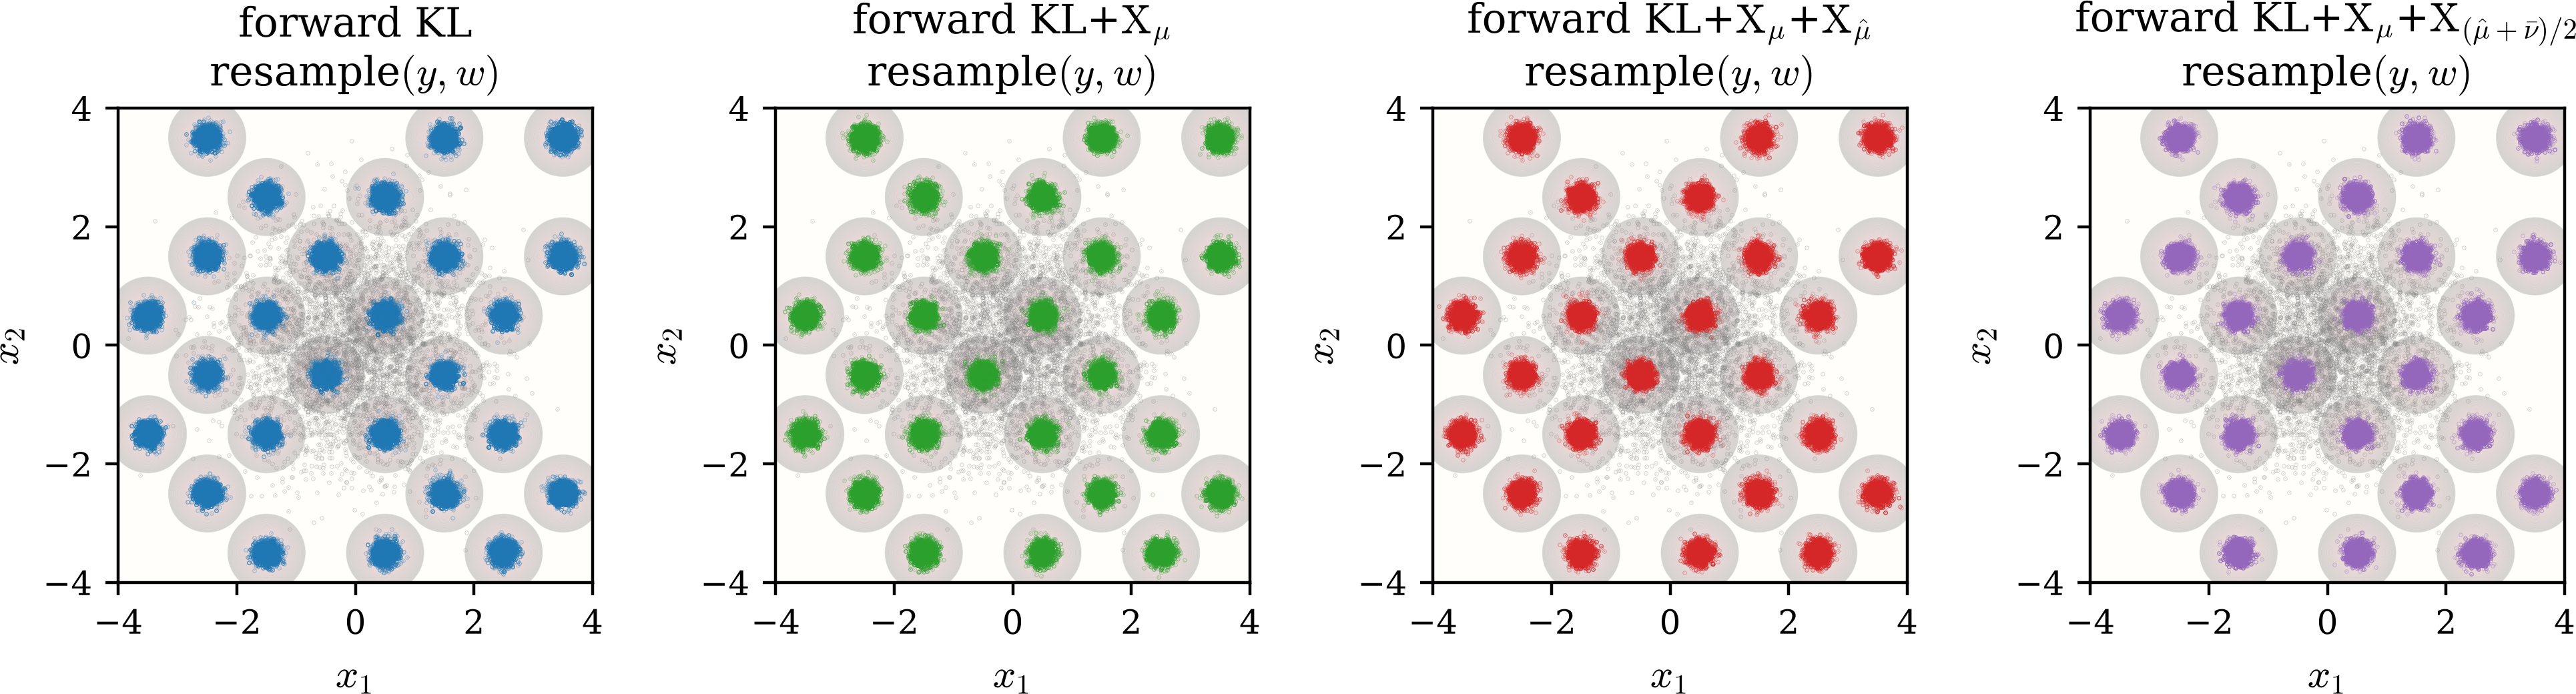
\includegraphics[width=\textwidth]{figures/2D_Benchmark/2D_Chessboard/resample.png}
    \caption{Chessboard target. Row 1: pushforward $\mathbf{y} = G^{-1}(\mathbf{x})$. Row 2: $\mathrm{resample}(\mathbf{y}, w)$ with Langevin rejuvenation. Columns as in Figure~\ref{fig: page-mode}.}
    \label{fig: chessboard}
\end{figure}

\paragraph{Sparse.} A four-mode Gaussian mixture with a dense central pair and two isolated corner modes the narrow source cannot reach. Forward KL and $\KL{+}\X_\mu$ lock onto the central pair and miss the corners at high, stable ESS, another fake ESS instance. Adding $\X_{\hat\mu}$ restores full coverage but, lacking the $\bar\nu$ half, overfits $\hat\mu$ and leaves artificial bridges of mass between the modes; the mixture also reaches full coverage while removing these bridges, at the best full-coverage ESS (Figure~\ref{fig: sparse}).

\begin{figure}[p]
    \centering
    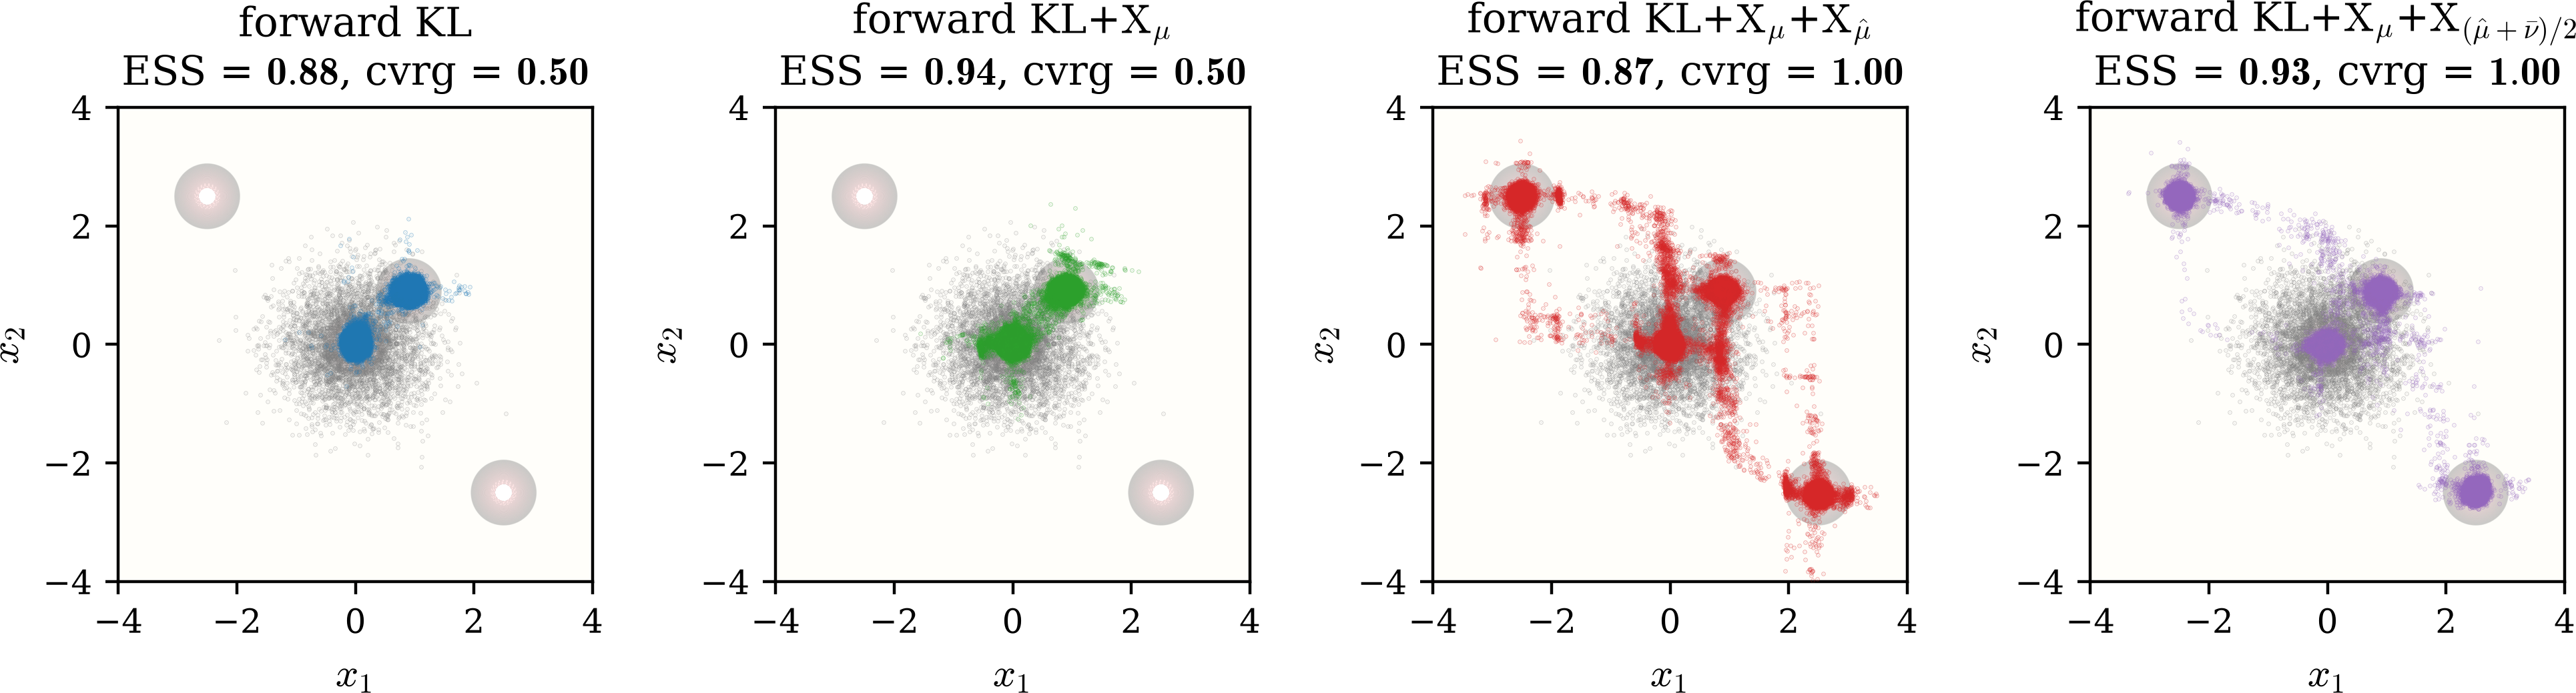
\includegraphics[width=\textwidth]{figures/2D_Benchmark/2D_Sparse/samples.png} \\[0.6em]
    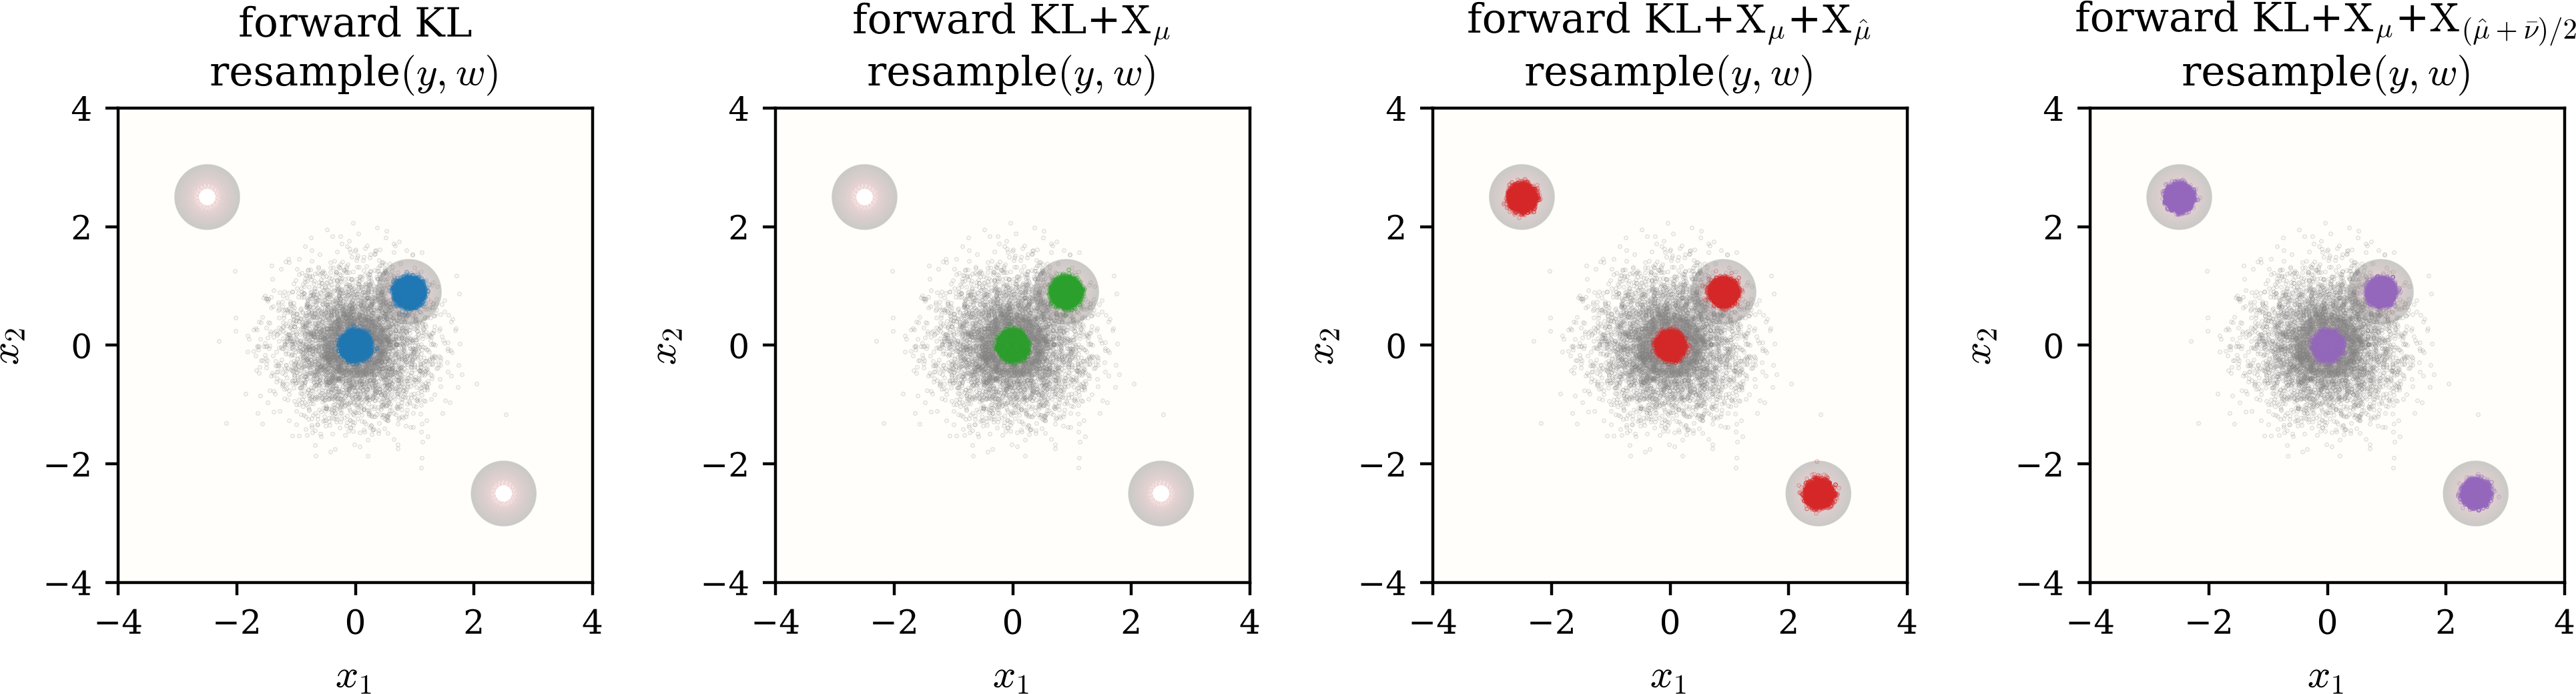
\includegraphics[width=\textwidth]{figures/2D_Benchmark/2D_Sparse/resample.png}
    \caption{Sparse target. Row 1: pushforward $\mathbf{y} = G^{-1}(\mathbf{x})$. Row 2: $\mathrm{resample}(\mathbf{y}, w)$ with Langevin rejuvenation. Columns as in Figure~\ref{fig: page-mode}.}
    \label{fig: sparse}
\end{figure}

\begin{table}[h]
    \centering
    \begin{tabular}{@{}lcccc@{}}
        \toprule
        target & KL & $\KL{+}\X_\mu$ & $\KL{+}\X_\mu{+}\X_{\hat\mu}$ & $\KL{+}\X_\mu{+}\X_{(\hat\mu+\bar\nu)/2}$ \\
        \midrule
        Threewell  & $0.99\,(0.75)$ & $1.00\,(0.75)$ & $0.98\,(1.00)$ & $\mathbf{0.99}\,(1.00)$ \\
        Himmelblau & $0.92\,(0.53)$ & $0.97\,(0.48)$ & $\mathbf{0.95}\,(1.00)$ & $\mathbf{0.95}\,(1.00)$ \\
        Annulus    & $0.66\,(1.00)$ & $\mathbf{0.97}\,(1.00)$ & $0.94\,(1.00)$ & $\mathbf{0.97}\,(1.00)$ \\
        Python     & $0.62\,(1.00)$ & $0.75\,(1.00)$ & $0.73\,(1.00)$ & $\mathbf{0.84}\,(1.00)$ \\
        Chessboard & $0.77\,(1.00)$ & $0.76\,(1.00)$ & $0.78\,(1.00)$ & $\mathbf{0.84}\,(1.00)$ \\
        Sparse     & $0.88\,(0.50)$ & $0.94\,(0.50)$ & $0.87\,(1.00)$ & $\mathbf{0.93}\,(1.00)$ \\
        \bottomrule
    \end{tabular}
    \caption{Final ESS, with $\kappa=5$ coverage against $\hat\mu$ in parentheses, for each loss on each 2D target; the best full-coverage ESS per row is in bold.}
    \label{tab: 2d-benchmark-summary}
\end{table}

Across the six targets two regimes emerge (Table~\ref{tab: 2d-benchmark-summary}). On the mode discovery targets Threewell, Himmelblau, and Sparse, the ESS stays high for every loss and is therefore useless on its own: forward KL and $\KL{+}\X_\mu$ post ESS up to $1.00$ while silently missing modes, and only the $\X_{\hat\mu}$ and mixture variants restore full coverage. On the shape, manifold, and leakage targets Annulus, Python, and Chessboard, coverage is already complete and ESS becomes the discriminator: $\X_\mu$ helps on Annulus and Python but is flat on Chessboard, whereas the mixture improves on bare forward KL by $+0.31$, $+0.22$, and $+0.07$ and attains the best ESS on all three. Overall the mixture is the only loss of the four that reaches full mode coverage and the best or tied-best full-coverage ESS on every target, and its ESS curves are smoother than bare forward KL.

The mixture loss $\mathcal L = \KL(\mu \| \nu) + \X_\mu(\mu\|\nu) + \X_{(\hat\mu + \bar\nu)/2}(\mu\|\nu)$ with $\lambda = 1$ and $\alpha = \beta = \frac12$ is the recommended default. It absorbs the mode discovery role of $\X_{\hat\mu}$ while suppressing the leakage that $\X_{\hat\mu}$ alone can introduce when the target has holes interleaved with its modes.

\subsection{Bayesian inverse problem: sensor-array source localization}
\label{subsec: sensor}

Our next benchmark is a physical Bayesian inverse problem where the multimodality comes from a symmetry of the measurement, not from a hand-built mixture. The setting is source localization, a standard problem in acoustics and signal processing: a line of fixed sensors records the combined signal of several identical point sources, and we infer the source positions from the noisy readings. The unknown is the vector of source positions $\boldsymbol{\theta} = (\theta_1, \dots, \theta_n) \in \mathbb R^n$ for $n = 3$ sources. A source at $\theta_i$ leaves a Gaussian bump of width $\ell = 0.8$ at each sensor and the sensors read the sum, so with $J = 25$ sensors at fixed positions $s_1, \dots, s_J$ equispaced on $[-6, 6]$ the reading at sensor $j$ is
\begin{equation*}
    g_j(\boldsymbol{\theta}) \;=\; \sum_{i=1}^{n} \exp\!\Bigl( -\frac{(s_j - \theta_i)^2}{2\ell^2} \Bigr).
\end{equation*}
The data are these readings at the true positions $\boldsymbol{\theta}^\star = (5, 0, -5)$ with i.i.d.\ Gaussian noise,
\begin{equation*}
    y_j \;=\; g_j(\boldsymbol{\theta}^\star) + \varepsilon_j, \qquad \varepsilon_j \sim \mathcal N(0, \sigma_{\mathrm{obs}}^2), \quad \sigma_{\mathrm{obs}} = 0.3,
\end{equation*}
fixed across all losses. The prior on the positions is a centered isotropic Gaussian $\mu_0 = \mathcal N(0, \sigma_{\mathrm{prior}}^2 I_n)$ with $\sigma_{\mathrm{prior}} = 1.6$, which is also the flow's source, and the negative log-posterior is the prior plus the data fit,
\begin{equation}
    U(\boldsymbol{\theta}) \;=\; \frac{1}{2\sigma_{\mathrm{obs}}^2} \sum_{j=1}^{J} \bigl( g_j(\boldsymbol{\theta}) - y_j \bigr)^2 \;+\; \frac{1}{2\sigma_{\mathrm{prior}}^2}\,\|\boldsymbol{\theta}\|^2 .
    \label{eq: sensor-potential}
\end{equation}

Because the sources are identical, $g_j$ is a sum over them and is unchanged by any permutation of the coordinates, $g_j(\theta_{\pi(1)}, \dots, \theta_{\pi(n)}) = g_j(\boldsymbol{\theta})$ for $\pi \in S_3$; the prior is permutation-invariant too, so $U(\pi\cdot\boldsymbol{\theta}) = U(\boldsymbol{\theta})$. The posterior therefore has $3! = 6$ equal, well-separated modes, the permutations of $\boldsymbol{\theta}^\star$, and the centered prior sits on their common symmetry point at the origin, about $4.4$ prior standard deviations from every mode, $\|\boldsymbol{\theta}^\star\| = 7.07$. The prior tail reaches none of them, so a flow trained by bare forward KL only sees the one or two modes its pushforward first lands on and collapses there. We use the same flow, training, and diagnostics as Section~\ref{subsec: 2d-benchmark}.

Table~\ref{tab: sensor-result} and Figure~\ref{fig: sensor} report the comparison. Bare forward KL covers only $2$ of the $6$ modes at ESS $0.90$, and adding $\X_\mu$ posts the highest ESS of the four, $0.98$, while collapsing onto a single mode --- the ESS improves as coverage gets worse. The QT-driven $\X_{\hat\mu}$ and the mixture both recover all $6$ modes, with mass split evenly, at ESS $0.91$ and $0.93$.

\begin{table}[h]
    \centering
    \begin{tabular}{@{}lcc@{}}
        \toprule
        loss & final ESS & modes found \\
        \midrule
        forward KL                                & 0.904 & 2 \\
        $\KL{+}\X_\mu$                             & $\mathbf{0.979}$ & 1 \\
        $\KL{+}\X_\mu{+}\X_{\hat\mu}$              & 0.913 & $\mathbf{6}$ \\
        $\KL{+}\X_\mu{+}\X_{(\hat\mu+\bar\nu)/2}$  & 0.934 & $\mathbf{6}$ \\
        \bottomrule
    \end{tabular}
    \caption{Sensor-array source-localization benchmark \eqref{eq: sensor-potential} with $n = 3$ sources and $3! = 6$ permutation modes.}
    \label{tab: sensor-result}
\end{table}

\begin{figure}[h]
    \centering
    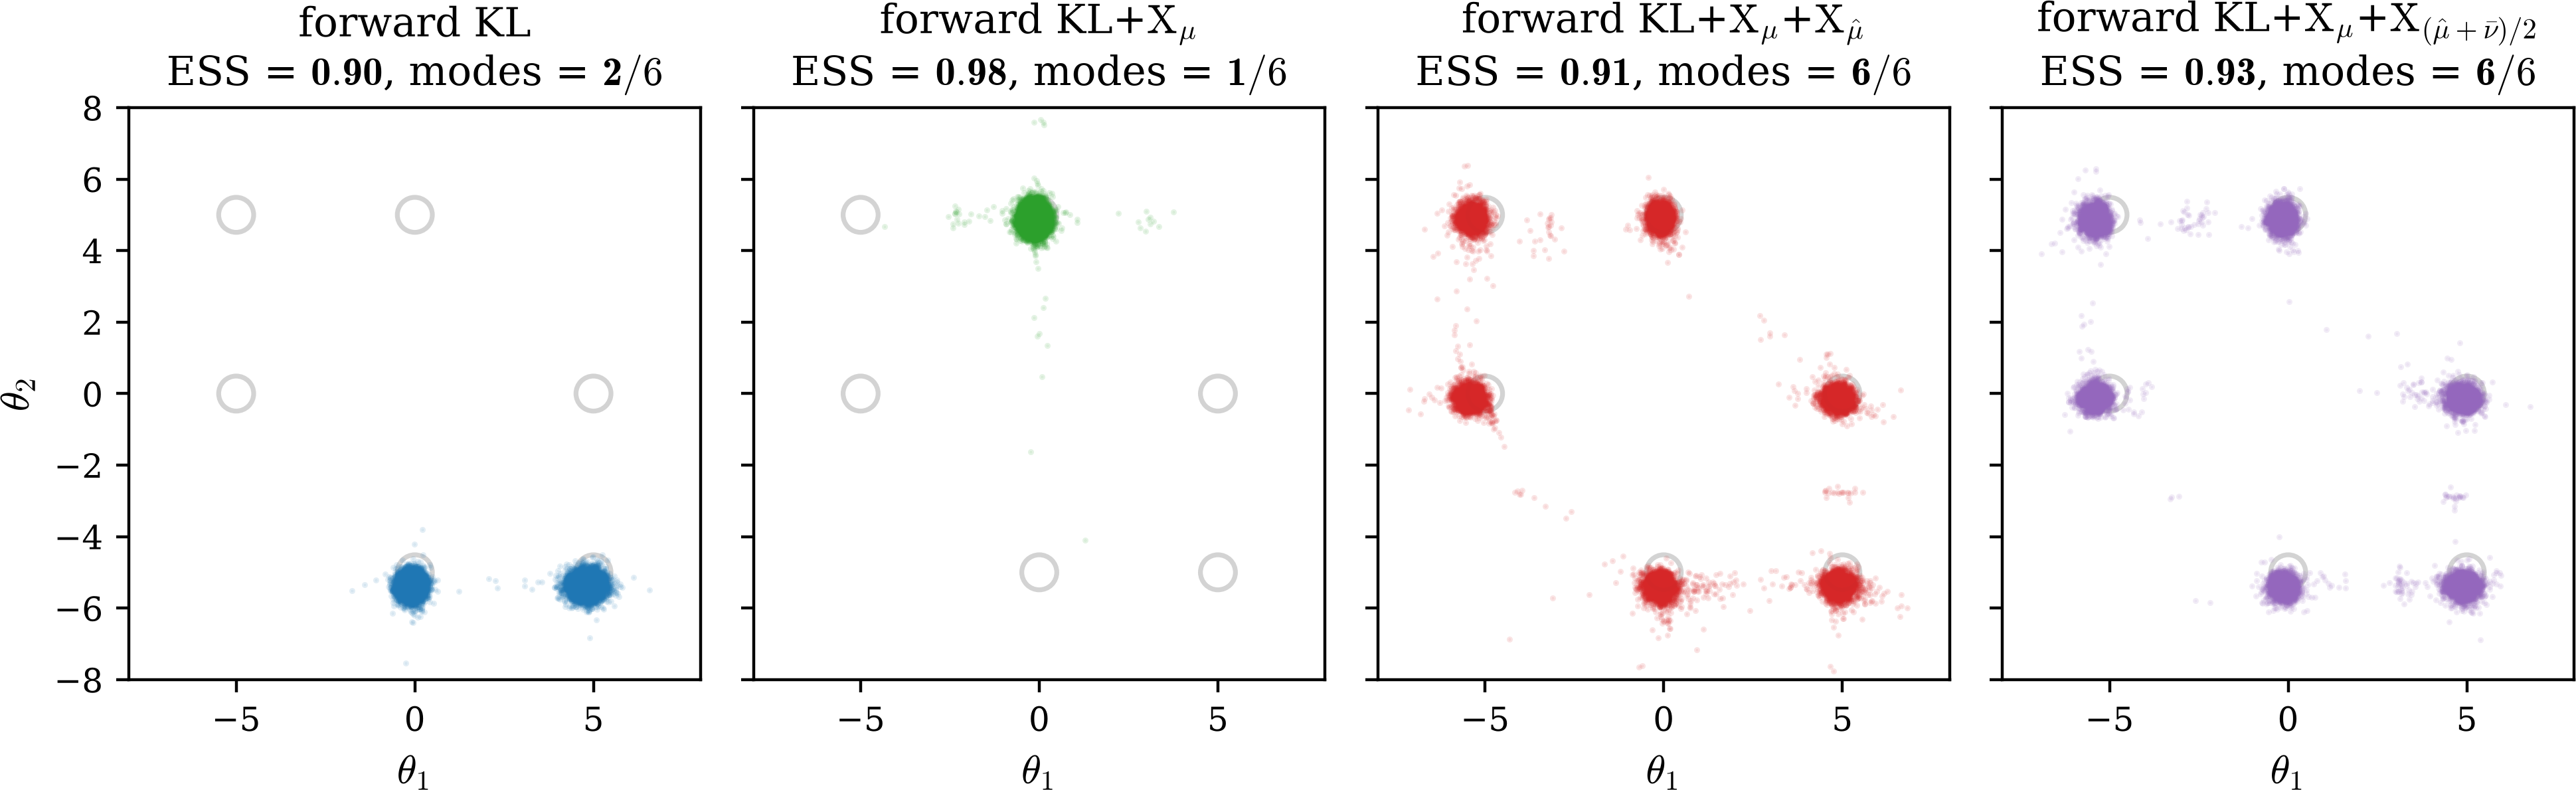
\includegraphics[width=\textwidth]{figures/Sensor_Array/samples.png} \\[0.4em]
    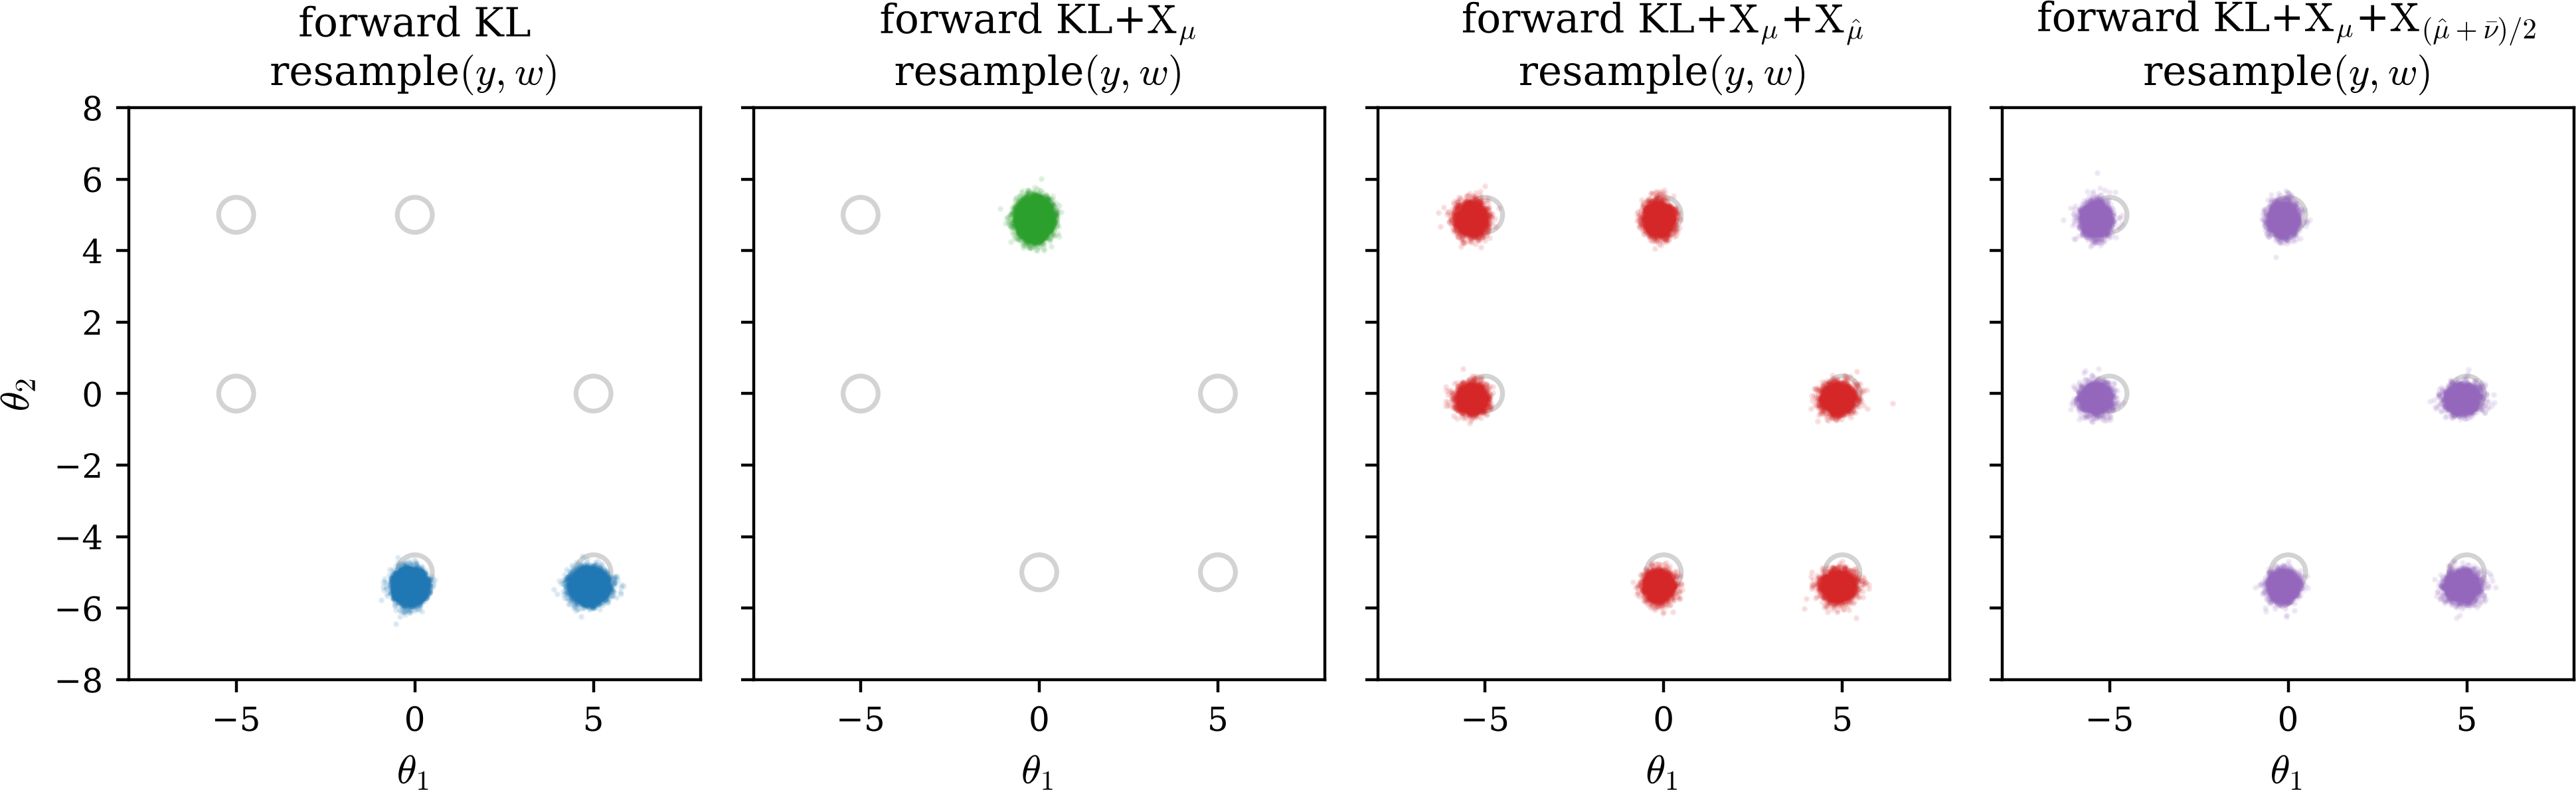
\includegraphics[width=\textwidth]{figures/Sensor_Array/resample.png}
    \caption{Sensor-array posterior, pushforward positions projected onto $(\theta_1, \theta_2)$. Row 1: raw pushforward $\mathbf{y} = G^{-1}(\mathbf{x})$; Row 2: $\mathrm{resample}(\mathbf{y}, w)$ with Langevin rejuvenation. Columns left to right: forward KL, $\KL{+}\X_\mu$, $\KL{+}\X_\mu{+}\X_{\hat\mu}$, $\KL{+}\X_\mu{+}\X_{(\hat\mu+\bar\nu)/2}$. Light-gray circles mark the six permutation mode centers; each title reports the final ESS and the modes found out of six.}
    \label{fig: sensor}
\end{figure}

This benchmark is intentionally low-dimensional, and the numbers come from a single training seed; which modes a collapsed method happens to keep is set by the random path, not by the loss.

\subsection{High-dimensional product multi-well}
\label{subsec: highd}

To test the framework beyond two dimensions we construct a family of product multi-well targets in dimension $d = 2^k$, playing here the role that double-well systems play in the diffusion-sampler literature \citep{akhound2024iterated,woo2024iefm}, but with an analytically known mode structure and a diagonal optimal transport map so that training failures are unambiguously training failures and not capacity failures of the flow,
\begin{equation}
    U(\mathbf{x}) = \frac12 \sum_{i=1}^{2^k} x_i^2 + 12 \sum_{i=1}^{k} \exp(-x_i^2),
    \label{eq: highd-potential}
\end{equation}
a double well in each of the first $k$ coordinates, with minima at $\pm\sqrt{\ln 24} \approx \pm 1.78$ separated by a barrier of height $\approx 9.9$, and a standard Gaussian in the remaining $2^k - k$. The source is the standard Gaussian $\mu_0 = \mathcal N(0, I_d)$, whose potential is the quadratic part of $U$. Because $U$ is separable, the target factorizes into $k$ identical double wells and $2^k - k$ Gaussians, so it has exactly $2^k = d$ modes, and the optimal transport map is diagonal. The source sits exactly on the barrier of every double well, so the untrained pushforward covers none of the $2^k$ mode combinations. We sweep $k = 1, \dots, 8$, i.e.\ $d = 2, 4, 8, 16, 32, 64, 128, 256$.

The flow is a neural spline flow on $[-4, 4]^d$ with $6$ coupling transforms, $16$ bins, and hidden widths $(256, 256)$. Training uses Adam at learning rate $10^{-3}$ with batch size $200$, drawn from a source set of $10^4 \cdot 2^k$ samples; forward KL is sensitive to the batch size, so the small batch sharpens the contrast between the losses. The number of steps decreases with $d$ from $3000$ at $d \Le 4$ to $1200$ at $d \Ge 64$. The $\mu$-surrogate is the same one importance-weighted resampling pass followed by $50$ Langevin steps used in the 2D experiments, and $\hat\mu$ is built once by QT from $100 \cdot 2^k$ samples. The four losses are those of Section~\ref{subsec: 2d-benchmark}, with $\lambda = 1$ and $\alpha = \beta = \frac12$.

Table~\ref{tab: highd-ess} reports the final ESS of each loss across the eight dimensions. Unlike the 2D mode discovery targets, the flow reaches all $2^k$ modes for every loss, each mode filled to within a few percent of its uniform $2^{-k}$ share and the $\kappa = 5$ coverage against $\hat\mu$ at least $0.94$ throughout, so this is the calibration regime of Annulus, Python, and Chessboard rather than the fake ESS regime, and ESS is the sole discriminator. Three trends emerge. First, the bare forward KL degrades monotonically with dimension, from $0.96$ at $d = 2$ to $0.38$ at $d = 256$, as the log-weight variance accumulates one double well at a time. Second, the X functionals counteract this and the gap widens with dimension up to $d = 128$: negligible at $d = 2$, it reaches $+0.21$--$0.22$ at $d = 64$ and $128$, and $+0.18$ at $d = 256$ where the wide-coverage $\X_{\hat\mu}$ becomes the best loss. Third, the QT-driven losses, $\X_{\hat\mu}$ and the mixture, overtake $\X_\mu$ alone at high dimension: $\X_\mu$ tracks the mixture through $d = 64$ but falls below the bare KL by $d = 256$, $0.33$ versus $0.38$, because it reweights the live one-step IS surrogate whose pushforward is poorly formed early in training, while $\X_{\hat\mu}$ and the mixture hold their lead because the fixed QT set keeps the flow anchored on the wells even as the log-weight variance grows.

At $d = 256$, i.e.\ $k = 8$, although the nominal dimension is $256$ the \emph{essential} dimension of the target is only $k = 8$: the potential \eqref{eq: highd-potential} is a double well in the first $8$ coordinates and a standard Gaussian in the remaining $248$, so the multimodality lives in an $8$-dimensional subspace, while the log-weight variance, and hence the ESS, still loads on all $256$. Here we train a single flow and sweep the AIS surrogate ladder length $M \in \{1, 2, 4, 8\}$ that builds the $\mu$-surrogate for the mixture loss, the inner ladder of Algorithm~\ref{M-alg: AIS}, distinct from the temperature ladder of Section~\ref{M-sec: boltzmann}. Increasing $M$ accelerates convergence in the first training stage, leaving the low ESS plateau sooner, but does not affect the long-time limit: the ESS curves differ only in the first stage and settle at a comparable value (Figure~\ref{fig: highd-ladder}). The ladder length is therefore a first-stage accelerator rather than a determinant of the final flow quality.

\begin{table}[h]
    \centering
    \begin{tabular}{@{}lcccccccc@{}}
        \toprule
        loss $\backslash$ $d$ & 2 & 4 & 8 & 16 & 32 & 64 & 128 & 256 \\
        \midrule
        forward KL                                & 0.958 & 0.937 & 0.935 & 0.871 & 0.790 & 0.669 & 0.547 & 0.384 \\
        $\KL{+}\X_\mu$                             & $\mathbf{0.998}$ & 0.983 & 0.972 & 0.961 & 0.893 & 0.845 & 0.657 & 0.333 \\
        $\KL{+}\X_\mu{+}\X_{\hat\mu}$              & 0.987 & 0.990 & 0.973 & 0.955 & 0.948 & 0.835 & 0.750 & $\mathbf{0.565}$ \\
        $\KL{+}\X_\mu{+}\X_{(\hat\mu+\bar\nu)/2}$  & 0.986 & $\mathbf{0.992}$ & $\mathbf{0.975}$ & $\mathbf{0.969}$ & $\mathbf{0.953}$ & $\mathbf{0.878}$ & $\mathbf{0.767}$ & 0.543 \\
        \bottomrule
    \end{tabular}
    \caption{Final ESS of each loss on the product multi-well target \eqref{eq: highd-potential} across dimension $d = 2^k$, $k = 1,\dots,8$; the best per column is in bold.}
    \label{tab: highd-ess}
\end{table}

\begin{figure}[h]
    \centering
    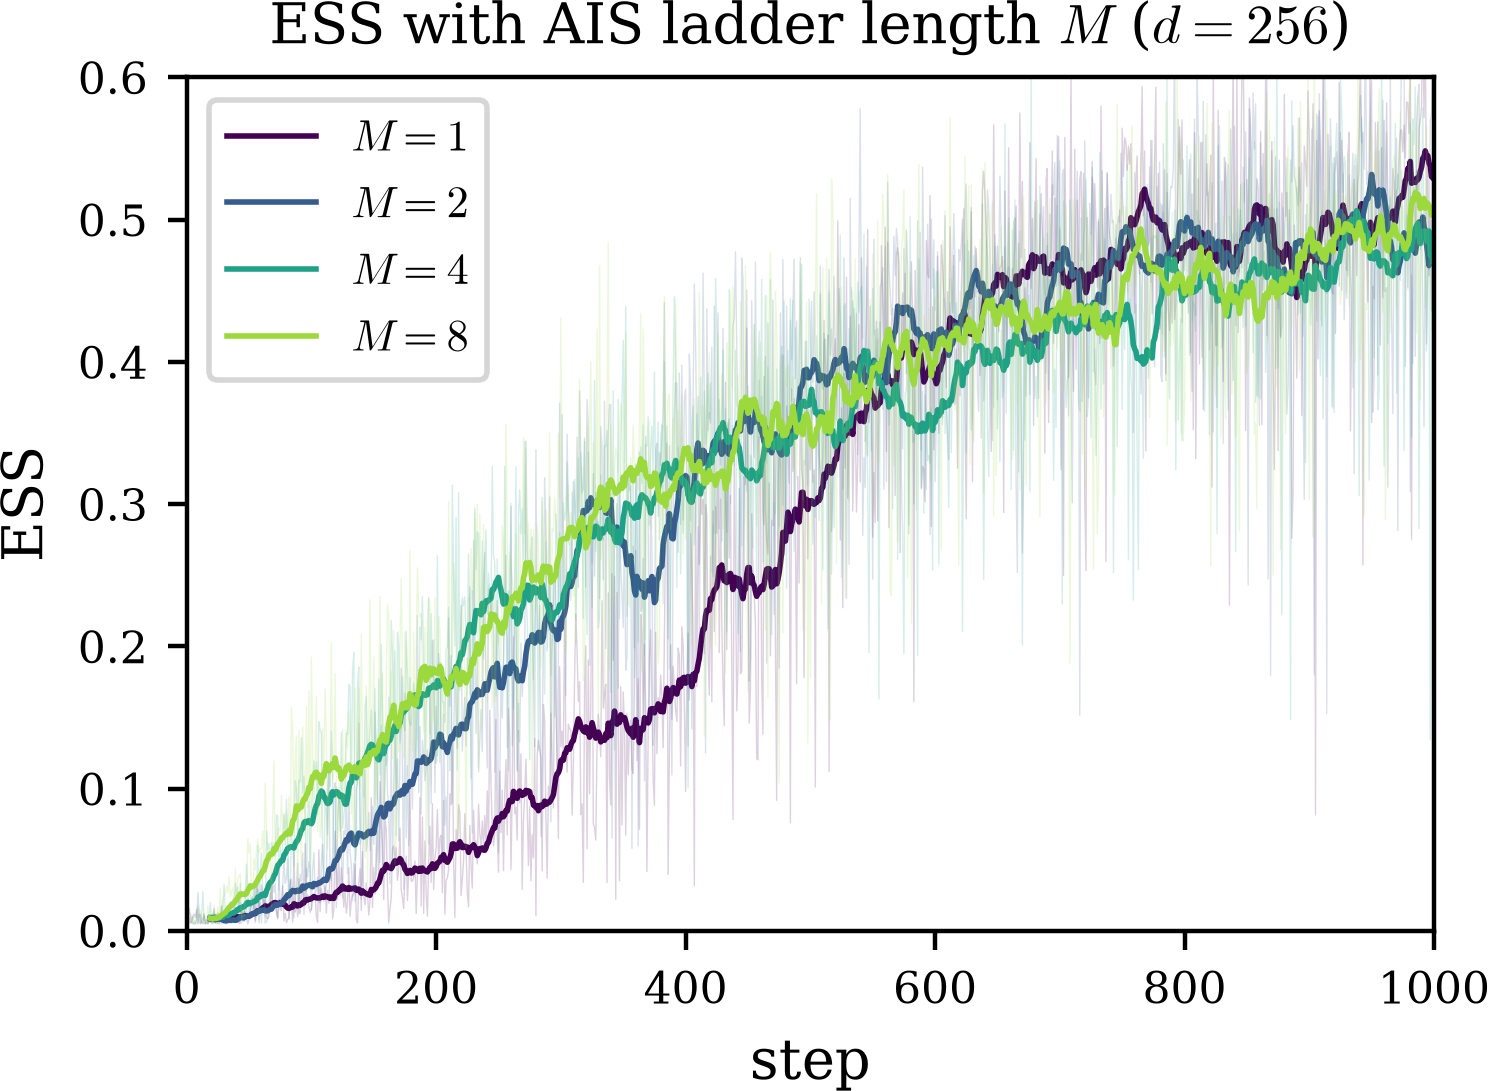
\includegraphics[width=0.45\textwidth]{figures/HD_Product_Ladder/ESS_ladder.png}
    \caption{ESS trajectory across training steps for the mixture loss $\KL{+}\X_\mu{+}\X_{(\hat\mu+\bar\nu)/2}$ on the product multi-well at $d = 256$, as the AIS ladder length $M$ that builds the $\mu$-surrogate is varied over $\{1, 2, 4, 8\}$. Faint lines are the raw per-step ESS; bold lines are a moving average.}
    \label{fig: highd-ladder}
\end{figure}

\subsection{Lattice \texorpdfstring{$\phi^4$}{phi4} field theory: fake ESS at a collective barrier}
\label{subsec: phi4}

The scalar $\phi^4$ lattice theory is a standard testbed on which flow-based samplers are known to collapse. We use its \emph{tilted} broken phase as a sharp fake ESS instance. The target is the scalar $\phi^4$ field on a periodic $L \times L$ lattice, one real value $\phi_j$ per site, $\boldsymbol{\phi} \in \mathbb R^{d}$ with $d = L^2$, distributed as $\mu \propto e^{-U}$ with action
\begin{equation*}
    U(\boldsymbol{\phi}) = -2\kappa_{\mathrm{lat}} \sum_{\langle j l \rangle} \phi_j \phi_l + \sum_{j=1}^{d} \Big[ \phi_j^2 + \lambda_4\big(\phi_j^2 - 1\big)^2 \Big] + h \sum_{j=1}^{d} \phi_j ,
\end{equation*}
with $\langle j l \rangle$ running over nearest-neighbor pairs. In the broken phase the lattice orders into two aligned states near $\pm v\,\mathbf 1$, the uniform configurations of field value $\pm v$ ($\mathbf 1$ the all-ones vector), separated by a \emph{collective} barrier, the free energy of the domain wall any continuous path between them must build; the order parameter is the magnetization $m(\boldsymbol{\phi}) = \frac{1}{d}\sum_{j=1}^{d} \phi_j$, whose distribution is sharply bimodal. The tilt $h$ breaks the symmetry and carries the design: at $h = 0$ the two vacua hold weight $\frac12$ each \emph{by symmetry}, so a collapsed flow loses nothing that symmetrization cannot restore, and equivariant architectures bypass the failure; with $h \ne 0$ the relative weight $p_+/p_- = e^{-\Delta F}$, with $p_+ = \mathbb P(m > 0)$ the weight of the minority phase, is a nontrivial number that the sampler must reproduce. We report $L = 6$ and $L = 8$. The parameters are frozen by a classical pilot scan: $\lambda_4 = \frac12$ throughout; $\kappa_{\mathrm{lat}} = 0.40$, $h = 0.0257$ at $L = 6$ and $\kappa_{\mathrm{lat}} = 0.40$, $h = 0.0144$ at $L = 8$, placing the measured barrier at $8.0$ and $10.2\,k_B T$ and the minority-phase weight at $p_+ = 0.128$ and $0.139$. The reference is parallel tempering with the Metropolis-adjusted Langevin algorithm (MALA) over an action-scaling ladder, completing $3.7\times 10^3$--$4.9\times 10^4$ ladder round trips per run.

The protocol is the single-flow pipeline of Section~\ref{subsec: 2d-benchmark}, unchanged: a neural spline flow on $[-3,3]^d$ with $6$ coupling transforms, $16$ bins, and hidden widths $(256, 256)$; source $\mathcal N(0, 0.25\, I_d)$ centered on the barrier top; batch size $500$, $2000$ Adam steps at learning rate $10^{-3}$; the $\mu$-surrogate is the one importance-weighted resampling pass followed by $50$ Langevin steps; $\hat\mu$ is built once by QT on $U$, which lands in both vacua from $45$--$51\%$ of melted starts. Training carries a stability guard: a non-finite loss or gradient skips the gradient step under gradient clipping. Single-flow training is deliberate: a large lattice calls for the adaptive-temperature generator of Section~\ref{M-sec: boltzmann}, whose hot rungs mix the vacua by construction and would dissolve the failure under study; this benchmark isolates the regime in which the ESS diagnostic itself is misleading.

\begin{table}[h]
    \centering
    \begin{tabular}{@{}l cc cc@{}}
        \toprule
        & \multicolumn{2}{c}{$L = 6$ ($d = 36$)} & \multicolumn{2}{c}{$L = 8$ ($d = 64$)} \\
        \cmidrule(lr){2-3} \cmidrule(lr){4-5}
        & ESS & $p_+$ & ESS & $p_+$ \\
        \midrule
        forward KL & $0.77 \pm 0.04$ & $0,\,0,\,0$ & $0.57 \pm 0.09$ & $0,\,0,\,1$ \\
        $\KL{+}\X_\mu$ & $0.93 \pm 0.01$ & $0,\,0,\,1$ & $0.81 \pm 0.01$ & $0,\,0,\,1$ \\
        $\KL{+}\X_\mu{+}\X_{\hat\mu}$ & $0.88 \pm 0.01$ & $\mathbf{0.126 \pm 0.001}$ & $0.66 \pm 0.02$ & $\mathbf{0.127 \pm 0.001}$ \\
        $\KL{+}\X_\mu{+}\X_{(\hat\mu+\bar\nu)/2}$ & $0.89 \pm 0.01$ & $\mathbf{0.124 \pm 0.002}$ & $0.68 \pm 0.02$ & $\mathbf{0.127 \pm 0.001}$ \\
        \midrule
        PT reference & --- & $0.128$ & --- & $0.139$ \\
        \bottomrule
    \end{tabular}
    \caption{Final ESS and reweighted minority-phase weight $p_+$ on the tilted $\phi^4$ lattice, three seeds per size; for the collapsed losses the $p_+$ column lists the per-seed outcomes, $1$ denoting collapse onto the \emph{minority} vacuum. Bold marks the recovered phase weights.}
    \label{tab: phi4}
\end{table}

\begin{figure}[t]
    \centering
    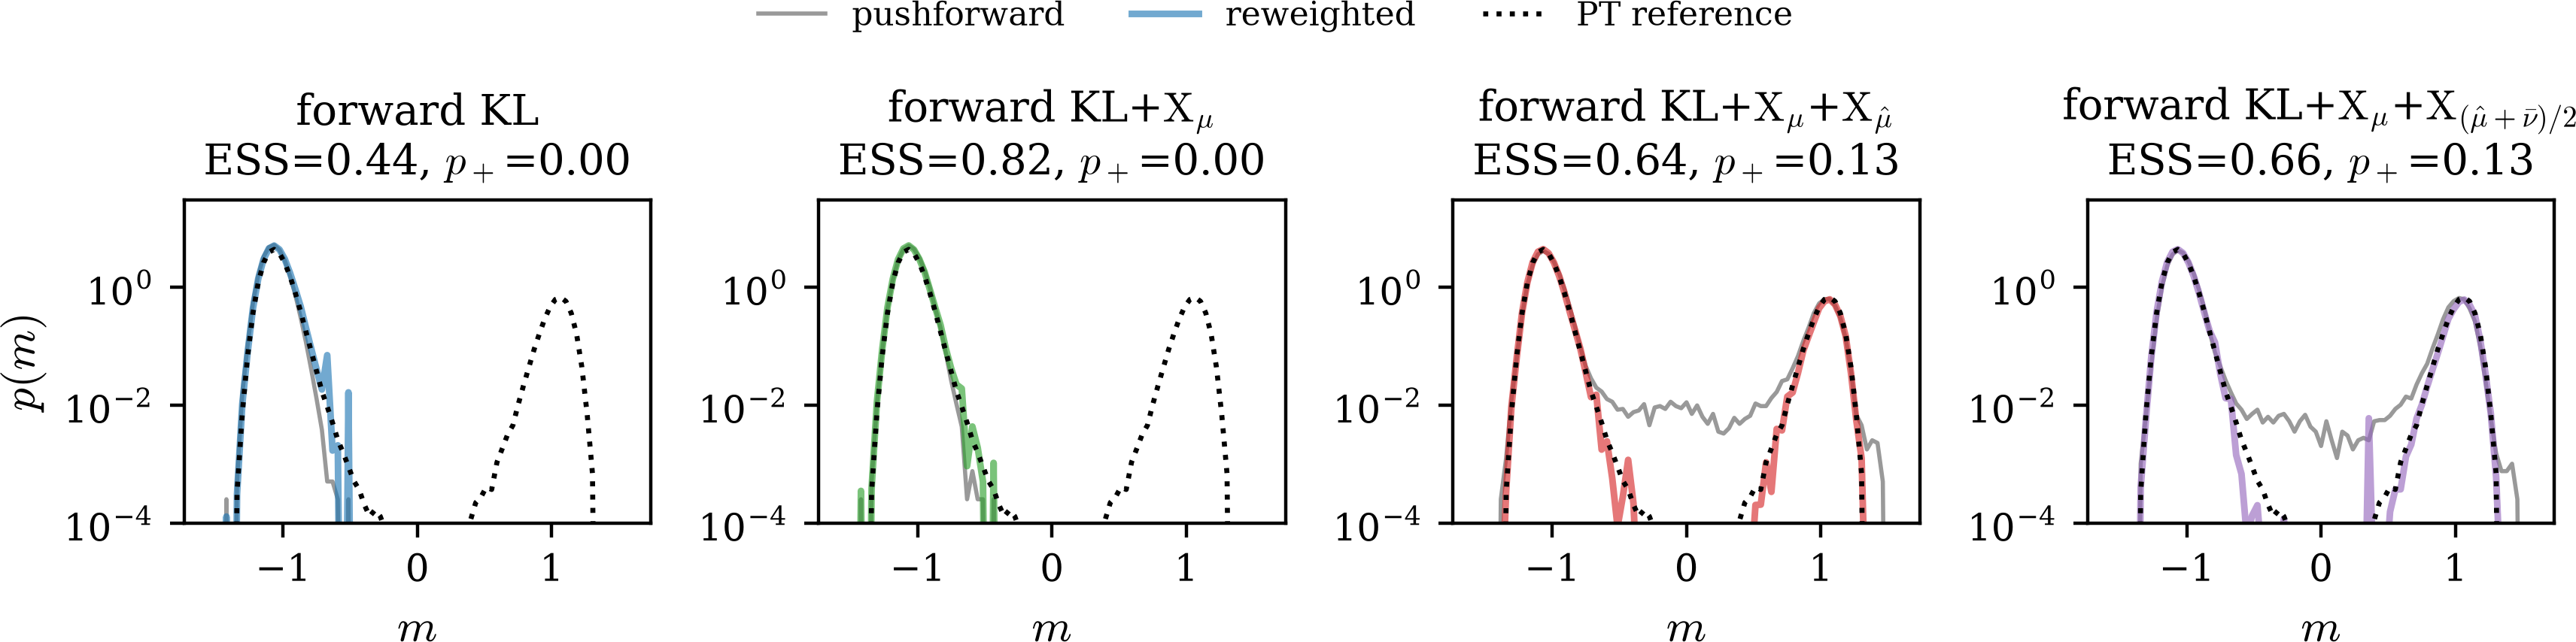
\includegraphics[width=\textwidth]{figures/Phi4_Lattice_8/fig_methods.png}
    \caption{Magnetization density $p(m)$ on the $L = 8$ lattice, one panel per training loss. Each panel shows the pushforward density (gray), the reweighted density (color), and the PT reference (dotted); the title reports the final ESS and the reweighted $p_+$.}
    \label{fig: phi4-methods}
\end{figure}

Table~\ref{tab: phi4} and Figure~\ref{fig: phi4-methods} report the outcome. Bare forward KL and $\KL{+}\X_\mu$ collapse at every size and every seed: the AIS chain initialized at the pushforward cannot cross an $8.0$--$10.2\,k_B T$ collective barrier, so the loss never sees the second vacuum, the reweighted $p_+$ is exactly zero or exactly one, and the estimated $\Delta F$ is infinite where the truth is $+1.8$--$1.9\,k_B T$. The collapse direction is unpredictable across seeds: at $L = 6$ one seed of $\KL{+}\X_\mu$ lands on the \emph{minority} vacuum at a fake ESS of $0.93$, and at $L = 8$ both non-QT-driven losses do so, so $\Delta F$ comes out wrong in \emph{sign}. The fake ESS is high and reproducible, $0.81 \pm 0.01$ over seeds for $\KL{+}\X_\mu$ at $L = 8$, and arises as follows: $\X_\mu$ penalizes the spread of $z$ over the batch, and with every batch confined to one well it sharpens the in-well fit, reducing the weight variance on the captured support; a variance-reducing term applied to a truncated support raises the restricted ESS while doing nothing for coverage. The ESS is thus highest where the collapse is most severe. The QT-driven losses repair both sizes at every seed: $p_+$ lands within $0.012$ of the reference with seed spread at most $\pm 0.002$, the minority well is genuinely well sampled rather than rescued by reweighting, with per-mode ESS near or above $0.50$ at $L = 8$, and the cost over the collapsed runs is modest, ESS $0.66$--$0.68$ against $0.81$. This ESS gap has a topological reading: a diffeomorphism maps the connected Gaussian source to a connected pushforward, visible as the strictly positive gray line across the barrier in Figure~\ref{fig: phi4-methods}, so any flow covering both vacua must thread mass through the inter-phase region where the target is exponentially small; that bridge carries near-zero weights, so a flow covering both vacua has a lower ESS than a collapsed one. A training signal driven by ESS alone would not favor covering both vacua; $\X_{\hat\mu}$ forces the discovery regardless. The repaired weight tracks the action, not the QT set: retraining at $L = 6$ with QT sets deliberately skewed to $5\%$ and $25\%$ minority composition returns $p_+ = 0.124$--$0.128$ throughout, the sample-robustness property of $\X_\omega$ in action. Stability-guard skips are confined to the QT-driven losses ($25\%$ for $\X_{\hat\mu}$, $5\%$ for the mixture at $L = 8$, zero for both collapsed losses), the early-training cost of confronting cross-well log-ratio spreads.

The same pattern persists at larger lattices but weakens: at $L = 12$ the collapsed losses still discard the minority phase while their ESS falls to $0.15$, and the QT-driven losses still cover both phases, recovering $p_+$ to within $0.02$ for $\X_{\hat\mu}$ and $0.07$ for the mixture at ESS $0.01$--$0.06$, correct in kind but expensive and drifting in weight. The fake ESS is therefore most pronounced at moderate size, where it is high enough to mislead; beyond it, single-flow training of either loss family is no longer appropriate and the annealed generator of Section~\ref{M-sec: boltzmann} takes over.

\subsection{Boltzmann generator on \texorpdfstring{$p$}{p}-state clock model}
\label{subsec: clock}

The preceding experiments train a single flow map; this experiment exercises the full adaptive-temperature procedure of Algorithm~\ref{M-alg: boltzmann}, contrasting the X-regularized stage loss \eqref{M-eq: stage-loss} against the bare forward KL through an otherwise identical pipeline. The target is the $p$-state clock model on a periodic $8 \times 8$ square lattice, one angle per site,
\begin{equation}
    U(\boldsymbol{\theta}) = -J \sum_{\langle j l \rangle} \cos(\theta_j - \theta_l) \;-\; h \sum_{j=1}^{d} \cos(p\, \theta_j),
    \qquad \boldsymbol{\theta} \in [-\pi, \pi)^{d}, \quad d = 64,
    \label{eq: clock-potential}
\end{equation}
with nearest-neighbor coupling $J = 1$, $\mathbb{Z}_p$ anisotropy $h = \frac12$, and $p = 6$ clock states; for $p \Ge 5$ the model hosts two Berezinskii--Kosterlitz--Thouless (BKT) transitions enclosing a critical quasi-long-range-ordered phase \citep{jose1977renormalization}. The cold measure $\propto e^{-U}$ splits into $p = 6$ equivalent sectors labeled by the phase of the global magnetization
\begin{equation*}
    m(\boldsymbol{\theta}) = \frac{1}{d} \sum_{j=1}^{d} e^{i \theta_j},
    \qquad
    s(\boldsymbol{\theta}) = \Bigl\lfloor \frac{p \arg m(\boldsymbol{\theta})}{2\pi} \Bigr\rceil \bmod p \;\in\; \{0, \dots, 5\},
\end{equation*}
where $\lfloor \cdot \rceil$ denotes rounding to the nearest integer. The annealing path from the uniform measure to $\mu$ traverses the BKT window, where the correlation length grows rapidly and the six sectors deepen simultaneously. Figure~\ref{fig: clock-target} displays this structure on the trained validation set.

\begin{figure}[t]
    \centering
    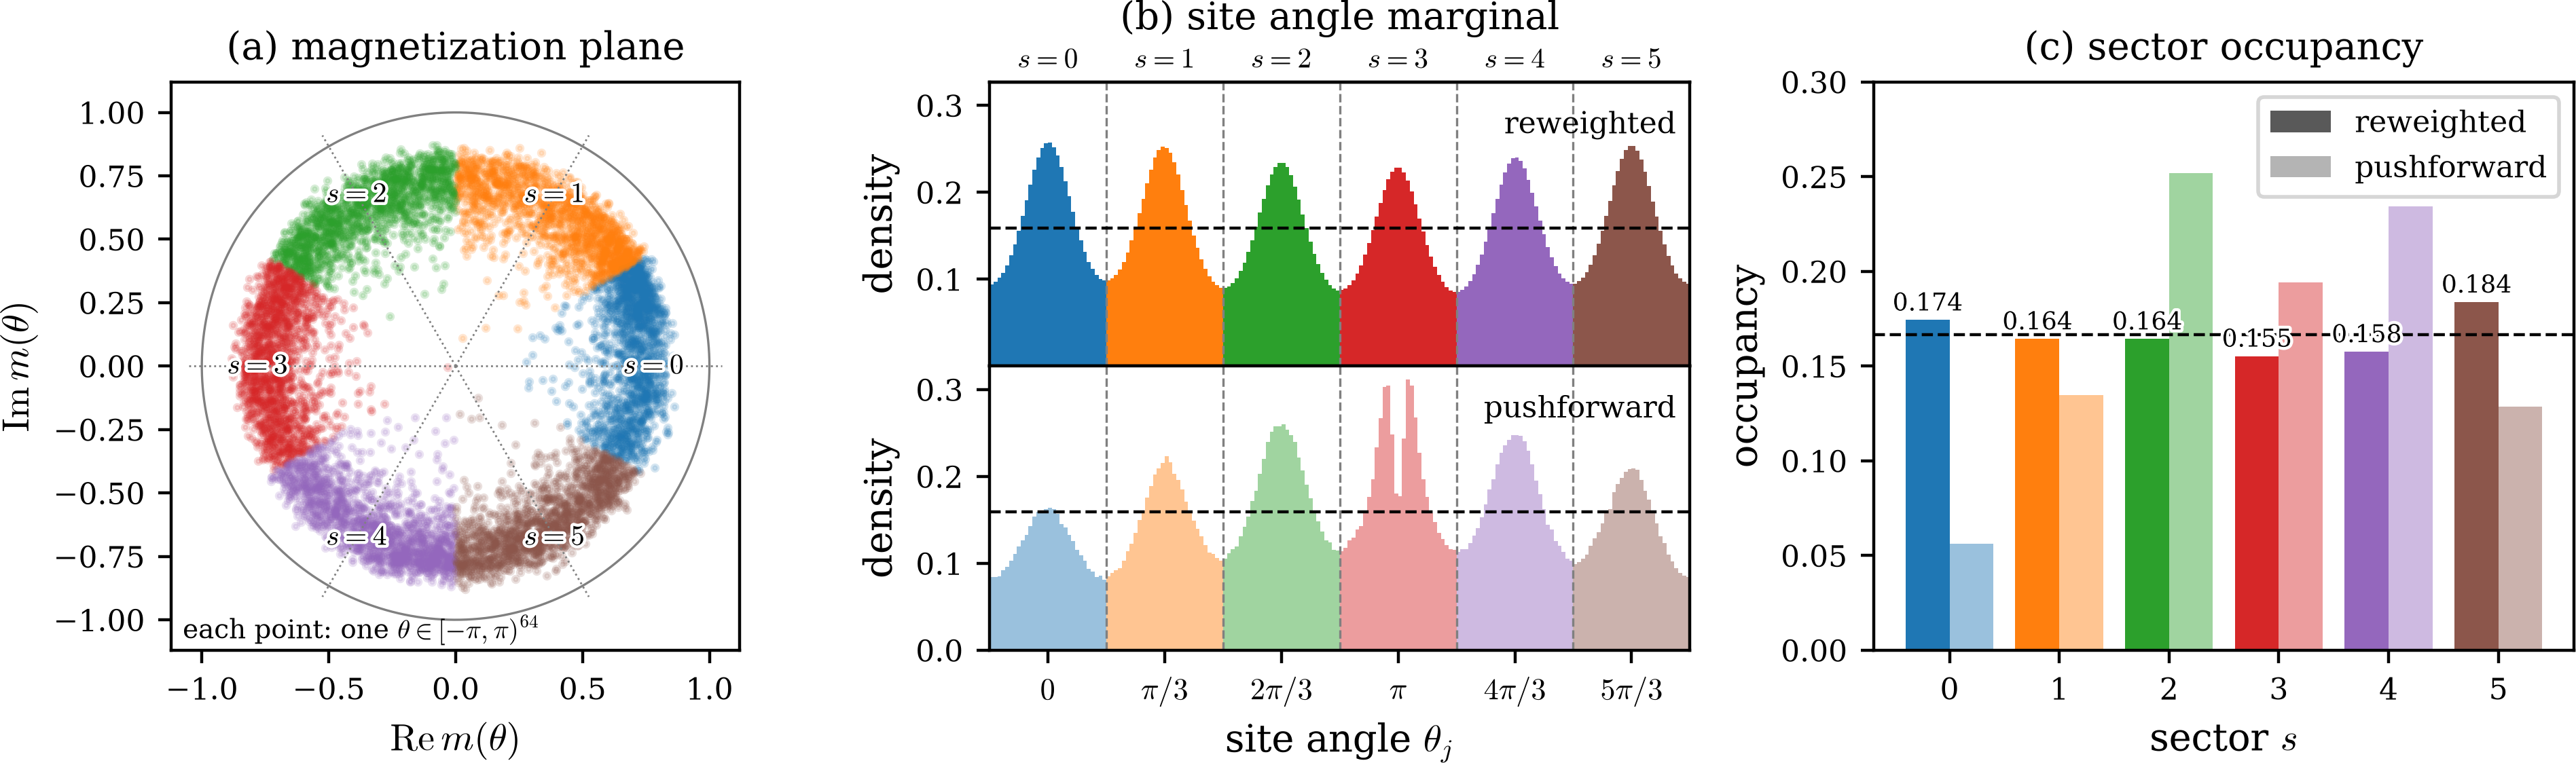
\includegraphics[width=\textwidth]{figures/Clock_Lattice/fig_clock_target.png}
    \caption{Structure of the cold clock measure \eqref{eq: clock-potential} at $d = 64$, displayed on $10^6$ reweighted samples: fresh source draws advanced through the trained ladder by the map--reweight--resample step (v), X-regularized loss at $B = 10^4$. (a) Global magnetization $m(\boldsymbol{\theta})$, colored by sector index $s(\boldsymbol{\theta})$, $1500$ points per sector: the measure splits into $p = 6$ equivalent sectors with mean $|m| = 0.73$. (b) Site-angle marginal: the anisotropy locks each site to the six clock angles $2\pi s/6$, $s = 0, \dots, 5$; dashed lines bound the six wells, colored as in (c), and the black line marks the uniform density $\frac1{2\pi}$; the pushforward marginal is from the maps alone, without reweighting. (c) Sector occupancy of reweighted and pushforward samples, the black line marking the uniform occupancy $\frac16$.}
    \label{fig: clock-target}
\end{figure}

The source is the uniform measure on the torus, $U_0 = 0$, so $U_t = t\, U$; each stage map $G_k$ is a circular neural spline flow on $[-\pi, \pi)^{64}$ with $6$ coupling transforms, $16$ bins, and hidden widths $(256, 256)$. The protocol is deliberately large-sample: a validation set of $10^6$ samples, pool size $P = 2 \times 10^5$, safe start $t_{\mathrm{safe}} = 0.2$, shared ladder length $M = 4$, and SMC floor $\tau = 0.7$, which trims over-aggressive guesses before any training is spent. We report three batch sizes $B = 10^3$, $10^4$, $10^5$, with $2000$, $500$, $200$ Adam steps per stage; the remaining constants are those of Algorithm~\ref{M-alg: boltzmann}. Training carries a stability guard: a non-finite loss skips the gradient step under gradient clipping and a fresh batch is drawn, with a stage abort only after repeated skips. The two losses compared are the full stage loss \eqref{M-eq: stage-loss} at the balanced hyperparameters $\lambda = 1$, $\alpha = \beta = \frac12$, and the bare forward KL, its first term alone; everything else is shared.

Table~\ref{tab: clock-ladder} reports the core metric, the validation ESS of step (v) on every accepted rung. Both losses complete the ladder at every batch size, along \emph{identical} ladders with \emph{identical} rejected rungs: the adaptive machinery converts loss quality into schedule, not into success or failure. Figure~\ref{fig: clock-curves} shows the per-step training ESS on the first three stages. The discrimination lives in the per-rung quality. On accepted rungs the X-regularized loss posts the higher validation ESS on stages 1--3 at all three batch sizes, $+0.21/+0.13/+0.10$ at $B = 10^3$, $+0.17/+0.11/+0.03$ at $B = 10^4$, $+0.13/+0.09/+0.04$ at $B = 10^5$; the gap closes to zero in the transition window, slightly reversing on a few late rungs. Wall time per pair is equal within $3\%$, X-regularized versus bare: $51.9$ versus $50.7$ minutes at $B = 10^3$, $35.7$ versus $34.8$ at $B = 10^4$, and $125.5$ versus $122.8$ at $B = 10^5$; every attempted rung trains the same number of Adam steps, so a rung costs the run average of $3.4$, $4.4$, and $15.5$ minutes respectively, over $15$, $8$, and $8$ attempted rungs. A generalization check pushes $10^6$ independent source samples through the trained $B = 10^4$ ladders, stage by stage with the resampling of step (v): the fresh-sample per-stage ESS tracks the accepted-rung validation ESS of Table~\ref{tab: clock-ladder} within $0.02$--$0.10$ for both losses, and the final sector occupancy is uniform to $\pm 0.02$ per sector, total variation $0.025$, so the gates measure generalization rather than memorization of the carried set.

\begin{table}[h]
    \centering
    \begin{tabular}{@{}c cccccccc@{}}
        \toprule
        stage $k$ & 1 & 2 & 3 & 4 & 5 & 6 & 7 & 8 \\
        \midrule
        $t_k$ \;($B = 10^3$) & $0.200$ & $0.396$ & $0.530$ & $0.662$ & $0.753$ & $0.841$ & $0.952$ & $1.000$ \\
        \midrule
        \multicolumn{1}{@{}l}{forward KL} & $0.391$ & $0.398$ & $0.463$ & $0.366$ & $0.467$ & $\mathbf{0.465}$ & $\mathbf{0.400}$ & $0.708$ \\
        \multicolumn{1}{@{}l}{$\KL{+}\X_\mu{+}\X_{(\hat\mu+\bar\nu)/2}$} & $\mathbf{0.602}$ & $\mathbf{0.524}$ & $\mathbf{0.559}$ & $\mathbf{0.401}$ & $\mathbf{0.500}$ & $0.453$ & $0.369$ & $\mathbf{0.778}$ \\
        \midrule
        $t_k$ \;($B = 10^4$) & $0.200$ & $0.396$ & $0.588$ & $0.720$ & $0.849$ & $1.000$ & --- & --- \\
        \midrule
        \multicolumn{1}{@{}l}{forward KL} & $0.531$ & $0.523$ & $0.347$ & $0.396$ & $\mathbf{0.349}$ & $\mathbf{0.341}$ & --- & --- \\
        \multicolumn{1}{@{}l}{$\KL{+}\X_\mu{+}\X_{(\hat\mu+\bar\nu)/2}$} & $\mathbf{0.703}$ & $\mathbf{0.628}$ & $\mathbf{0.381}$ & $\mathbf{0.412}$ & $0.336$ & $0.303$ & --- & --- \\
        \midrule
        $t_k$ \;($B = 10^5$) & $0.200$ & $0.396$ & $0.588$ & $0.720$ & $0.849$ & $1.000$ & --- & --- \\
        \midrule
        \multicolumn{1}{@{}l}{forward KL} & $0.611$ & $0.602$ & $0.416$ & $0.461$ & $0.400$ & $\mathbf{0.387}$ & --- & --- \\
        \multicolumn{1}{@{}l}{$\KL{+}\X_\mu{+}\X_{(\hat\mu+\bar\nu)/2}$} & $\mathbf{0.745}$ & $\mathbf{0.688}$ & $\mathbf{0.451}$ & $\mathbf{0.489}$ & $\mathbf{0.405}$ & $0.383$ & --- & --- \\
        \bottomrule
    \end{tabular}
    \caption{Validation ESS on every accepted rung, the acceptance gate of Algorithm~\ref{M-alg: boltzmann} with floor $\tau_{\mathrm v} = 0.3$, on the $p = 6$ clock model at $d = 64$; bold marks the better loss on each rung. Within each pair the two losses traverse the same accepted ladder and reject the same rungs, seven rejections per run at $B = 10^3$ and two at $B = 10^4$ and $10^5$.}
    \label{tab: clock-ladder}
\end{table}


\begin{figure}[t]
    \centering
    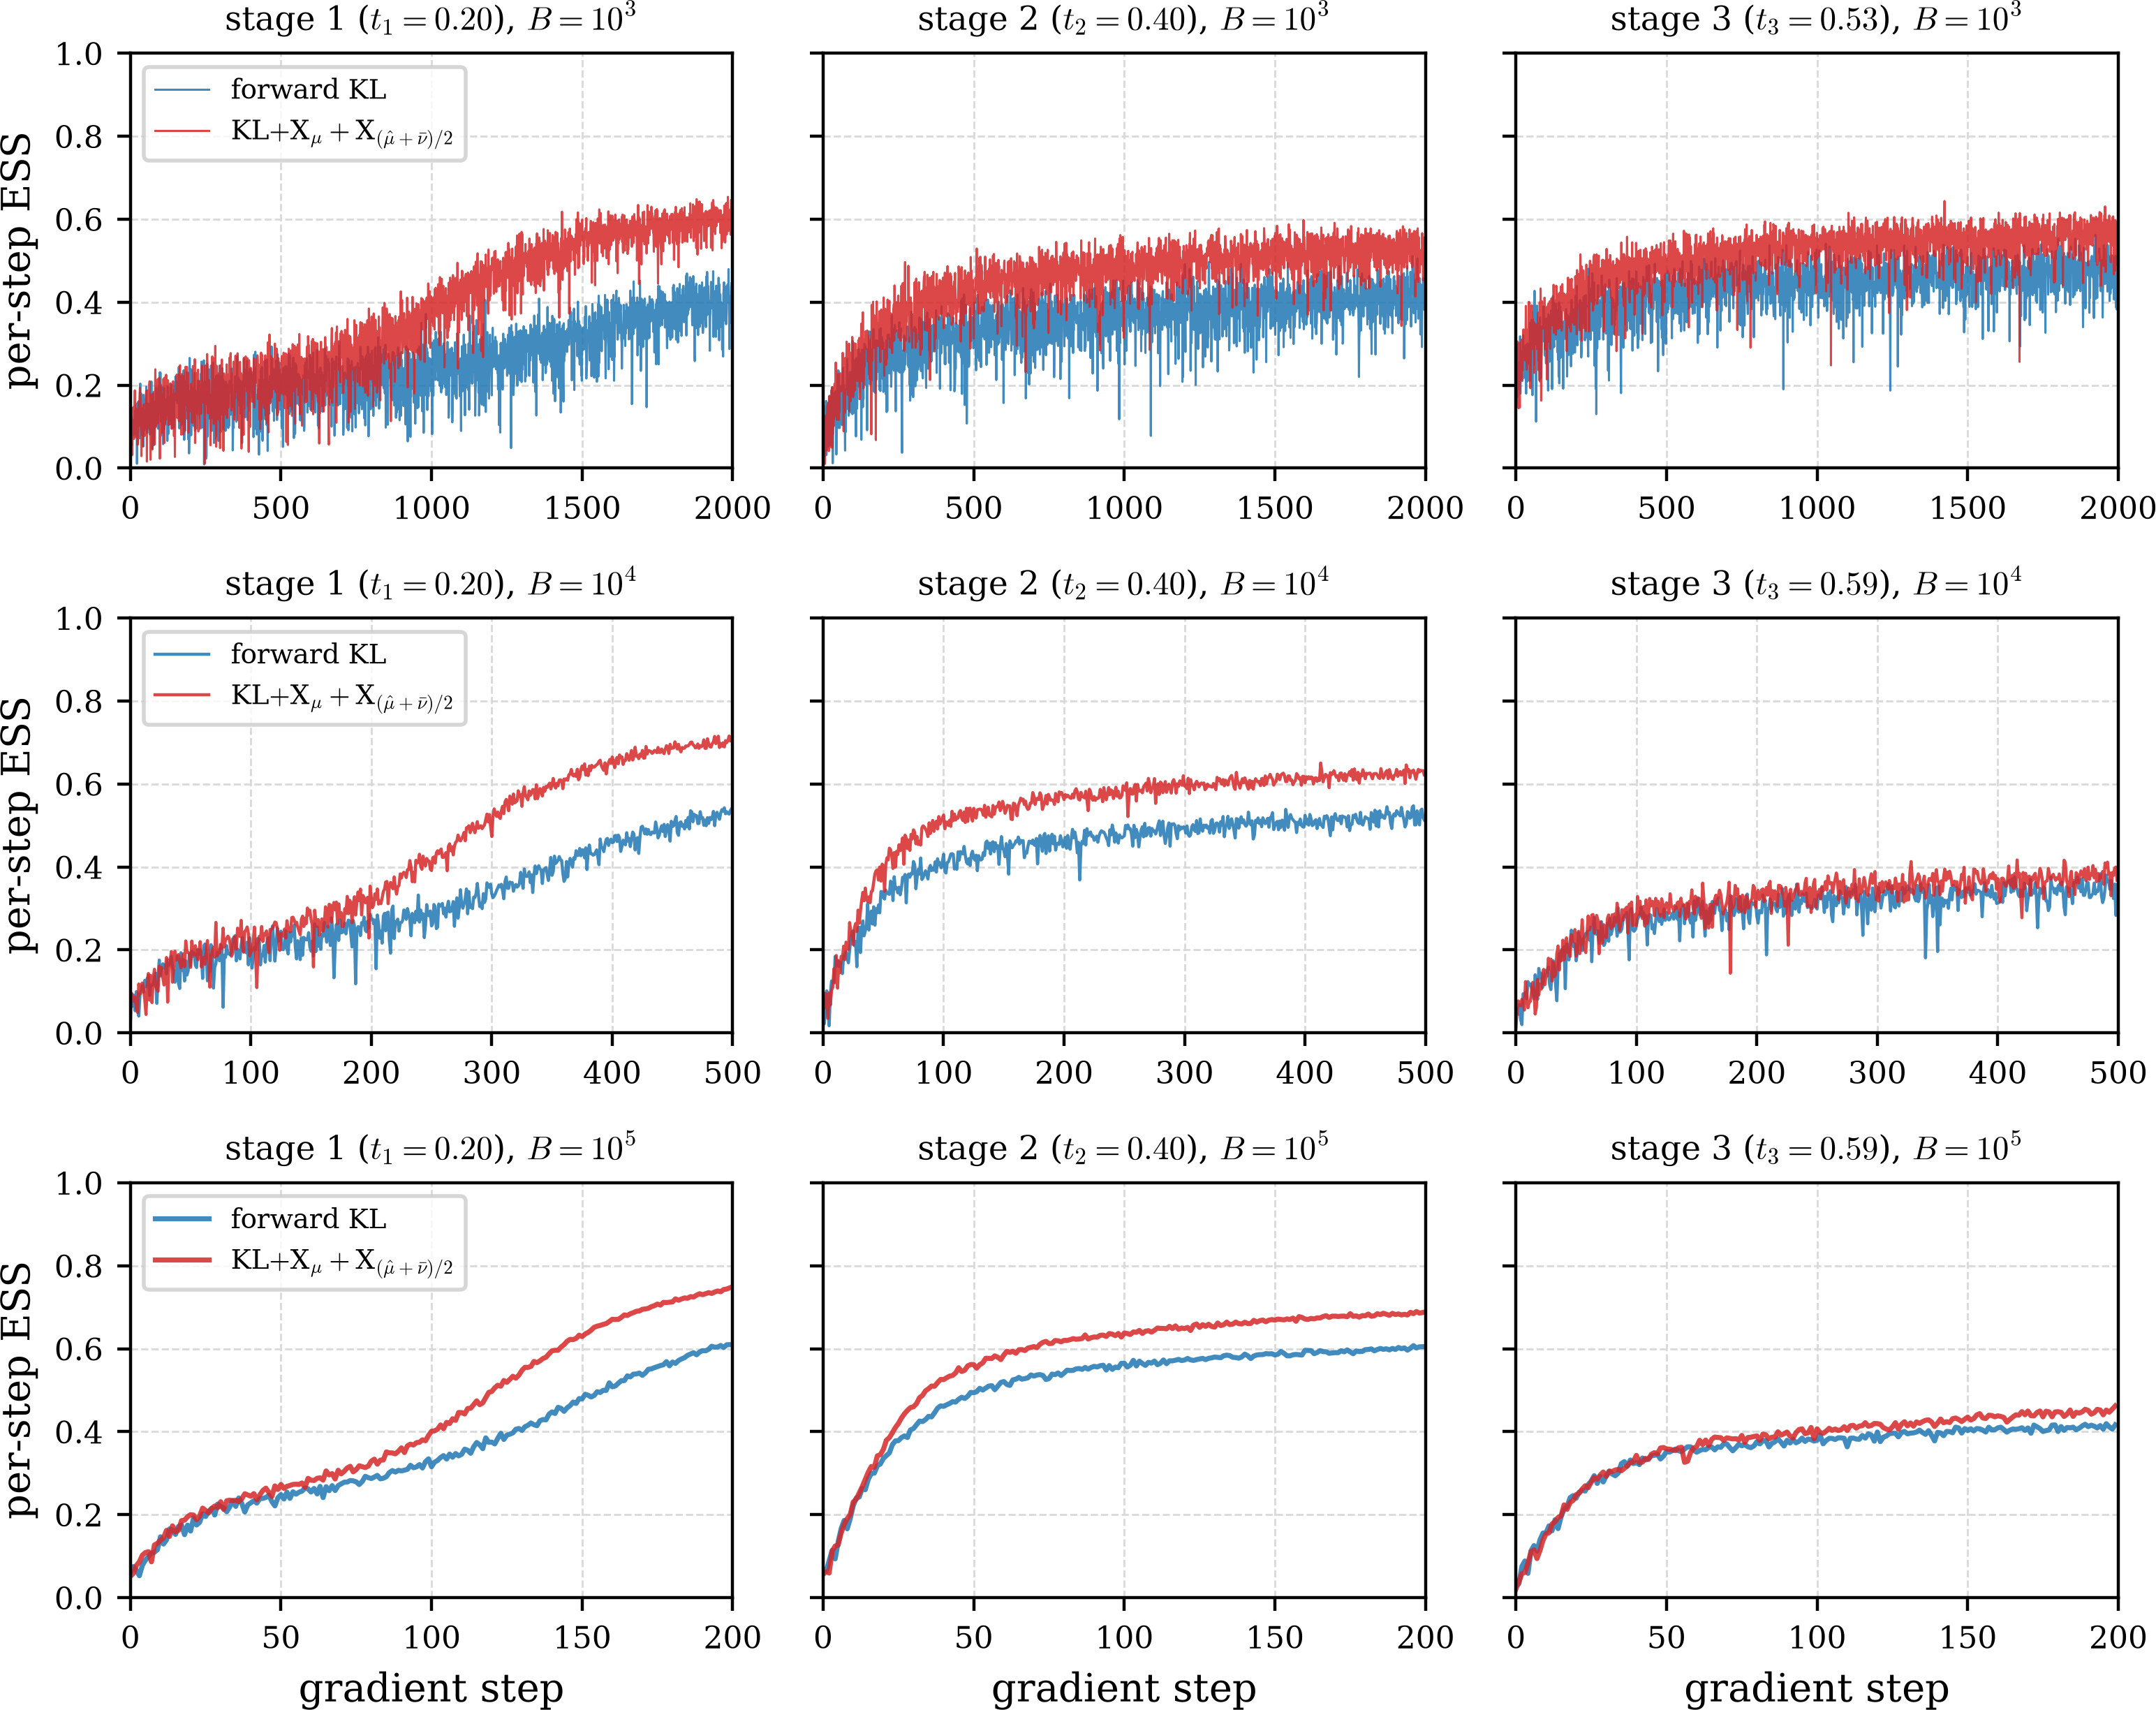
\includegraphics[width=\textwidth]{figures/Clock_Lattice/fig_clock_esscurves.png}
    \caption{Per-step ESS of the training surrogate on the first three stages, bare forward KL (blue) versus the X-regularized loss (red); rows $B = 10^3$, $10^4$, $10^5$, one panel per stage.}
    \label{fig: clock-curves}
\end{figure}

The pattern is consistent with the theory: the X terms lower the asymptotic accuracy floor of each stage (Section~\ref{subsec: accuracy}), a larger training \emph{limit}, but promise no faster transient, and the rejected-rung values confirm that the bare forward KL trains no slower. The anatomy of the ladder shows where the gain lives. The early bridges, $t \Le 0.66$, are far but smooth: a large, structurally simple deformation with a clean AIS signal, so the training loss is the binding constraint and the X terms win by up to $+0.21$. In the transition window, $t \approx 0.66$--$0.95$, the selector halves the accepted increment, an empirical readout of the annealing bottleneck at the BKT crossing; there the ceiling is set by the critically slow Langevin rejuvenation and the shared network capacity, constraints common to both losses, so the gap collapses to zero. The final hop to $t = 1$ is the easiest rung for both. On this target the six sectors are never isolated (Figure~\ref{fig: clock-target}(a)), so the mode discovery channel of $\X_{\hat\mu}$ is not load-bearing; the qualitative separations of Sections~\ref{subsec: 2d-benchmark}--\ref{subsec: highd}, where modes are isolated by construction, do not transfer to soft multimodality. What transfers is a net per-rung quality improvement, concentrated on the early bridges, at zero extra cost: the X-regularized loss was never worse than the bare forward KL where it mattered and never failed where the bare loss passed.

The trained ladder is used as a staged sampler: each stage applies its map $G_k^{-1}$ and then reweights and resamples as in step (v), and Figure~\ref{fig: clock-target}(c) shows the resulting occupancy, uniform to $\pm 0.02$. The residual is nonetheless well above the i.i.d. multinomial floor of $3 \times 10^{-4}$ at $10^6$ samples. The weights of step (v) are pointwise density ratios, exchangeable within a sector and hence sector-blind: they neither detect the imbalance, seeded by the slight flow bias that the i.i.d. pushforward exposes, nor correct it; the cold Langevin rejuvenation transports no mass between sectors; and the final validation set is resampled, carrying no weights at all. The occupancy is thus unbiased in expectation over runs but unrestored within any single one, and the per-stage fluctuations accumulate along the ladder. A scaling test quantifies the accumulation: rebuilding fresh sample sets of size $N = 10^4 \cdot 2^k$, $k = 0, \dots, 7$, through the trained $B = 10^4$ ladder, with $2^{7-k}$ independent rebuilds per size, the mean occupancy bias $\frac{1}{6}\sum_{s}|p_s - \frac16|$ contracts from $0.075$ at $N = 10^4$ to $0.017$ at $N = 1.28 \times 10^6$ at the fitted rate $N^{-0.34}$, shown in Figure~\ref{fig: clock-occbias}, distinctly slower than the Monte Carlo rate $N^{-1/2}$ of a single multinomial draw: the staged sampler composes six map--reweight--resample steps, and each resampling correlates the surviving lineages, so the effective number of independent sector draws grows sublinearly in $N$. Coverage, ESS, and occupancy evenness are three distinct axes of sample quality; the failure that no post-processing could repair, a \emph{missing} sector, does not occur for either loss.

\begin{figure}[t]
    \centering
    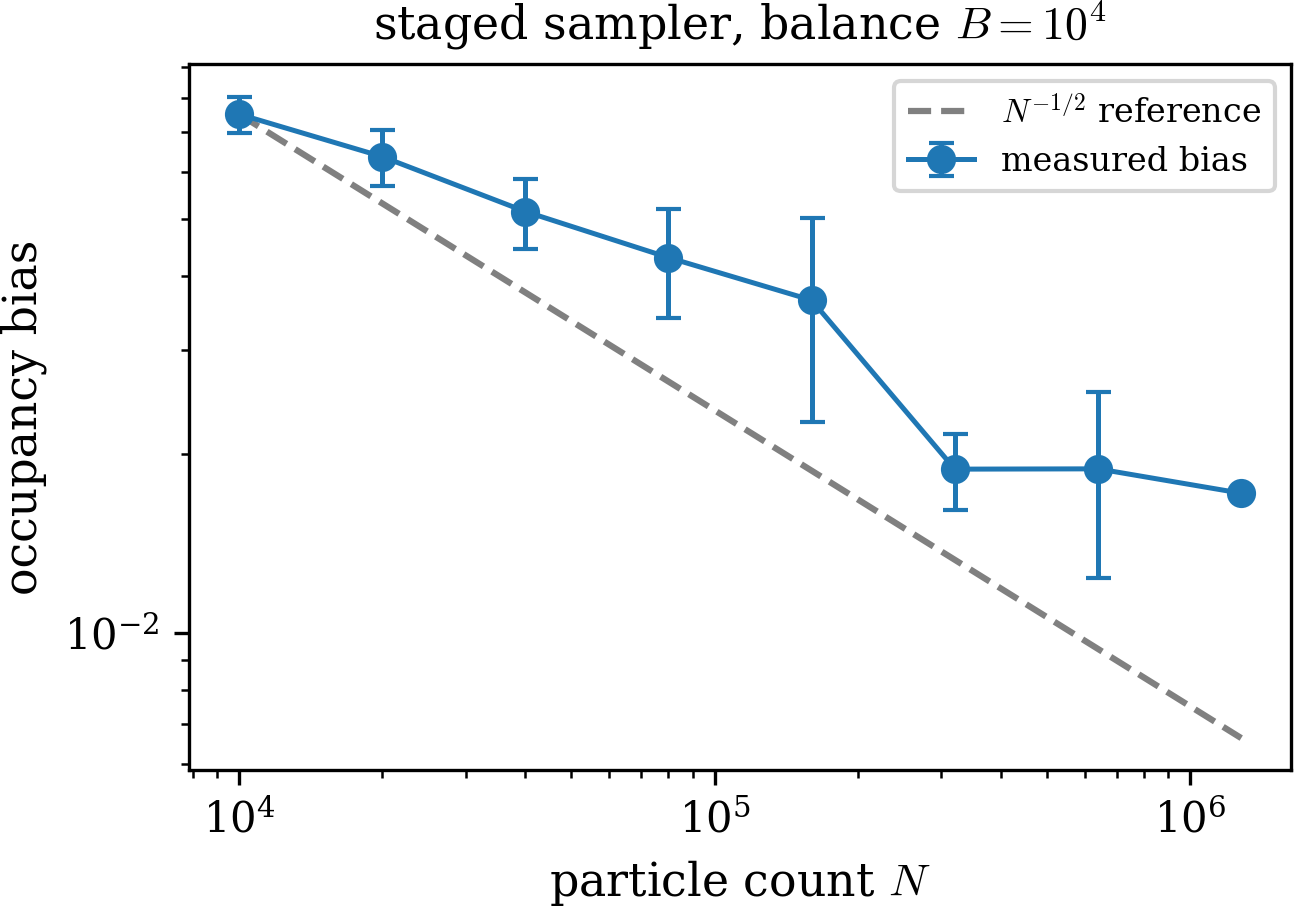
\includegraphics[width=0.5\textwidth]{figures/Clock_Lattice/occupancy_bias_B10k.png}
    \caption{Occupancy bias of fresh staged rebuilds through the trained $B = 10^4$ ladder of the X-regularized loss, versus rebuild size $N = 10^4 \cdot 2^k$, $k = 0, \dots, 7$, averaged over $2^{7-k}$ independent rebuilds per size at equal total work; error bars are $\pm 2$ standard errors. The dashed line is the Monte Carlo reference $N^{-1/2}$.}
    \label{fig: clock-occbias}
\end{figure}


\subsection{Bayesian screened Poisson source inversion}
\label{subsec: poisson}

The final experiment applies the adaptive-temperature generator to a Bayesian PDE inverse problem, the hardest target in our suite: a multimodal posterior with an enumerable well structure that the ladder must reproduce with the correct relative weights. The unknown is a periodic field on $[0,1]^2$,
\begin{equation*}
    v(\mathbf{x}; \boldsymbol{\theta}) = \sum_{\mathbf{k}} \theta_{\mathbf{k}}\, \psi_{\mathbf{k}}(\mathbf{x}),
    \qquad
    \mathbf{x} = (x_1, x_2) \in [0,1]^2,
\end{equation*}
where each basis function is attached to a wave vector $\mathbf{k} = (k_1, k_2) \in \mathbb Z^2$: the constant $\psi_{(0,0)}(\mathbf{x}) \equiv 1$ for $\mathbf{k} = (0,0)$, and the pair
\begin{equation*}
    \psi_{\mathbf{k}}(\mathbf{x}) = \sqrt{2}\cos\bigl(2\pi (k_1 x_1 + k_2 x_2)\bigr),
    \qquad
    \psi_{\mathbf{k}}(\mathbf{x}) = \sqrt{2}\sin\bigl(2\pi (k_1 x_1 + k_2 x_2)\bigr)
\end{equation*}
for every other $\mathbf{k}$, taken once per $\pm \mathbf{k}$ pair over the half-plane $k_1 > 0$ or ($k_1 = 0$, $k_2 > 0$); together these form an orthonormal basis of $L^2([0,1]^2)$. We keep the $d = 36$ Fourier basis functions of smallest $k_1^2 + k_2^2$, an isotropic cutoff. The prior is Gaussian with a steeply decaying spectrum, $\theta_{\mathbf{k}} \sim \mathcal N(0, \sigma_{\mathbf{k}}^2)$ with $\sigma_{\mathbf{k}}^2 = 2/(1 + |\mathbf{k}|^2)^{6}$, so this truncation already captures essentially all of the prior variance. The field drives a screened Poisson equation with a periodic cosine source,
\begin{equation}
    (-\Delta + 25)\, u = 3 \Bigl(1 + \frac12 \cos\bigl(3\, v(\cdot\,; \boldsymbol{\theta})\bigr)\Bigr),
    \label{eq: poisson-forward}
\end{equation}
solved spectrally on a $32 \times 32$ grid, and the observation operator $\mathcal{F}(\boldsymbol{\theta}) = (u(\mathbf{x}_j;\boldsymbol{\theta}))_{j=1}^{54}$ reads the solution $u(\cdot\,;\boldsymbol{\theta})$ of \eqref{eq: poisson-forward} at $54$ sensors on the ring of radius $0.3$ about the center, more sensors than unknowns; Figure~\ref{fig: poisson-setup}(a,b) shows the field $v(\mathbf{x};\boldsymbol{\theta}^\dagger)$ and the observed solution. The observation geometry drives much of the difficulty: all sensors lie on a single small circle, so distinct source configurations produce nearly identical data on the ring, and the posterior concentrates on the resulting family of near-equivalent wells. The data are $\mathbf{y} = \mathcal{F}(\boldsymbol{\theta}^\dagger) + \sigma_{\mathrm{obs}}\, \boldsymbol{\eta}$ with $\boldsymbol{\theta}^\dagger$ a fixed prior draw and $\boldsymbol{\eta}$ standard normal.

\begin{figure}[h]
    \centering
    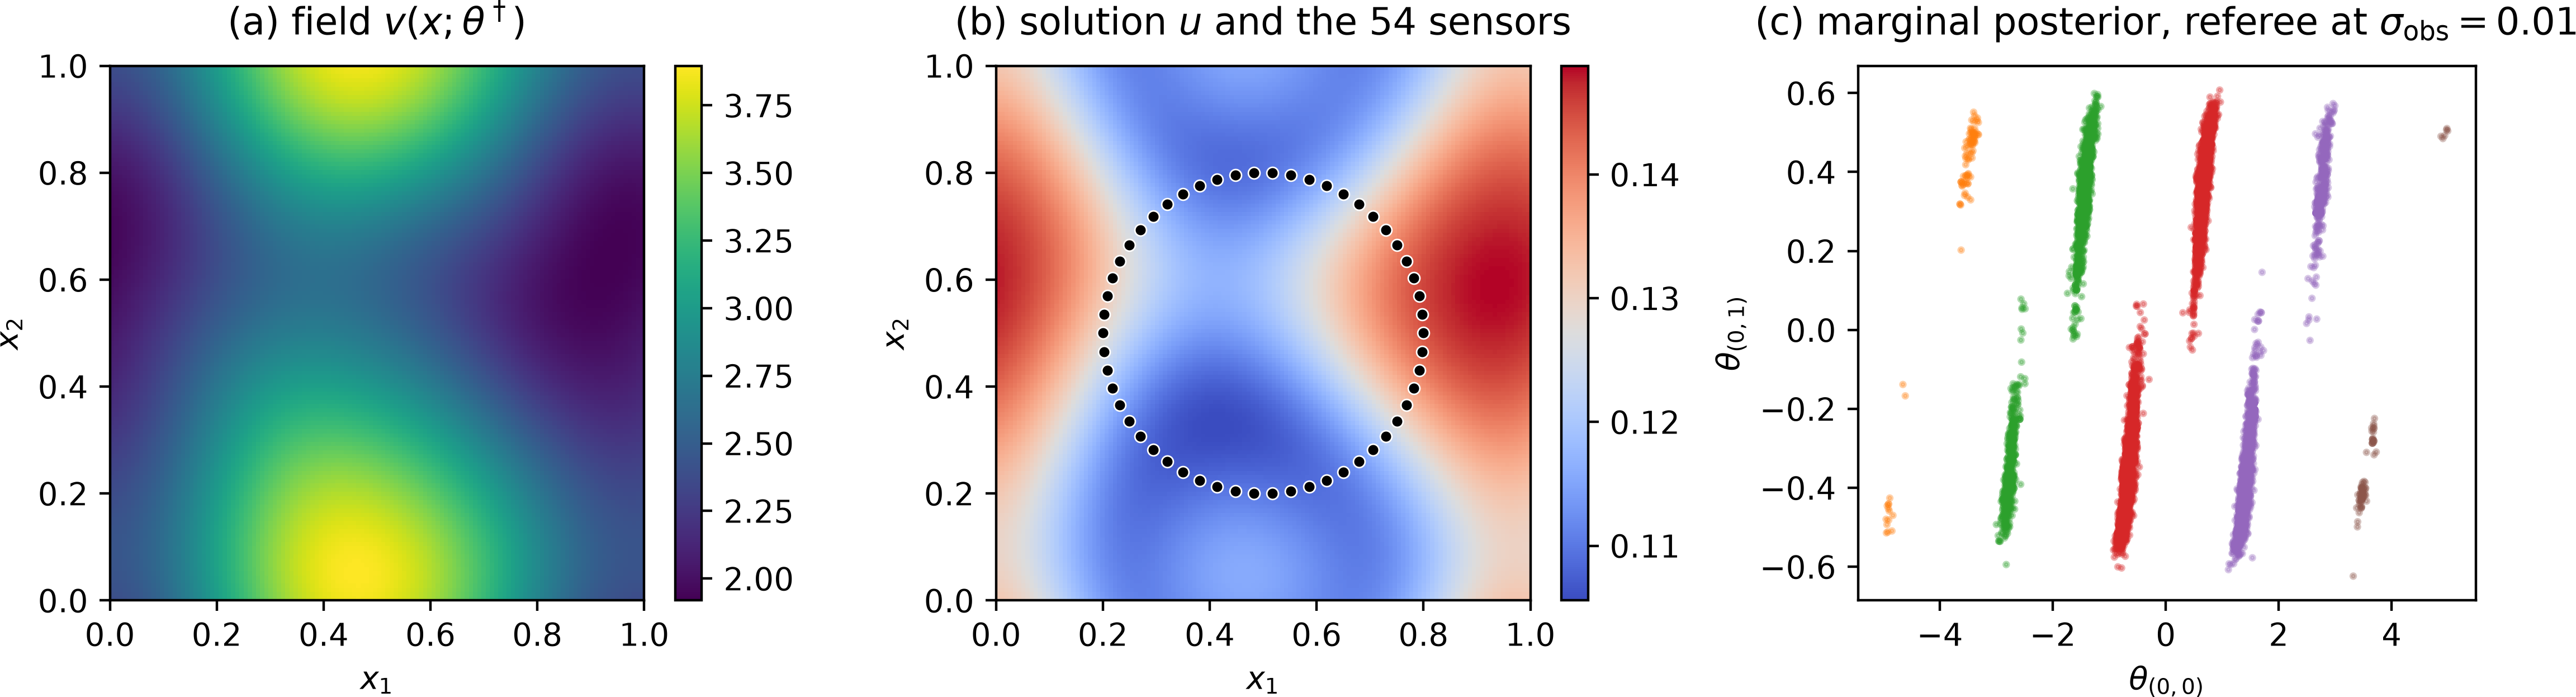
\includegraphics[width=\textwidth]{figures/Poisson_Inverse/fig_setup.png}
    \caption{The screened Poisson inverse problem. (a) The field $v(\mathbf{x};\boldsymbol{\theta}^\dagger)$ on $[0,1]^2$, whose cosine modulation $3(1 + \frac12\cos(3 v(\mathbf{x};\boldsymbol{\theta}^\dagger)))$ is the source. (b) The corresponding solution $u$ of \eqref{eq: poisson-forward} and the $54$ sensors on the ring of radius $0.3$, the dotted circle, where $u$ is observed. (c) The marginal posterior in the coefficients $(\theta_{(0,0)}, \theta_{(0,1)})$ from the parallel tempering referee at $\sigma_{\mathrm{obs}} = 0.01$, colored by the shift index $n$: the posterior splits into the well lattice of the cosine symmetries.}
    \label{fig: poisson-setup}
\end{figure}

All sampling runs on whitened coordinates $\xi_{\mathbf{k}} = \theta_{\mathbf{k}} / \sigma_{\mathbf{k}}$, on which the posterior potential reads
\begin{equation*}
    U(\boldsymbol{\xi}) = \frac12 |\boldsymbol{\xi}|^2 + \Phi(\boldsymbol{\sigma}\odot\boldsymbol{\xi}),
    \qquad
    \Phi(\boldsymbol{\theta}) = \frac{|\mathbf{y} - \mathcal{F}(\boldsymbol{\theta})|^2}{2 \sigma_{\mathrm{obs}}^2},
\end{equation*}
with $\boldsymbol{\sigma} = (\sigma_{\mathbf{k}})$ the vector of prior standard deviations and $\odot$ the element-wise product. The ladder runs with the $d$-dimensional whitened prior as its source, $U_0(\boldsymbol{\xi}) = \frac12|\boldsymbol{\xi}|^2$, so the Algorithm~\ref{M-alg: boltzmann} bridge tempers exactly the likelihood, $(1-t)\, U_0 + t\, U = \frac12|\boldsymbol{\xi}|^2 + t\, \Phi$. The cosine makes the posterior multimodal with an enumerable structure. Writing $\theta_{(0,0)} = \int_{[0,1]^2} v(\mathbf{x};\boldsymbol{\theta})\,\D\mathbf{x}$ for the coefficient of the constant basis function $\psi_{(0,0)} \equiv 1$, the spatial mean of the field, a shift $v \to v + 2\pi n/3$ acts on this mode alone, $\theta_{(0,0)} \to \theta_{(0,0)} + 2\pi n/3$. Since $\cos(3v)$ is invariant under $v \to -v$ and under these shifts, the wells form a lattice indexed by the shift integer $n = \operatorname{round}(3\theta_{(0,0)}/2\pi)$ and a sign, around ten of which carry visible mass, shown in Figure~\ref{fig: poisson-setup}(c). The prior tilts the shift weights and the truth draw tilts the signs, so the well weights are nontrivial numbers. A parallel tempering MALA referee, $20$ temper rungs and $128$ chains certified by $7\,300$--$35\,000$ ladder round trips per noise level, supplies the reference weights.

The ladder runs in dimension $d = 36$; each stage map acts on all $36$ whitened coordinates. Every stage pushes its validation samples through the stage inverse and scores them by the stage importance weight $\log w_k(\boldsymbol{\xi}) = U_{t_{k-1}}(G_k(\boldsymbol{\xi})) - U_{t_k}(\boldsymbol{\xi}) - \log|\det J_{G_k}(\boldsymbol{\xi})|$ of step (v); the ESS of $w$ is the per-stage validation ESS on which the acceptance gate of Algorithm~\ref{M-alg: boltzmann} fires. The protocol is otherwise Algorithm~\ref{M-alg: boltzmann} with NSF stage flows on $[-5,5]^{36}$, batch size $4\,000$, $1\,000$ Adam steps per stage, $M = 6$ surrogate rungs, selection floor $\tau = 0.5$, validation floor $\tau_{\mathrm v} = 0.3$, and at most ten attempts per stage. The observation noise is the difficulty dial: shrinking $\sigma_{\mathrm{obs}}$ sharpens the likelihood by $1/\sigma_{\mathrm{obs}}^2$, deepens the barriers, and widens the annealing gap, leaving the well lattice and the referee intact. We sweep $\sigma_{\mathrm{obs}} \in \{0.01, 0.015, 0.02, 0.025\}$ and run the bare forward KL and the X-regularized stage loss \eqref{M-eq: stage-loss}, $\KL{+}\X_\mu{+}\X_{(\hat\mu+\bar\nu)/2}$ at balanced hyperparameters, on each.

\begin{figure}[h]
    \centering
    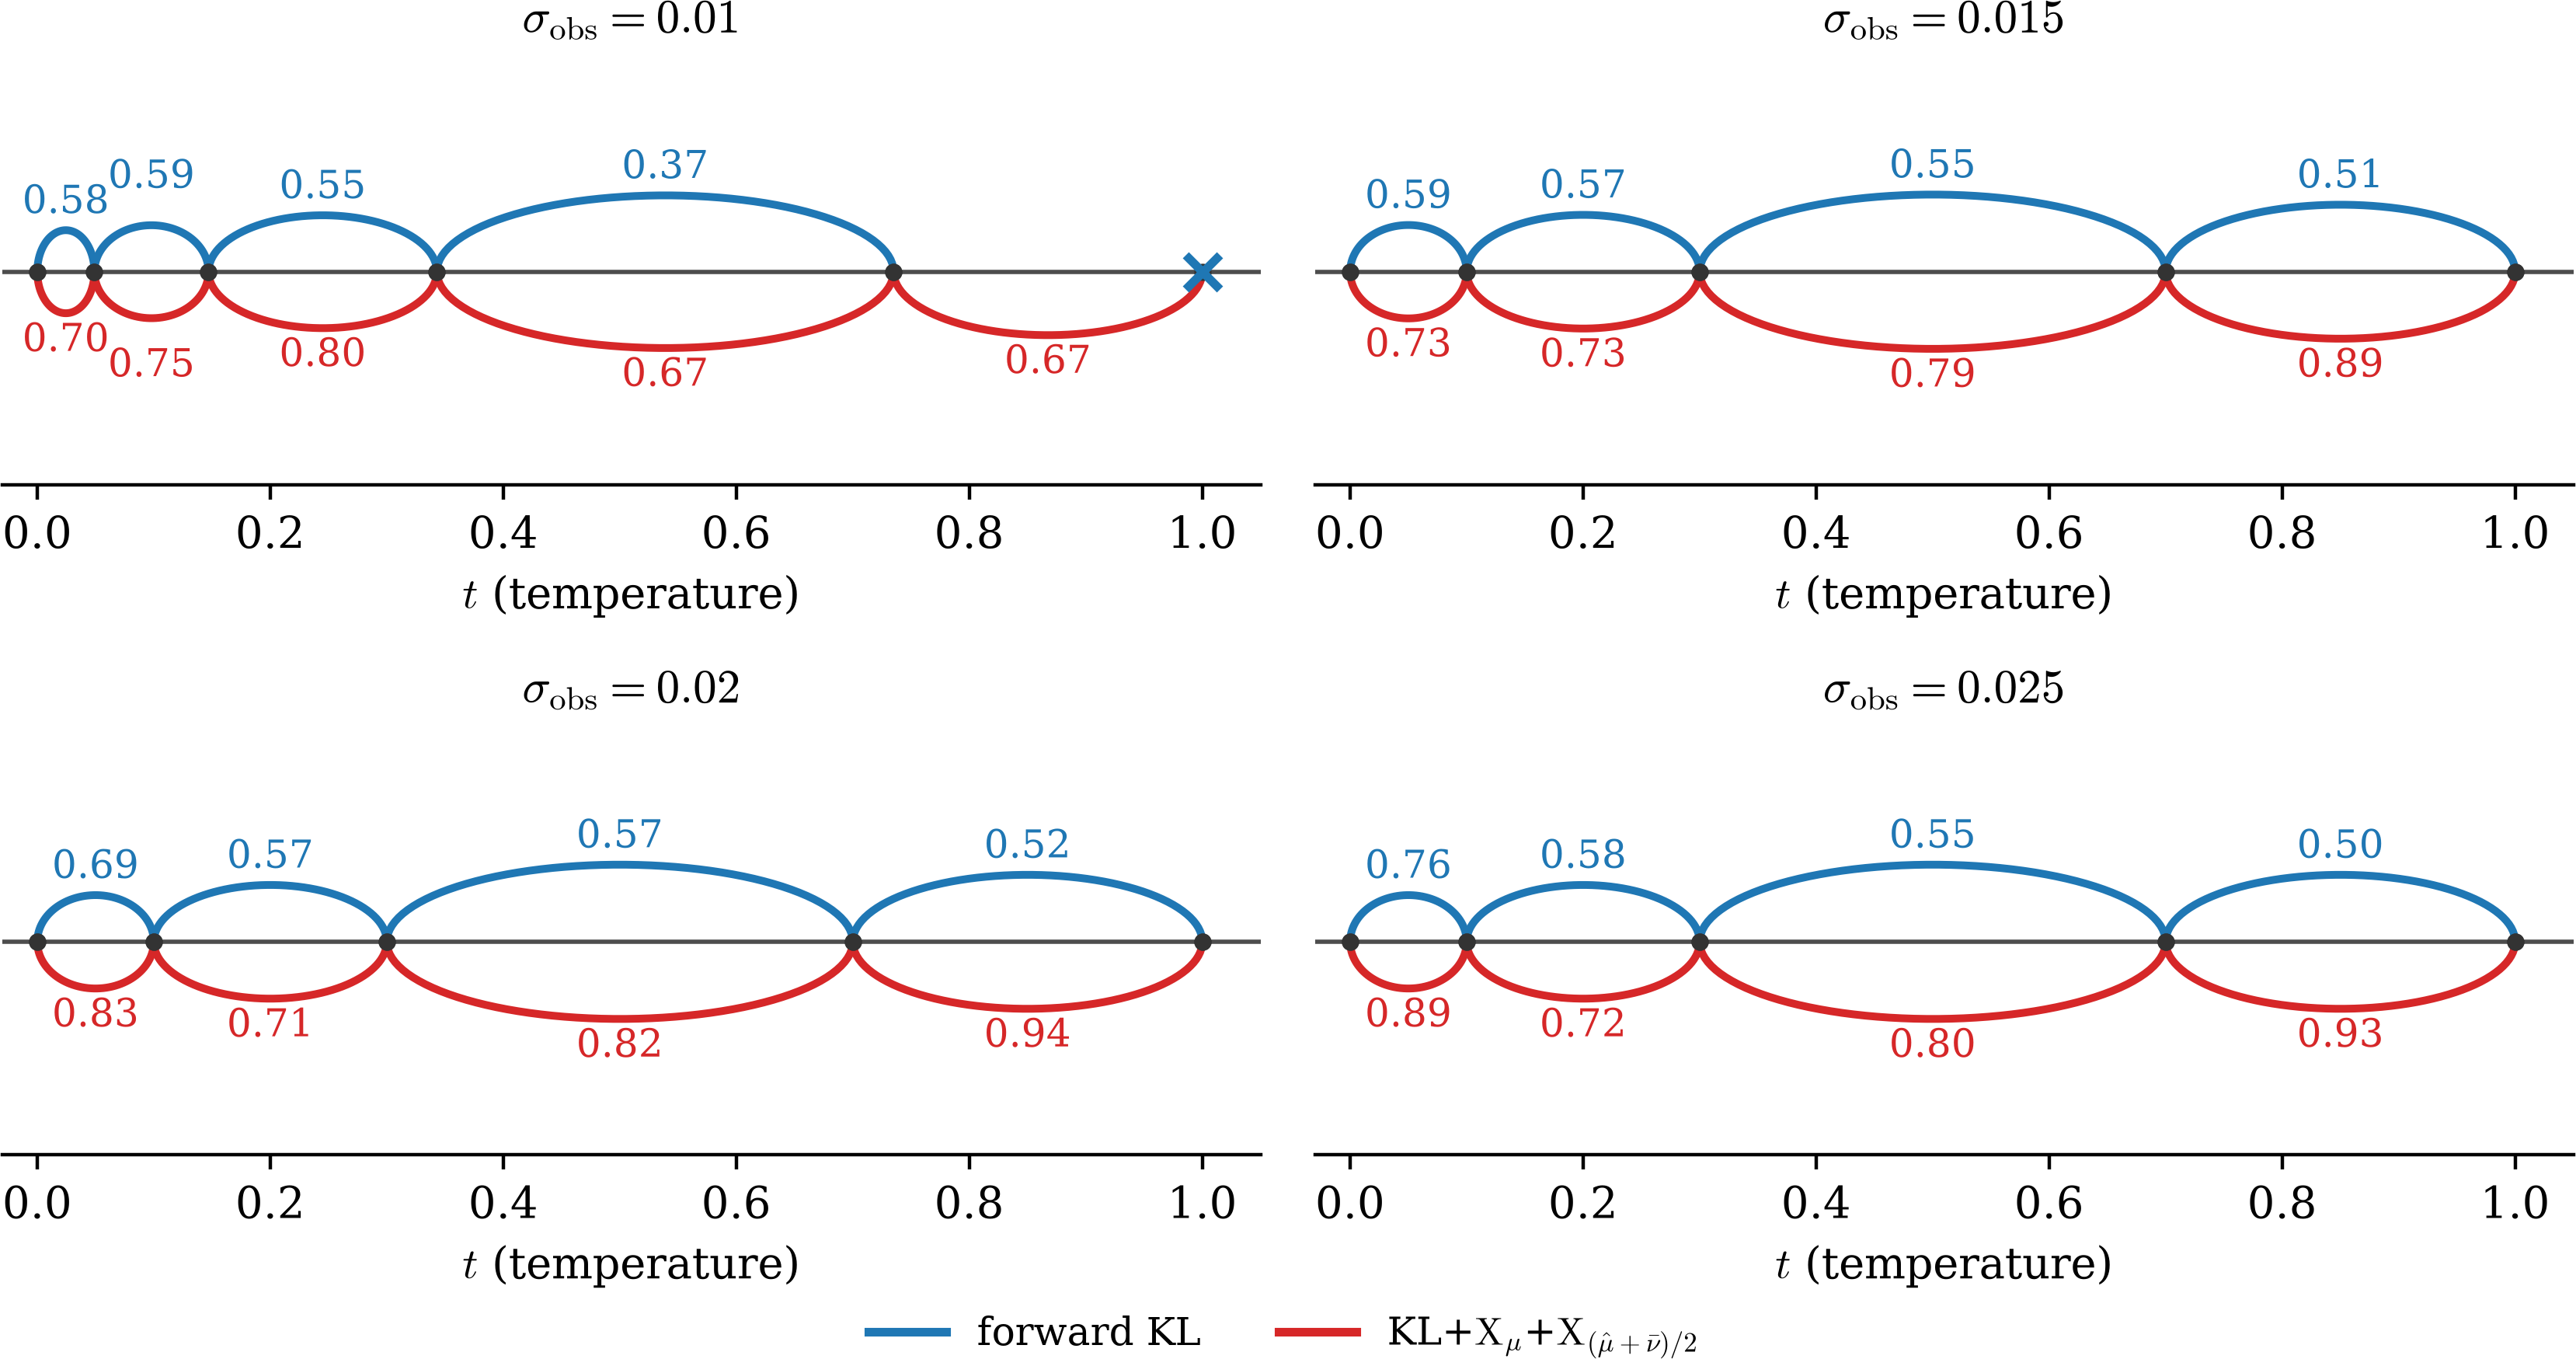
\includegraphics[width=\textwidth]{figures/Poisson_Inverse/poisson_ladders.png}
    \caption{ESS ladders on the screened Poisson posterior across the noise sweep, one panel per $\sigma_{\mathrm{obs}}$. The temperature axis runs $t = 0 \to 1$; each accepted stage is an arc spanning its increment $\Delta t_k$, forward KL above (blue) and the X-regularized loss $\KL{+}\X_\mu{+}\X_{(\hat\mu+\bar\nu)/2}$ below (red), labelled by its per-stage validation ESS. The cross marks the final bridge that the forward KL run failed in all ten attempts at $\sigma_{\mathrm{obs}} = 0.01$. The recovered well weights are reported in Table~\ref{tab: poisson-tv}.}
    \label{fig: poisson-ladders}
\end{figure}

\begin{table}[h]
    \centering
    \small
    \begin{tabular}{@{}c c c@{}}
        \toprule
        $\sigma_{\mathrm{obs}}$ & forward KL & $\KL{+}\X_\mu{+}\X_{(\hat\mu+\bar\nu)/2}$ \\
        \midrule
        $0.010$ & $0.106 \pm 0.039$ & $\mathbf{0.042 \pm 0.002}$ \\
        $0.015$ & $0.077 \pm 0.016$ & $\mathbf{0.041 \pm 0.004}$ \\
        $0.020$ & $0.028 \pm 0.010$ & $\mathbf{0.020 \pm 0.001}$ \\
        $0.025$ & $0.050 \pm 0.004$ & $\mathbf{0.019 \pm 0.003}$ \\
        \bottomrule
    \end{tabular}
    \caption{Total-variation distance of the staged sampler's well weights from the parallel tempering reference, across the noise sweep; mean and spread over three independent replays of the trained ladder. Bold marks the smaller distance of each pair. The forward KL run at $\sigma_{\mathrm{obs}} = 0.01$ did not reach $t = 1$ (Figure~\ref{fig: poisson-ladders}); its weights are read from the last accepted stage.}
    \label{tab: poisson-tv}
\end{table}

Figure~\ref{fig: poisson-ladders} reports the outcome in three layers. First, existence: at the sharpest noise the bare forward KL cannot finish the ladder; its per-stage ESS starts at $0.58$ and falls to $0.37$ on the final accepted rung, and the bridge to $t = 1$ fails all ten retraining attempts, while the X-regularized loss completes the same rungs at $0.67$--$0.80$ in $39$ minutes against $95$ spent failing. Second, per-stage quality: at every noise level the X-regularized loss leads on every rung; on the final rung of the three completed sweeps the X-regularized loss reaches $0.89$--$0.94$ against the forward KL's $0.50$--$0.52$. The separation is considerably larger than on the $p$-state clock model of Section~\ref{subsec: clock}, where both losses completed identical ladders and the X terms improved a rung by at most $+0.21$: the PDE posterior is closer to ill-posedness, its prior-to-posterior gap growing as $1/\sigma_{\mathrm{obs}}^2$, and on such ladders the training signal rather than the sampling physics is the binding constraint, and the X terms are designed to strengthen the training signal. Third, weight accuracy (Table~\ref{tab: poisson-tv}), measured by replaying the trained ladder as the staged sampler of step (v) three times per run: with the gates passed and the ladders complete, the bare forward KL produces well weights at total variation $0.028$--$0.077$ from the certified reference, with a replay spread up to $\pm 0.016$; the X-regularized loss reproduces the reference at $0.019$--$0.042$ with replay spread within $\pm 0.004$, closer and roughly $4\times$ more reproducible, with up to $2.6\times$ smaller total-variation error where the forward KL completes the ladder. A completed ladder with per-stage ESS above the validation floor does not guarantee correct well weights: the per-stage diagnostic is local in temperature and blind to the slow drift of the carried set, an accumulation of the same kind as the occupancy drift of Section~\ref{subsec: clock}, though here it lives in the relative well weights, and only the QT-driven mixture keeps them pinned. The error originates in the carried validation set: each stage resamples it by the trained flow's weights, so a small per-stage bias in the relative well masses propagates into every later stage, and the per-stage ESS does not register it. Both losses cover all ten wells that the referee certifies above the $10^{-3}$ level in every run; the carried validation set preserves the support, and the failure is confined to the density fit and the weights, the regime the $\X_\mu$ and mixture terms address.


% ===================== Section S3: molecular (verbatim main S6) =====================
\section{Boltzmann generators on molecular potential energies}
\label{sec: molecular}

The model problems of the previous section were each chosen to isolate one failure mode of forward KL training
on a smooth target: the 2D benchmarks, the lattice $\phi^4$ theory, and the screened Poisson inversion.
The application that motivates a Boltzmann generator in the first place is a molecule, and a molecular target
exercises the whole pipeline at once. This section applies the adaptive-temperature, X-regularized generator
of the previous section to three molecules of increasing difficulty in full internal coordinates,
$d = 36$ to $60$, on a single consumer GPU. It is organized into five parts: the motivation and the two
difficulties that make a molecular potential hard (Section~\ref{sec: mol-background}); \emph{sharpening}, the core simplification that makes the framework tractable on a singular target (Section~\ref{sec: mol-sharpening}); the
molecule-specific engineering it requires (Section~\ref{sec: mol-engineering}); the numerical results on
glycerol, diethanolamine, and alanine dipeptide (Section~\ref{sec: mol-results}); and the limitations of the
molecular study (Section~\ref{sec: mol-limitations}).

\subsection{Motivation and background}
\label{sec: mol-background}

The distribution that motivates a Boltzmann generator is a molecule: the equilibrium (Boltzmann) distribution
$\mu \propto e^{-U}$ of a molecular potential, with $U$ its dimensionless reduced form, whose samples are the conformers that set binding
affinities, reaction rates, and free energies in computational chemistry and drug design
\citep{noe2019boltzmann}. The targets studied so far were smooth by design; a molecular potential is not. Drawing \emph{independent} samples from
$\mu$ is the central computational problem: MD and MCMC mix slowly across
the high torsion barriers that separate conformers, so a trained flow that emits independent conformers with a
tractable density, and therefore supports the exact importance-sampling pipeline of the previous sections, is
the payoff that justifies the training cost.

We take the potential energy to be the Amber molecular-mechanics force field \citep{cornell1995amber}, the
standard classical model, with raw force-field energy $U_{\mathrm{FF}}(x)$ in kJ/mol, a sum of bonded terms, harmonic bonds and angles and
periodic torsions, and nonbonded Lennard-Jones and Coulomb terms,
\begin{equation}
    U_{\mathrm{FF}}(x) = \!\!\sum_{\text{bonds}}\!\! k_b (r-r_0)^2 + \!\!\sum_{\text{angles}}\!\! k_\theta (\theta-\theta_0)^2
    + \!\!\sum_{\text{torsions}}\!\! \frac{V_n}{2}\big[1+\cos(n\phi-\gamma)\big]
    + \sum_{i<j}\!\bigg[ 4\epsilon_{ij}\bigg(\frac{\sigma_{ij}^{12}}{r_{ij}^{12}} - \frac{\sigma_{ij}^{6}}{r_{ij}^{6}}\bigg) + \frac{q_i q_j}{r_{ij}} \bigg],
    \label{eq: amber}
\end{equation}
the last sum running over nonbonded atom pairs, with charges in units that absorb the Coulomb constant. The
Boltzmann distribution at temperature $T$ is $\mu \propto e^{-U}$ in the dimensionless reduced potential
\begin{equation*}
    U(x) = \frac{1}{k_B T} U_{\mathrm{FF}}(x),
\end{equation*}
with $k_B$ the Boltzmann constant. We evaluate $U_{\mathrm{FF}}$ for the \emph{isolated
molecule in vacuum}, with no solvent and no nonbonded cutoff; this and two further simplifications of the
molecular study are stressed in Section~\ref{sec: mol-limitations}.

We work in \emph{whitened internal coordinates} \citep{noe2019boltzmann}. The six rigid-body degrees of
freedom, global translation and rotation, leave $U$ unchanged, so we drop them and describe the shape by
bond lengths, bond angles, and torsions, a z-matrix giving a smooth, invertible map $x \mapsto \xi \in
\mathbb R^{d}$ with $d = 3N - 6$ for an $N$-atom molecule and a tractable volume Jacobian. Bonds and angles are stiff and near-Gaussian
about their equilibria, so each is standardized to unit variance; torsions stay periodic on $[-\pi,\pi)$. The
source $\mu_0 \propto e^{-U_0}$ is then a trivial product base, standard normal on the bond/angle
directions and uniform on the torsions, and the target, pulled back through the change of variables, is
\begin{equation*}
    \mu(\xi) \propto \exp\!\big(\!-U(x(\xi))\big)\big|\det\big(\partial x/\partial \xi\big)\big|,
\end{equation*}
so $U_0$ and $U$ as functions of $\xi$ already absorb the change-of-variables log-Jacobian. This is what
makes the target tractable for a flow: the rigid-body symmetries and the stiff, strongly correlated
bond/angle vibrations are factored out, leaving the combinatorially multimodal torsional landscape, the
conformers, as the structure the diffeomorphism must actually transport.

Two features make \eqref{eq: amber} qualitatively harder than a smooth model target, and they compound. First,
the dimension grows with the molecule ($d = 36$ to $60$ here), and the conformer landscape is
\emph{combinatorially multimodal}: every rotatable torsion is multi-well (gauche$^{\pm}$/trans), so the joint
over several torsions has dozens of basins the flow must discover. Second, and more consequential, the
Lennard-Jones $r^{-12}$ repulsion makes $U$ \emph{singular}: as any pair distance $r_{ij} \to 0$ the energy
diverges, so the target has a hard, near-singular clash boundary that a smooth diffeomorphism cannot represent
without enormous Jacobians. Neither difficulty is decisive in isolation, since high-dimensional smooth targets
and low-dimensional singular ones are both routine, but together they are worse than either alone: the
singular clash core sits \emph{inside} the high-dimensional multimodal landscape, and a single flow asked to
discover modes \emph{and} resolve the singularity at once trains badly at both. This compounding of the two
difficulties, absent from every model problem of the previous section, is what the rest of this section
addresses. On alanine dipeptide ($d = 60$) below it is decisive: the clash core, not the torsion profile,
becomes the binding constraint.

\subsection{Sharpening: the core simplification}
\label{sec: mol-sharpening}

Sharpening keeps the singular part out of the flow entirely, by annealing a second index the flow never sees. Annealing runs from the source $U_0$ of Section~\ref{sec: mol-background} to the target, for which we now write the alias $U_1 = U$. A \emph{regularization} index $s \in [0,1]$ defines a soft-core target $U_{1,s}$ by taming the $r \to 0$ clash of the raw energy $U_{\mathrm{FF}}$ \eqref{eq: amber} before its reduction by $k_B T$. Two crucial soft-core parameters act on $U_{\mathrm{FF}}$: an energy cap $e_{\mathrm{cap}}$ (kJ/mol) that log-compresses the energy above its threshold to $e_{\mathrm{cap}} + a \log(1 + (U_{\mathrm{FF}} - e_{\mathrm{cap}})/a)$ with fixed scale $a = 50$ kJ/mol, a $C^1$ wall of finite height and gradient (a hard clamp would zero the escape force); and a distance floor $r_{\mathrm{floor}}$ (nm) that replaces each nonbonded pair distance by $\max(r_{ij}, r_{\mathrm{floor}})$, removing the $r_{ij}^{-12}$ pole. Writing $U_{\mathrm{FF}}\big|_{e_{\mathrm{cap}}, r_{\mathrm{floor}}}$ for the resulting regularized energy, the reduced soft-core target is
\begin{equation}
    U_{1,s} = \frac{1}{k_B T} U_{\mathrm{FF}}\big|_{e_{\mathrm{cap}}(s), r_{\mathrm{floor}}(s)},
    \label{eq: softcore}
\end{equation}
with the cap threshold $e_{\mathrm{cap}}(s)$ and floor $r_{\mathrm{floor}}(s)$ annealed from soft ($s=0$) to sharp ($s=1$) on a geometric or arithmetic schedule,
\begin{equation*}
    e_{\mathrm{cap}}(s) = e_{\min}(e_{\max}/e_{\min})^{s} \ \text{ or }\ e_{\min} + (e_{\max}-e_{\min})s, \qquad
    r_{\mathrm{floor}}(s) = r_{\max} + (r_{\min}-r_{\max})s,
\end{equation*}
between a low cap $e_{\min}$ and high cap $e_{\max}$, and a loose floor $r_{\max}$ and the physical floor $r_{\min}$. Both controls act only on the high-energy clash region, inactive on the equilibrium basins where $U_{\mathrm{FF}} \Le e_{\mathrm{cap}}$ and $r_{ij} > r_{\mathrm{floor}}$, so $U_{1,1} = U_1$ there and $U_{0,s} = U_0$ for all $s$. The bridge potential carries both indices,
\begin{equation*}
    U_{t,s} = (1-t)U_0 + t U_{1,s},
\end{equation*}
and the whole run is a single anneal from the soft source $U_{0,0}$ to the sharp target $U_{1,1}$, the regularization reaching the temperature at every accepted stage, $s_k = t_k$. The two indices coincide only at the accepted nodes: within a stage they differ, $t$ first advancing to $t_k$ while $s$ lags at $s_{k-1}$, then $s$ catching up to $s_k$, as described next.

The change from Algorithm~\ref{M-alg: boltzmann} is one extra, flow-free step per stage. Algorithm~\ref{M-alg: boltzmann} advances the single temperature index $t$ on the bridge $U_{t_k}$; with sharpening each stage advances the pair $(t,s)$ in two sub-steps,
\begin{equation*}
    \underbrace{(t_{k-1},s_{k-1}) \xrightarrow{\ G_k\ } (t_k,s_{k-1})}_{\text{flow step: advance } t}
    \xrightarrow{\ w^{\mathrm{sharp}}_k\ }
    \underbrace{(t_k,s_{k-1}) \to (t_k,s_k)}_{\text{sharpening step: advance } s} .
\end{equation*}
The \emph{flow step} advances the temperature at the \emph{lagged} regularization, $U_{t_{k-1},s_{k-1}} \to U_{t_k,s_{k-1}}$: at fixed $s_{k-1}$ the soft-core bridge $U_{t,s_{k-1}}$ is a single-temperature bridge to the target $U_{1,s_{k-1}}$, so the trained map $G_k$ and its validation update are exactly steps (i)--(v) of Algorithm~\ref{M-alg: boltzmann} with $U_1$ replaced by $U_{1,s_{k-1}}$; the diffeomorphism only ever transports the smooth surrogate. The \emph{Monte Carlo sharpening step} then advances the regularization at fixed temperature, $U_{t_k,s_{k-1}} \to U_{t_k,s_k}$, by a single importance reweight with weight
\begin{equation}
    w^{\mathrm{sharp}}_k(\xi) = \exp\bigl(U_{t_k,s_{k-1}}(\xi) - U_{t_k,s_k}(\xi)\bigr)
    = \exp\bigl(-t_k[U_{1,s_k}(\xi) - U_{1,s_{k-1}}(\xi)]\bigr),
    \label{eq: sharpen-w}
\end{equation}
followed by resampling and a short Langevin rejuvenation on $U_{t_k,s_k}$, with no flow. The importance step asks nothing the singularity forbids: it never inverts or differentiates $U_1$, only reweights and rejuvenates samples inside the basins they already occupy, so the stiff repulsive wall costs a little weight variance rather than the unbounded Jacobian it would impose on a smooth map. This is the asymmetry the split exploits: the flow handles the part that is smooth but high-dimensional, the Monte Carlo step the singular part, confined to the thin clash boundary.

Each stage thus yields two effective sample sizes: the flow's validation $\ESS^{\mathrm{val}}_k$ from the flow step, which is the $\ESS$ of the step-(v) validation weights $w_k$ of Algorithm~\ref{M-alg: boltzmann}, and the sharpening $\ESS^{\mathrm{sharp}}_k$ of $w^{\mathrm{sharp}}_k$ \eqref{eq: sharpen-w}; each is the normalized effective sample size of Section~\ref{M-subsec: eval}, a fraction in $(0,1]$. The Monte Carlo error-propagation factor through the two per-stage reweights,
\begin{equation}
    F = \prod_{k} \frac{1}{\ESS^{\mathrm{val}}_k}\frac{1}{\ESS^{\mathrm{sharp}}_k}, \qquad F = 1 \ \text{ideal},
    \label{eq: F}
\end{equation}
charges the cost of both; it is smaller-is-better, and a run with no sharpening step has $\ESS^{\mathrm{sharp}}_k \equiv 1$. On the clash-dominated target a few near-singular weights collapse the raw validation $\ESS$, so before forming it we saturate the log-weights about their median. With $m$ the median of $\{\log w_i\}$ and $\sigma_w = c\mathrm{median}_i|\log w_i - m|$, the \emph{smooth} validation effective sample size is
\begin{equation}
    \ESS^{\mathrm{val}*}_k = \ESS\big(\{\tilde w_i\}\big), \qquad
    \log\tilde w_i = m + \sigma_w\tanh\!\big((\log w_i - m)/\sigma_w\big),
    \label{eq: smooth-ess}
\end{equation}
the normalized $\ESS$ of Section~\ref{M-subsec: eval} evaluated on the saturated weights, with $c = 6$ on alanine dipeptide as detailed in Section~\ref{sec: mol-engineering}. Its error-propagation factor is
\begin{equation}
    F^{*} = \prod_{k} \frac{1}{\ESS^{\mathrm{val}*}_k}\frac{1}{\ESS^{\mathrm{sharp}}_k}.
    \label{eq: Fstar}
\end{equation}
We report $F$ where the raw validation $\ESS$ is well behaved, and $F^{*}$, written with a star, where the clash singularity forces the smooth estimator; the two are the same product evaluated with raw or smooth validation $\ESS$. This factor is the headline metric for every result below: the variance amplification a downstream importance-sampling estimator inherits from the full ladder.

\subsection{Engineering for the singularity}
\label{sec: mol-engineering}

The singular targets require three further devices, all inert on the smooth ones (glycerol and diethanolamine
ran with none of them). (i) \emph{Particle drop}: each validation and resample $\ESS$ discards the worst $2\%$
of particles before the $\ESS$ is formed, so a handful of clash-singular outliers, finite but
enormous under the soft cap, cannot hijack the importance weights. (ii) \emph{Best $\ESS$ gate snapshots}:
within a stage the flow is snapshotted at each $\ESS$ gate and the stage keeps the
\emph{highest} validation $\ESS$ snapshot rather than the last training step (which overfits the soft cap and
sheds $\ESS$); a step-$0$ identity snapshot is always included as a Monte Carlo fallback. (iii)
\emph{Distance-floor anneal}: for the worst clash core (alanine dipeptide) $r_{\mathrm{floor}}$ is annealed
alongside the cap, softening the Lennard-Jones wall early and tightening it to the physical value only at
$s = 1$, at the cost of a longer ladder. The wide-coverage pool $\hat\mu$ is supplied by the
$\delta$-reweighted quench and temper of Section~\ref{M-subsec: QT} ($\delta = 0.1$), unchanged; the sharpening split
remains the core mechanism, and these three devices are the supporting engineering the singularity demands.

A final, metric-level choice accompanies them on the singular target: the per-stage validation $\ESS$ that
gates and scores each stage is the smooth estimator $\ESS^{\mathrm{val}*}_k$ of \eqref{eq: smooth-ess}, with
$c = 6$ on alanine dipeptide. Saturating the log-weights about their median bounds the few clash-singular
dominators that otherwise collapse the raw weighted $\ESS$; a raw $\ESS$ of $0.4$ then reads as a smooth
${\approx}0.5$. Glycerol and diethanolamine, free of such dominators, keep the raw $\ESS$ and report $F$.

\subsection{Numerical results}
\label{sec: mol-results}

We close three molecules of increasing difficulty in full internal coordinates on a single consumer GPU
(RTX~5070\,Ti): glycerol ($d = 36$), diethanolamine ($d = 48$), and alanine dipeptide ($d = 60$, the canonical
Boltzmann generator benchmark). Table~\ref{tab: overview} summarizes the comparison that runs through all
three: the X-regularized $\delta$-reweighted loss against an annealed SMC reference, the same adaptive
sharpening scheme with the flow set to the identity at every stage, which selects its own, longer ladder.
Because the factor is a product over stages, the \emph{ratio} of trained-flow to annealed SMC $F$, not the
absolute value, is the cross-molecule comparison: the trained flow cuts $F$ by ${\sim}30$--$40\times$ on the two
clash-mild, combinatorially multimodal targets, but only ${\sim}2\times$ on alanine dipeptide, where the
singular clash core rather than the multimodality dominates --- the core that the Monte Carlo sharpening already resolves. The per-molecule subsections below give the full ablation, ladder, and reference figures for each.
The baselines here, the bare forward KL and the identity-flow annealed SMC, are the natural same-cost
comparisons for a forward KL-trained generator.

\begin{table}[h]
    \centering
    \small
    \begin{tabular}{@{}lcccc@{}}
        \toprule
        \multirow{2}{*}{target} & \multirow{2}{*}{$d$} & \multirow{2}{*}{$K$} & \multicolumn{2}{c}{$F/F^{*}$} \\
        \cmidrule(l){4-5}
        & & & $\KL{+}\X_\mu{+}\X_{(\hat\mu+\bar\nu)/2}$ flow & annealed SMC \\
        \midrule
        glycerol            & 36 & 4  & \textbf{14.16} & 463.02 \\
        diethanolamine      & 48 & 5  & \textbf{35.90} & 1455.44 \\
        alanine dipeptide   & 60 & 11 & \textbf{67.95}$^{*}$ & 129.70$^{*}$ \\
        \bottomrule
    \end{tabular}
    \caption{Molecular Boltzmann generators in full internal coordinates. $K$ is the trained-flow ladder
    length; the annealed SMC reference adaptively chooses its own, longer ladder, $K = 10, 10, 12$
    respectively. Both columns run the same adaptive sharpening scheme, annealing the regularization from the
    soft source to the sharp target, and differ in whether each stage trains a flow or sets it to the
    identity. Entries are the error-propagation factor $F$ \eqref{eq: F}, or the smooth $\ESS$ variant
    $F^{*}$ \eqref{eq: Fstar} where starred, used on alanine dipeptide; both include the Monte Carlo
    sharpening reweight, smaller is better, best in bold.}
    \label{tab: overview}
\end{table}

\subsubsection{Glycerol ($d = 36$)}
\label{sec: glycerol}

We ablate the generator on the full internal-coordinate glycerol target along three independent axes: the loss
(forward KL versus the X-regularized $\KL{+}\X_\mu{+}\X_{(\hat\mu+\bar\nu)/2}$); the regularization schedule
(\emph{sharpen}: the soft-core cap $e_{\mathrm{cap}}$ is geometrically annealed from $100$ to $200$ kJ/mol along the ladder with a
Monte Carlo sharpening step per stage; \emph{raw}: fixed $e_{\mathrm{cap}} = 200$ kJ/mol, no anneal or sharpening); and the
wide-coverage sampler (plain quench and temper versus its $\delta$-reweighted variant, $\delta = 0.1$, defined
only for the $\X$ loss). The headline is the error-propagation factor $F$ \eqref{eq: F}; the \emph{raw} runs
take no sharpening step ($\ESS^{\mathrm{sharp}} \equiv 1$).

\begin{table}[h]
    \centering
    \small
    \begin{tabular}{@{}lccc@{}}
        \toprule
        loss (raw pushforward) & $K$ & wall (min) & $F$ \\
        \midrule
        annealed SMC                                           & 10 & 2 & 635.56 \\
        forward KL                                             & 7 & 215 & 40.86 \\
        $\KL{+}\X_\mu{+}\X_{(\hat\mu+\bar\nu)/2}$              & 6 & 162 & 21.96 \\
        $\KL{+}\X_\mu{+}\X_{(\hat\mu+\bar\nu)/2}$, $\delta$-rw. & 6 & 158 & 16.56 \\
        \midrule
        loss (sharpening) & $K$ & wall (min) & $F$ \\
        \midrule
        annealed SMC                                           & 10 & 5 & 463.02 \\
        forward KL                                             & 4 & 88  & 44.00 \\
        $\KL{+}\X_\mu{+}\X_{(\hat\mu+\bar\nu)/2}$              & 4 & 73  & 22.51 \\
        $\KL{+}\X_\mu{+}\X_{(\hat\mu+\bar\nu)/2}$, $\delta$-rw. & 4 & 73  & \textbf{14.16} \\
        \bottomrule
    \end{tabular}
    \caption{Glycerol ($d = 36$) ablation, raw pushforward (top) and sharpening (bottom): ladder length $K$,
    training wall-clock, and the error-propagation factor $F$ \eqref{eq: F} (smaller better; the sharpening
    rows include the per-stage Monte Carlo sharpening reweight). $\delta$-rw.\ $=$ $\delta$-reweighted quench
    and temper.}
    \label{tab: glycerol}
\end{table}

The $\X$ regularizer is the dominant factor (Table~\ref{tab: glycerol}), roughly halving $F$ at either schedule. The $\delta$-reweighted
quench and temper lowers $F$ further in both schedules ($22.5 \!\to\! 14.2$ under sharpen, $22.0 \!\to\! 16.6$
under raw). Once the sharpening reweight is charged to $F$, the \emph{sharpen} schedule no longer beats the
fixed-cap \emph{raw} run on $F$ alone ($22.5 \approx 22.0$); its advantage is feasibility and speed, reaching
$t = 1$ in $4$ stages / $73$ min versus $6$--$7$ stages / $158$--$215$ min. The lowest-$F$ and fastest run is
$\KL{+}\X_\mu{+}\X_{(\hat\mu+\bar\nu)/2}$, $\delta$-reweighted, under the sharpen schedule. Turning the trained
flow off entirely (the identity map at every stage, i.e.\ plain adaptive annealed SMC over the same ladder
and acceptance standard) gives $F = 463$ (sharpen) and $F = 636$ (raw), each in $K = 10$ stages. The trained
flow thus cuts the propagation factor by ${\sim}30$--$40\times$ while shortening the ladder from $K = 10$ to $K = 4$--$6$ (Figure~\ref{fig: glycerol-ladder}): this
is the quantitative value the transport map adds over annealing alone.

\begin{figure}[htbp]
    \centering
    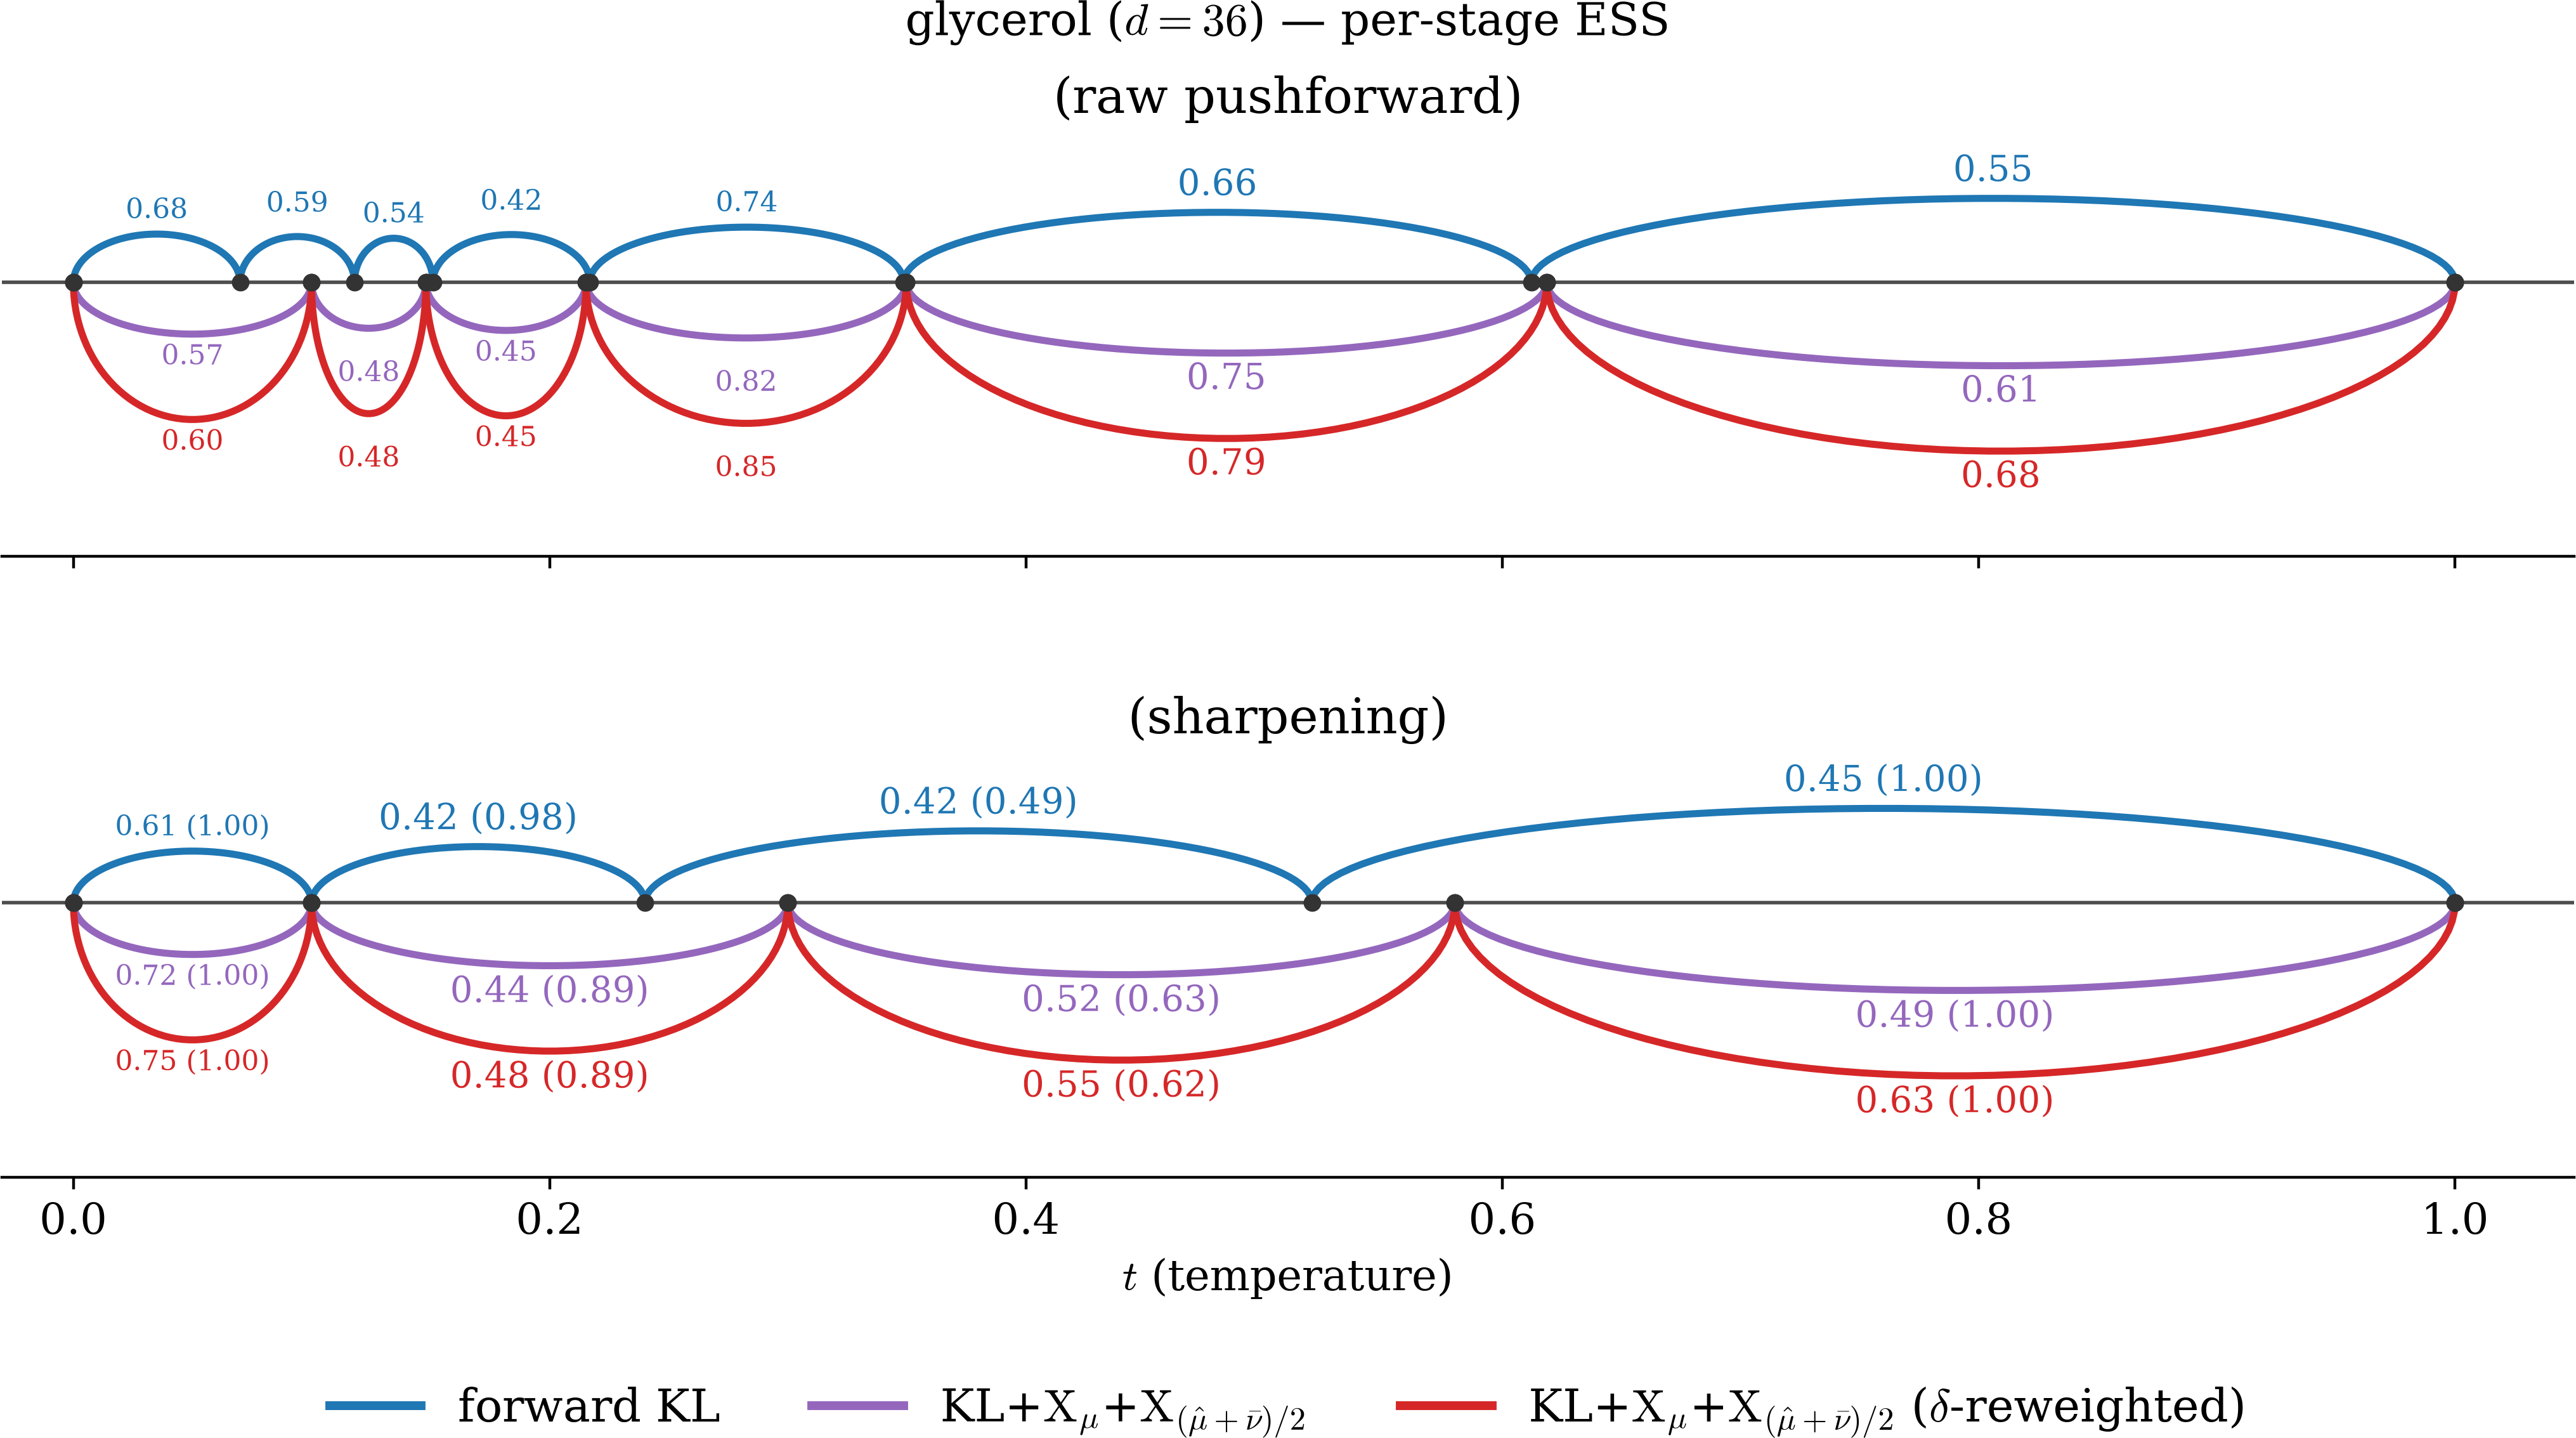
\includegraphics[width=\textwidth]{figures/Molecular_BG/glycerol_36d/ladder.png}
    \caption{Glycerol per-stage validation $\ESS$ as annealing-ladder arcs, raw (top) and sharpen (bottom).
    In each row forward KL is drawn above the axis (blue), $\KL{+}\X_\mu{+}\X_{(\hat\mu+\bar\nu)/2}$ below
    (purple), and its $\delta$-reweighted variant further below (red). Each arc is an accepted stage; the apex
    label is that stage's validation $\ESS$; a cross marks a bridge the ladder failed to reach.}
    \label{fig: glycerol-ladder}
\end{figure}

Glycerol is achiral (each torsion marginal is even, $p(\phi) = p(-\phi)$; Figure~\ref{fig: glycerol-dihedrals}), and every rotatable torsion is
three-fold: gauche$^{\pm}$ near $\pm 60^\circ$ and trans near $180^\circ$ (Figure~\ref{fig: glycerol-conformers}). The $\pm\phi$ symmetry pairs
gauche$^{-}\!\leftrightarrow$\,gauche$^{+}$ and leaves trans self-symmetric, so the joint target over the five
rotatable torsions is combinatorially multimodal (dozens of conformers), which is what the wide-coverage pool
must cover.

\begin{figure}[htbp]
    \centering
    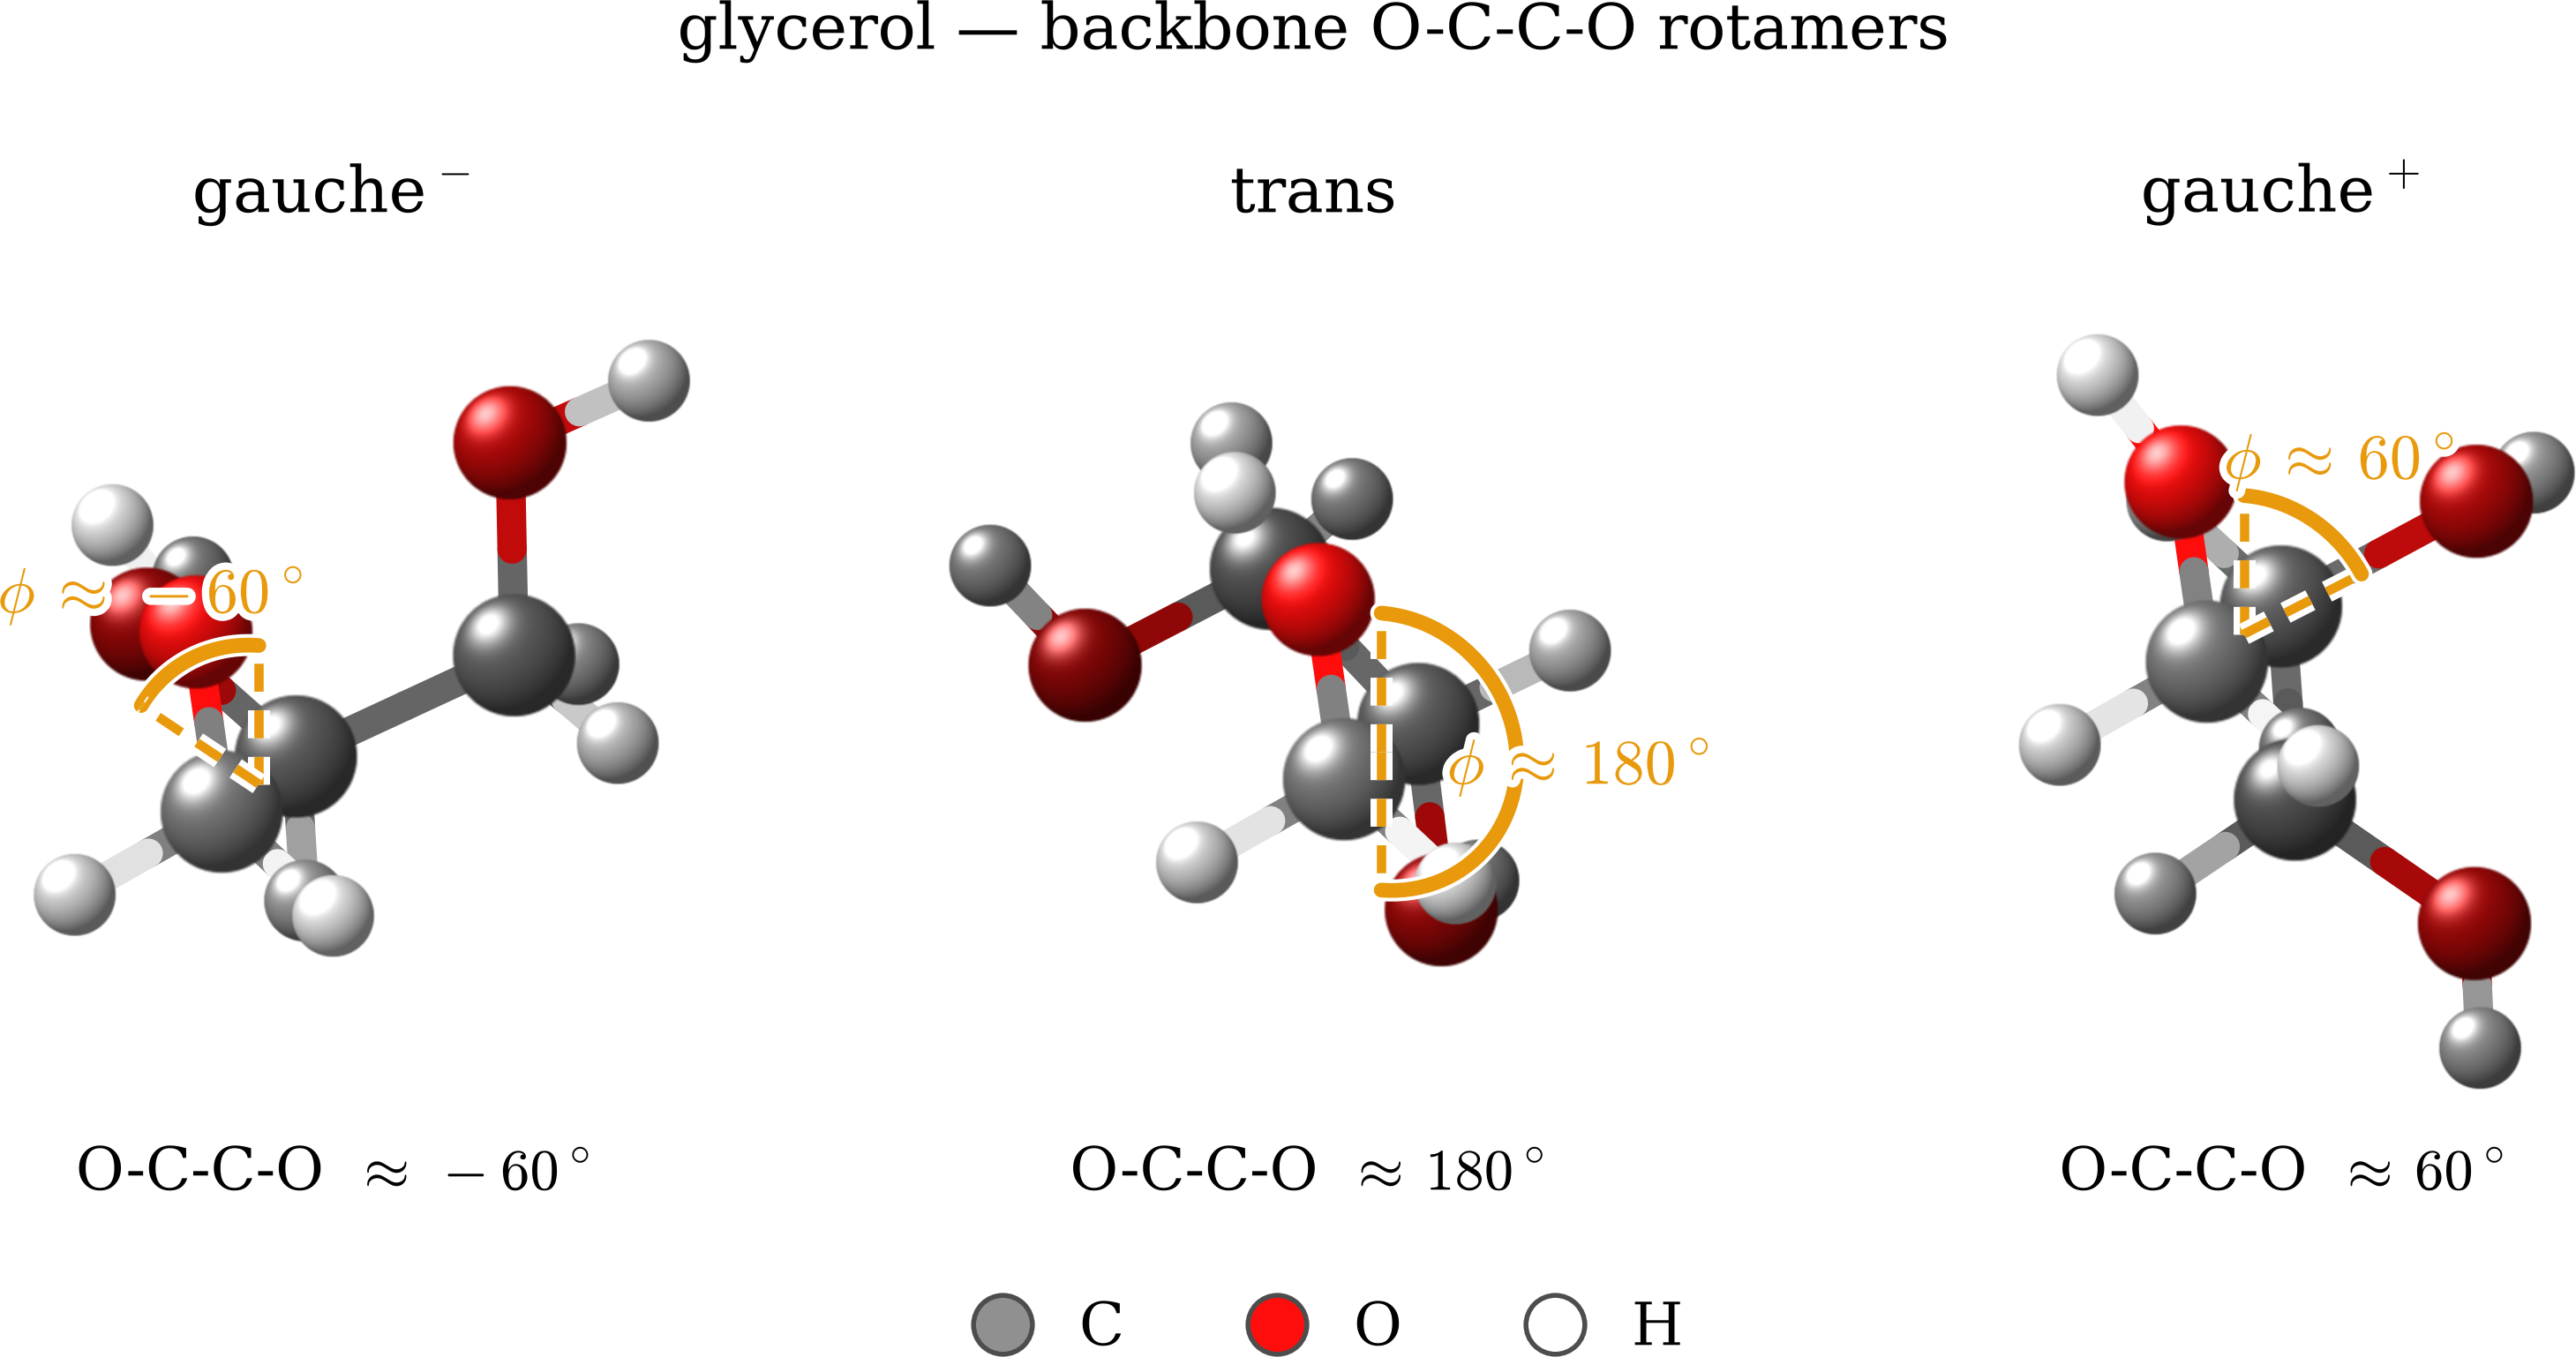
\includegraphics[width=0.8\textwidth]{figures/Molecular_BG/glycerol_36d/conformers.png}
    \caption{Typical glycerol configurations at the three states of the backbone O-C-C-O torsion:
    gauche$^-$ ($-60^\circ$), trans ($180^\circ$), gauche$^+$ ($+60^\circ$). The gold arc marks the dihedral
    $\phi$; ball-and-stick (C grey, O red, H white).}
    \label{fig: glycerol-conformers}
\end{figure}

\begin{figure}[htbp]
    \centering
    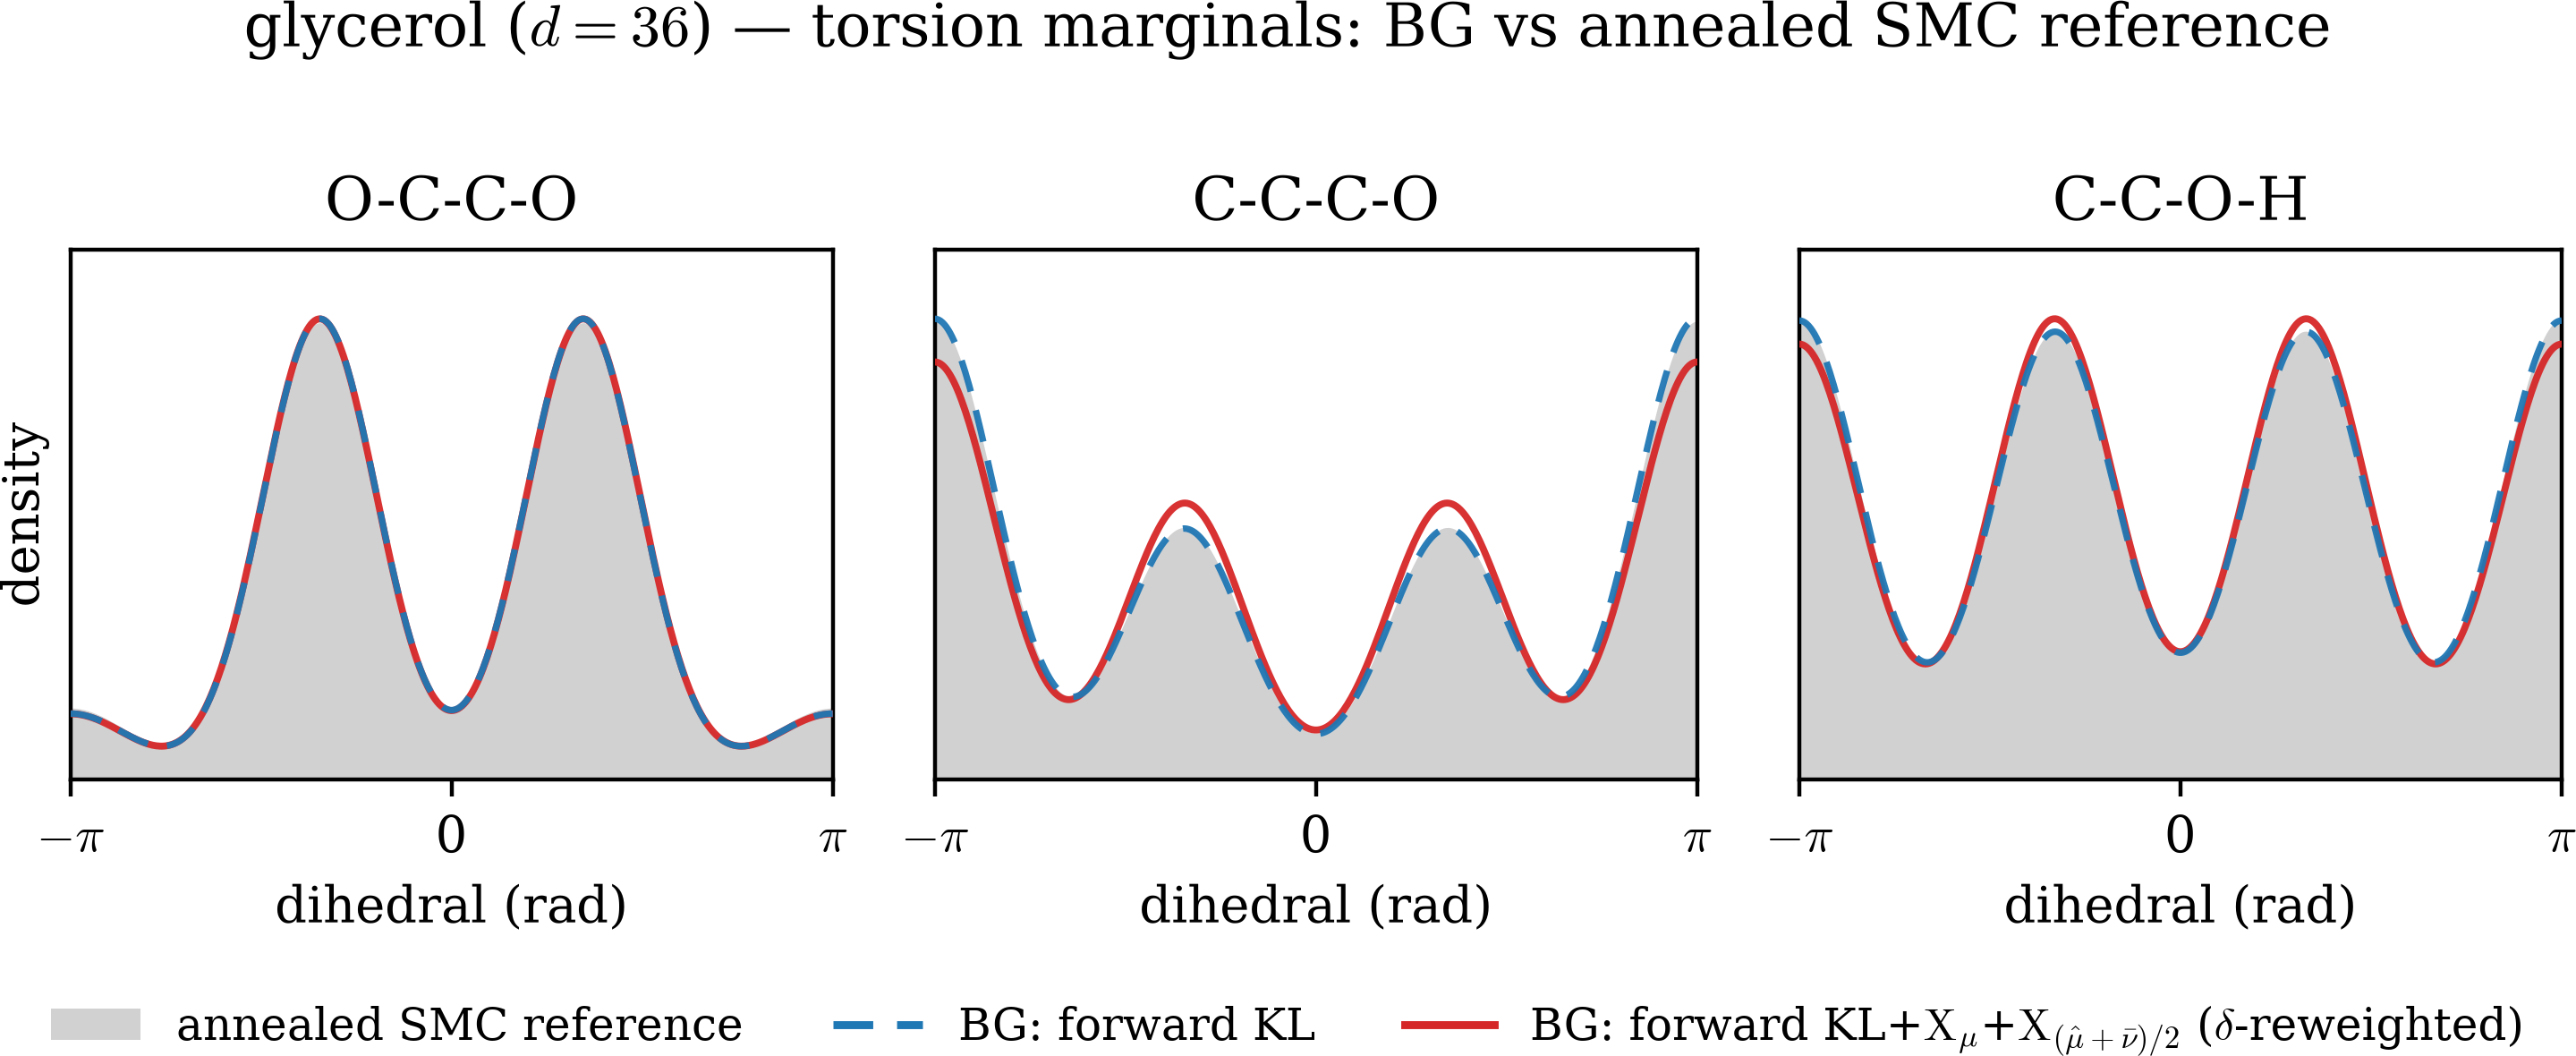
\includegraphics[width=0.8\textwidth]{figures/Molecular_BG/glycerol_36d/dihedrals.png}
    \caption{Glycerol torsion marginals of both generators against a converged annealed SMC reference
    (grey): forward KL (blue) and
    $\KL{+}\X_\mu{+}\X_{(\hat\mu+\bar\nu)/2}$, $\delta$-reweighted (red), both sharpened with the cap annealed
    to $e_{\mathrm{cap}} = 200$ kJ/mol. Both recover the multimodal gauche$^{\pm}$/trans structure of the characteristic glycerol
    torsions.}
    \label{fig: glycerol-dihedrals}
\end{figure}

\FloatBarrier
\subsubsection{Diethanolamine ($d = 48$)}
\label{sec: dea}

We test the generator on the full internal-coordinate diethanolamine target (\mbox{HN(CH$_2$CH$_2$OH)$_2$},
$d = 48$), comparing the two best losses under the same sharpening schedule (the soft cap geometrically
annealed $e_{\mathrm{cap}}\!:\!100\!\to\!200$ kJ/mol, a Monte Carlo sharpening step per stage): forward KL, and the X-regularized
$\KL{+}\X_\mu{+}\X_{(\hat\mu+\bar\nu)/2}$ with the $\delta$-reweighted quench and temper ($\delta = 0.1$).
Forward KL reaches $t = 1$ in $K = 6$ stages, the X-regularized loss in $K = 5$, a single direct
$0.65 \to 1$ step.

\begin{table}[h]
    \centering
    \small
    \begin{tabular}{@{}lccc@{}}
        \toprule
        loss & $K$ & wall (min) & $F$ \\
        \midrule
        annealed SMC                                            & 10 & 7 & 1455.44 \\
        forward KL                                              & 6 & 896 & 92.60 \\
        $\KL{+}\X_\mu{+}\X_{(\hat\mu+\bar\nu)/2}$, $\delta$-rw. & 5 & 782 & \textbf{35.90} \\
        \bottomrule
    \end{tabular}
    \caption{Diethanolamine ($d = 48$): two trained-flow losses and an annealed SMC reference, all with
    a per-stage Monte Carlo sharpening reweight (cap $e_{\mathrm{cap}}$ geometrically annealed $100 \to 200$ kJ/mol): ladder length
    $K$, training wall-clock, and the error-propagation factor $F$ \eqref{eq: F} (smaller better; $F$ includes
    the sharpening reweight). $\delta$-rw.\ $=$
    $\delta$-reweighted quench and temper.}
    \label{tab: dea}
\end{table}

The X-regularized loss with $\delta$-reweighting reaches $F = 35.9$ versus forward KL's $F = 92.6$ (Table~\ref{tab: dea}), a
${\sim}2.6\times$ reduction in importance-weight waste at identical settings (glycerol showed a comparable
${\sim}3.1\times$ gap, $14.2$ vs $44.0$). The advantage shows in the late, sharp stages and in the ladder
length: forward KL's per-stage validation $\ESS$ stalls at $0.46$--$0.53$ and it needs $6$ rungs to reach
$t = 1$, whereas the $\KL{+}\X_\mu{+}\X_{(\hat\mu+\bar\nu)/2}$, $\delta$-reweighted run holds a higher $\ESS$
($0.74$ on the final, direct $0.65 \to 1$ step) and reaches $t = 1$ in $5$ (Figure~\ref{fig: dea-ladder}). This
is a singular, high-dimensional, combinatorially multimodal target, so each run is a multi-hour computation;
closing it efficiently is the practical contribution of the X-regularized loss.

\begin{figure}[htbp]
    \centering
    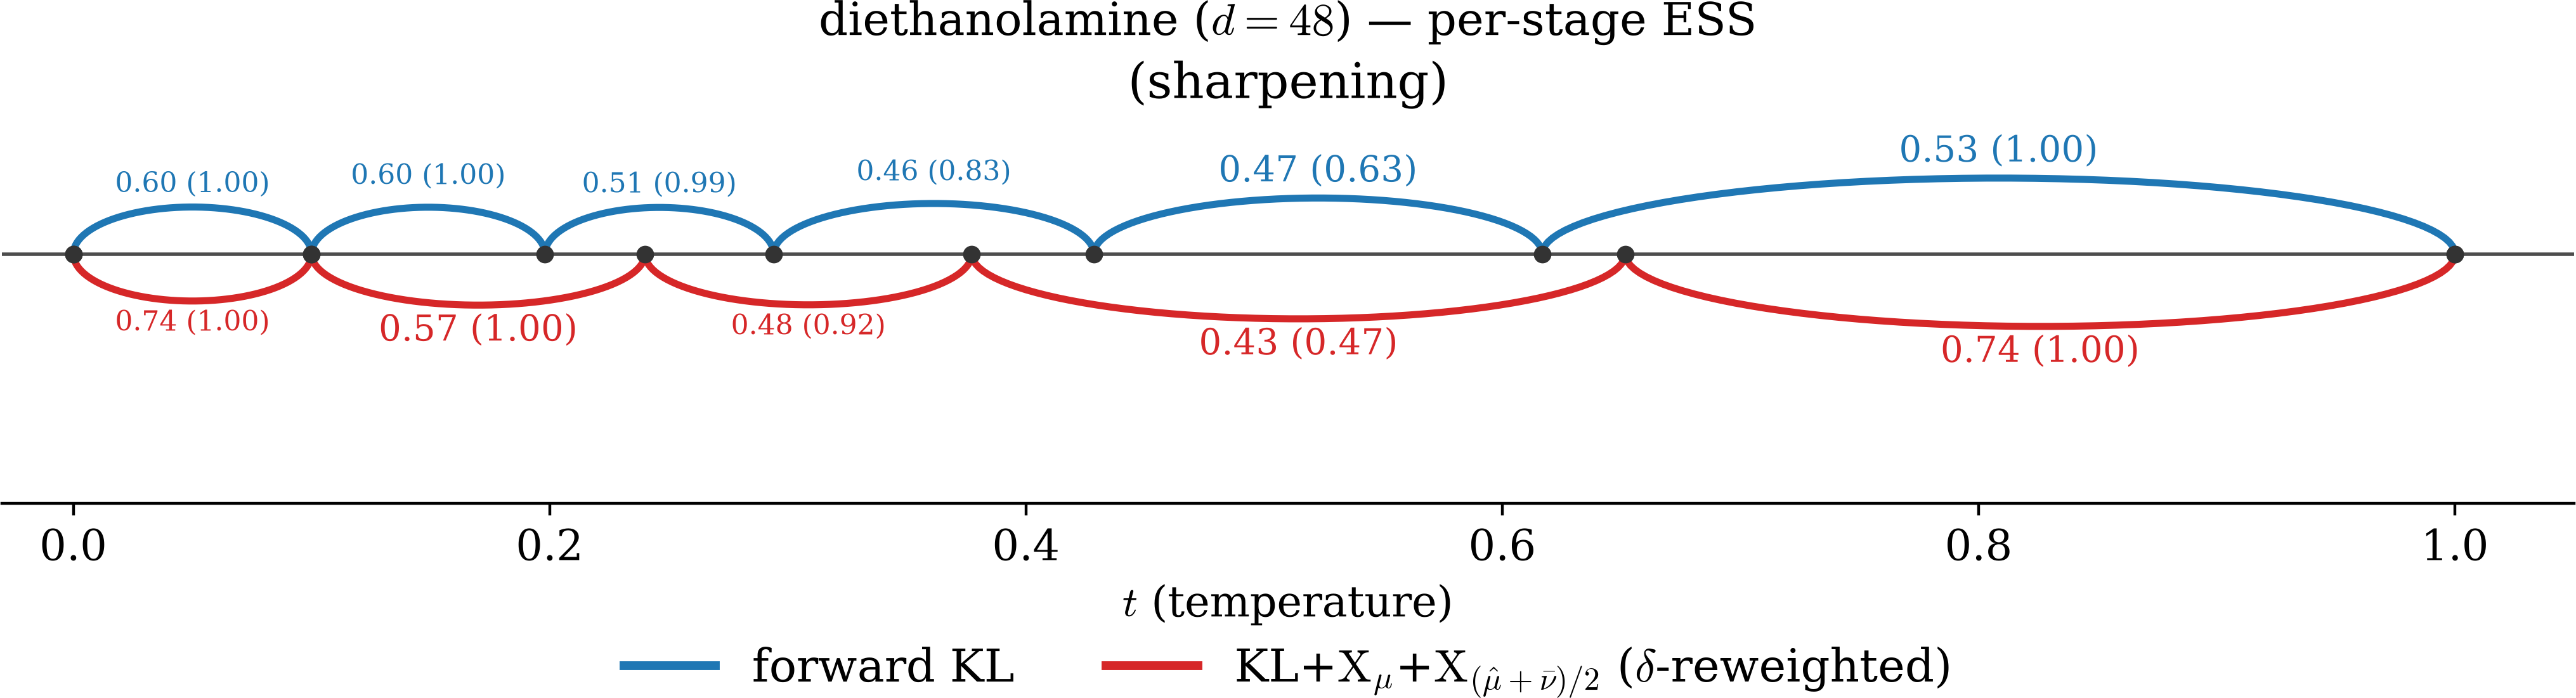
\includegraphics[width=\textwidth]{figures/Molecular_BG/diethanolamine_48d/ladder.png}
    \caption{Diethanolamine per-stage $\ESS$ as annealing-ladder arcs (sharpening schedule): forward KL above
    the axis (blue), $\KL{+}\X_\mu{+}\X_{(\hat\mu+\bar\nu)/2}$, $\delta$-reweighted, below (red). Each arc is an
    accepted stage; the apex label is that stage's validation $\ESS$, with the sharpening $\ESS$ in
    parentheses.}
    \label{fig: dea-ladder}
\end{figure}

Diethanolamine has a plane of symmetry (each torsion marginal is even, $p(\phi) = p(-\phi)$); its rotatable
backbone torsions, O-C-C-N and C-C-N-C along the ethanolamine arms plus the hydroxyl rotations,
are each multi-well (gauche$^{\pm}$/trans, Figure~\ref{fig: dea-conformers}), so the joint target is combinatorially multimodal, which the
wide-coverage pool must cover.

\begin{figure}[htbp]
    \centering
    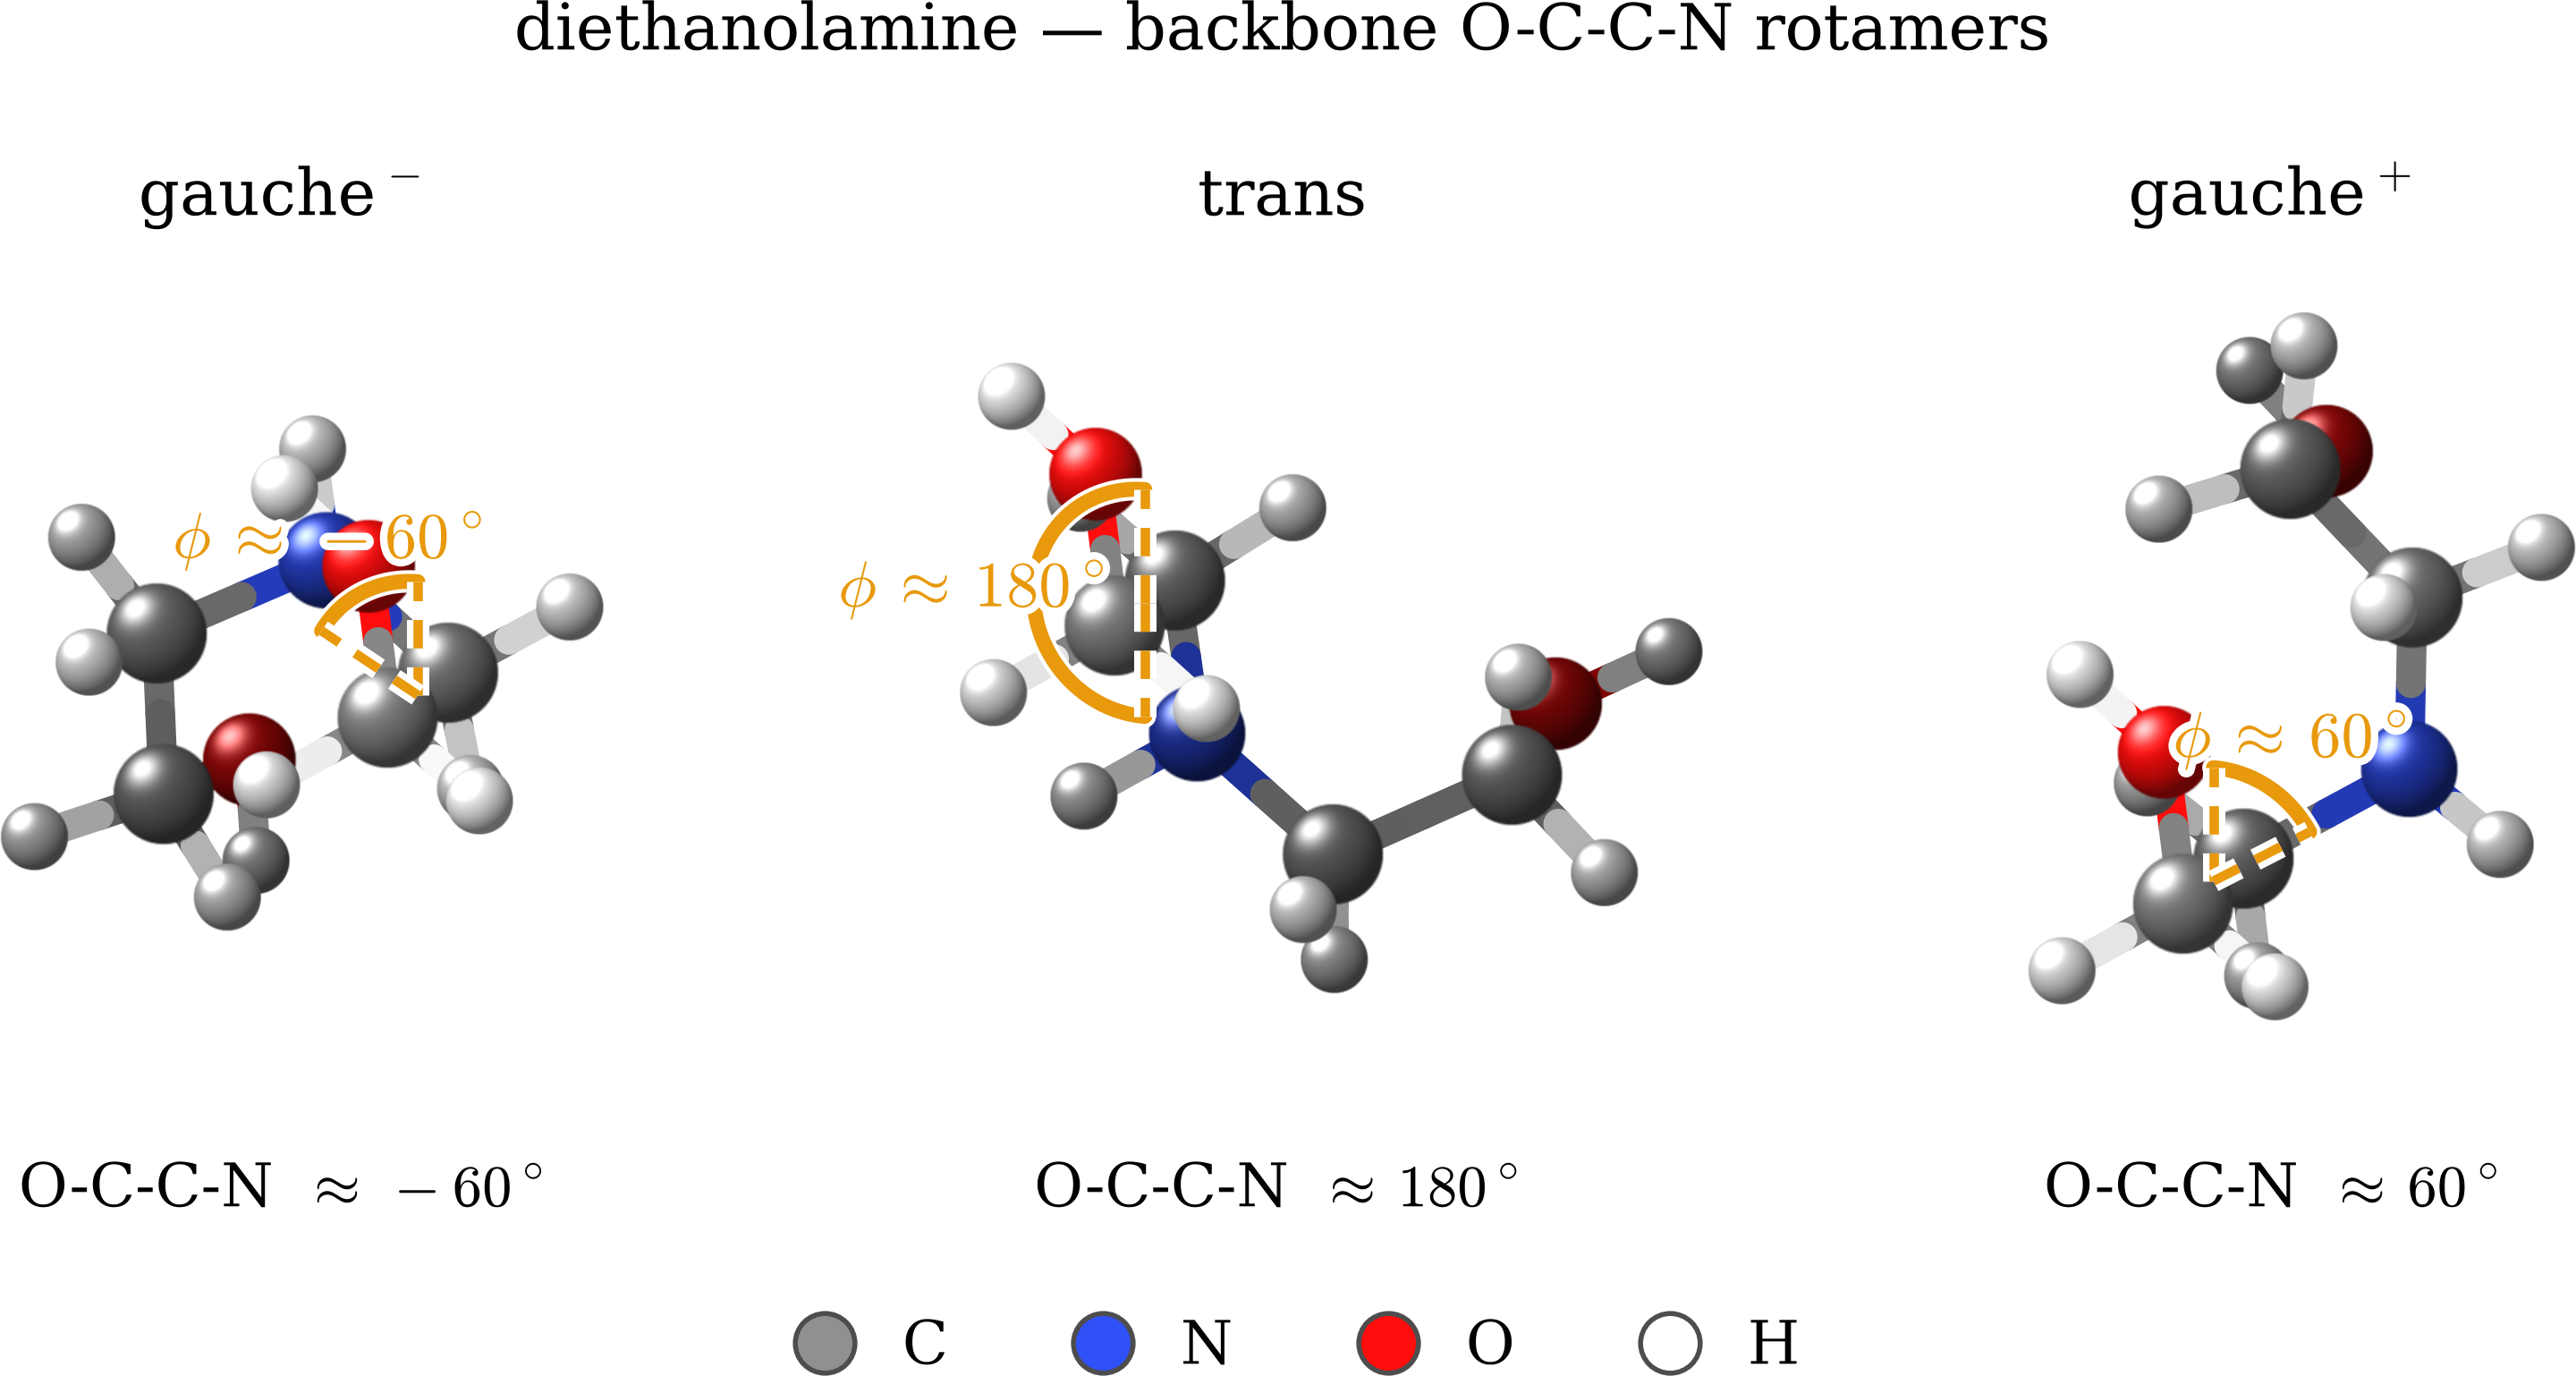
\includegraphics[width=0.8\textwidth]{figures/Molecular_BG/diethanolamine_48d/conformers.png}
    \caption{Typical diethanolamine configurations at the three states of a backbone O-C-C-N torsion:
    gauche$^-$ ($-60^\circ$), trans ($180^\circ$), gauche$^+$ ($+60^\circ$). The gold arc marks the dihedral
    $\phi$; ball-and-stick (C grey, N blue, O red, H white).}
    \label{fig: dea-conformers}
\end{figure}

\begin{figure}[htbp]
    \centering
    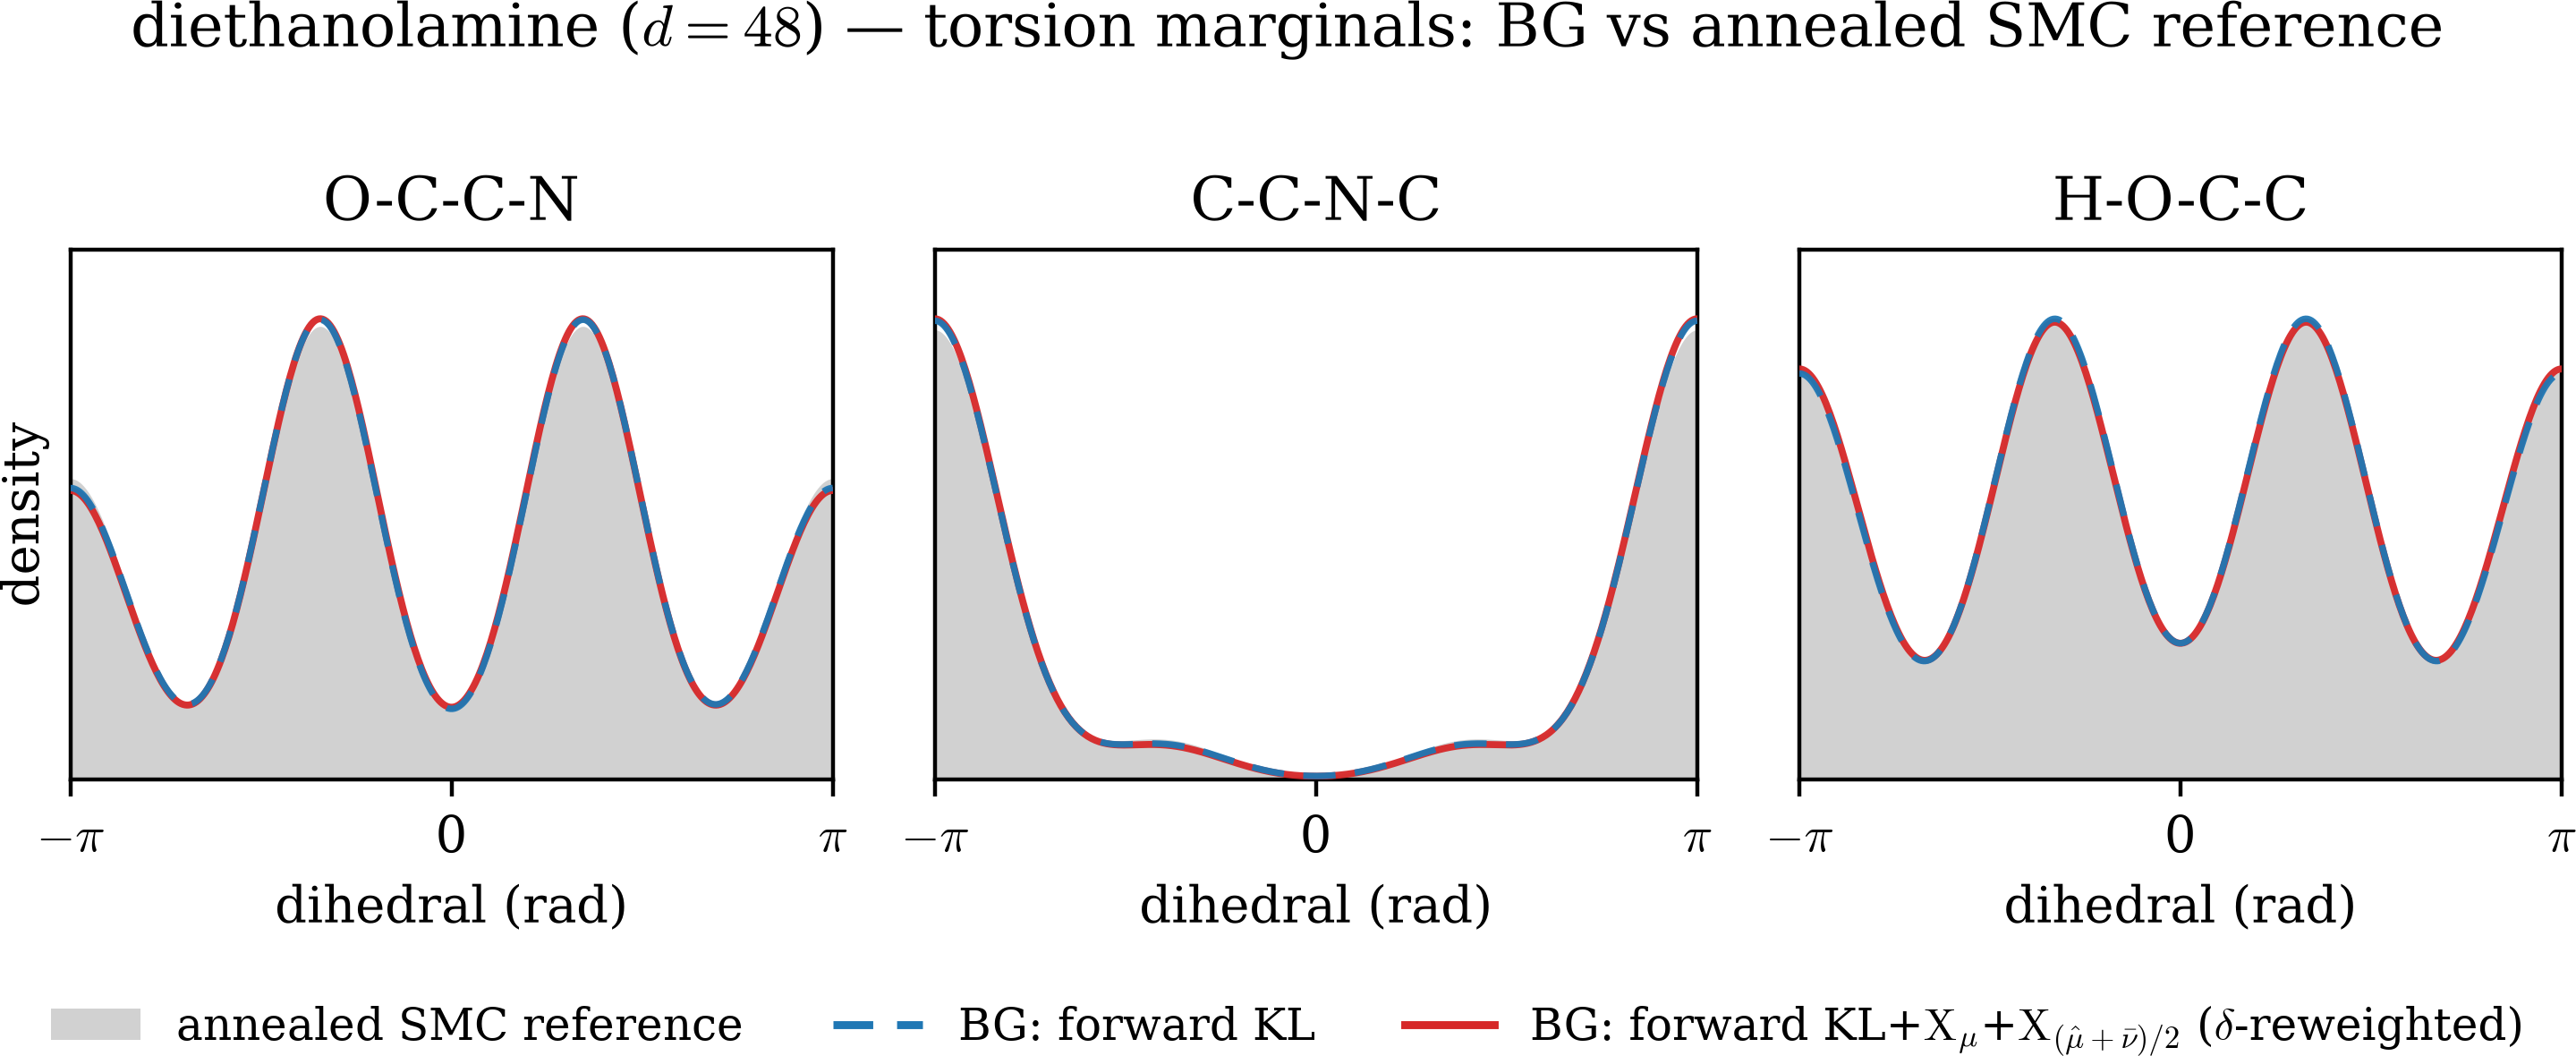
\includegraphics[width=0.8\textwidth]{figures/Molecular_BG/diethanolamine_48d/dihedrals.png}
    \caption{Diethanolamine torsion marginals of both generators against a converged annealed SMC
    reference (grey): forward KL (blue) and
    $\KL{+}\X_\mu{+}\X_{(\hat\mu+\bar\nu)/2}$, $\delta$-reweighted (red), both sharpened with the cap annealed
    to $e_{\mathrm{cap}} = 200$ kJ/mol. Both recover the multimodal backbone torsions and track the annealed SMC reference.}
    \label{fig: dea-dihedrals}
\end{figure}

Against the annealed SMC reference (Figure~\ref{fig: dea-dihedrals}) the two losses are visually indistinguishable: both
recover the multimodal backbone torsions and neither is discernibly closer to the reference. The separation is in
efficiency, not in the sampled marginals: $\KL{+}\X_\mu{+}\X_{(\hat\mu+\bar\nu)/2}$ reaches $t = 1$ in fewer
stages ($5$ vs $6$) with a higher final-step $\ESS$ ($0.74$ vs $0.53$), a $\sim 2.6\times$ smaller
error-propagation factor ($F = 35.9$ vs $92.6$), and fewer rejected stage attempts in the early ladder
(stages 2--4: $1,1,0$ rejections versus forward KL's $2,2,1$). Switching the trained flow off entirely (the
identity map at every stage, i.e.\ plain adaptive annealed SMC over the same ladder) gives $F = 1455$ in
$K = 10$ stages. The trained
X-regularized flow therefore cuts the propagation factor by ${\sim}40\times$ and halves the ladder length
($5$ vs $10$): on this singular target the transport map adds even more over annealing alone than on glycerol,
a justification for training a flow.

\FloatBarrier
\subsubsection{Alanine dipeptide ($d = 60$)}
\label{sec: adp}

We push the generator to alanine dipeptide (Ac-Ala-NHMe), the canonical Boltzmann generator benchmark,
in full internal coordinates ($d = 60$). The qualitative step up from glycerol and diethanolamine is the
target's character: those are dominated by smooth rotatable-bond multimodality, whereas alanine dipeptide folds the backbone
tightly enough that the Lennard-Jones clash core, not the torsion profile, sets the hardest part of the
anneal. We report the X-regularized loss only ($\KL{+}\X_\mu{+}\X_{(\hat\mu+\bar\nu)/2}$,
$\delta$-reweighted, $\delta = 0.1$), with a per-stage Monte Carlo sharpening in which \emph{both} the cap
$e_{\mathrm{cap}}\!:\!100\!\to\!200$ kJ/mol and the clash floor $r_{\mathrm{floor}}\!:\!0.2\!\to\!0.1$ nm are annealed arithmetically, unlike the geometric
$e_{\mathrm{cap}}$ schedule of glycerol and diethanolamine; alanine dipeptide is also the only target that anneals $r_{\mathrm{floor}}$, which glycerol and diethanolamine hold fixed at $0.1$ nm. The run reaches $t = 1$ in $K = 11$ stages at $F^{*} = 67.95$,
with every stage holding validation $\ESS \Ge 0.51$ and sharpening $\ESS \Ge 0.95$
(Table~\ref{tab: adp}, Figure~\ref{fig: adp-ess}). The bare composed flow's end-to-end $\ESS$ against the sharp
target, from a single importance reweight of source samples pushed through the fully composed $K$-stage map and
scored against $U_{1,1}$, is only ${\sim}5\times10^{-6}$, so the per-stage sharpening, not a raw pushforward,
is the deliverable.

\begin{table}[h]
    \centering
    \small
    \begin{tabular}{@{}lccc@{}}
        \toprule
        loss & $K$ & wall (min) & $F^{*}$ \\
        \midrule
        annealed SMC                                           & 12 & 23  & 129.70$^{*}$ \\
        $\KL{+}\X_\mu{+}\X_{(\hat\mu+\bar\nu)/2}$, $\delta$-rw. & 11 & ${\sim}1000$ & \textbf{67.95}$^{*}$ \\
        \bottomrule
    \end{tabular}
    \caption{Alanine dipeptide ($d = 60$), the X-regularized loss with a per-stage Monte Carlo sharpening
    reweight (the cap $e_{\mathrm{cap}}$ and floor $r_{\mathrm{floor}}$ annealed arithmetically): ladder length $K$,
    wall-clock, and the error-propagation factor $F^{*}$ \eqref{eq: Fstar}, starred throughout because every
    entry uses the smooth validation $\ESS$ (smaller better; $F^{*}$ includes the sharpening reweight). The
    first row is an annealed SMC reference, the identity map over the same ladder.
    $\delta$-rw.\ $=$ $\delta$-reweighted quench and temper.}
    \label{tab: adp}
\end{table}

For comparison, the lighter targets close at $F = 14.2$ (glycerol) and $F = 35.9$ (diethanolamine) with the
same loss; alanine dipeptide's larger $F^{*}$ is the price of its singular nonbonded core, not of its multimodality. Three
alanine-dipeptide-only factors nonetheless make this $F^{*}$ read smaller than a strict like-for-like extension of that trend:
the per-stage $\ESS$ is the smooth estimator $\ESS^{\mathrm{val}*}_k$ \eqref{eq: smooth-ess} rather than the raw weighted
$\ESS$; $r_{\mathrm{floor}}$ is annealed alongside the cap; and the ladder is much longer ($K = 11$
versus $4$ and $5$), its smaller per-step jumps keeping each per-stage $\ESS$ high. All three raise the
per-stage $\ESS$ entering $F^{*}$, and none applied to the lighter targets.

\begin{figure}[htbp]
    \centering
    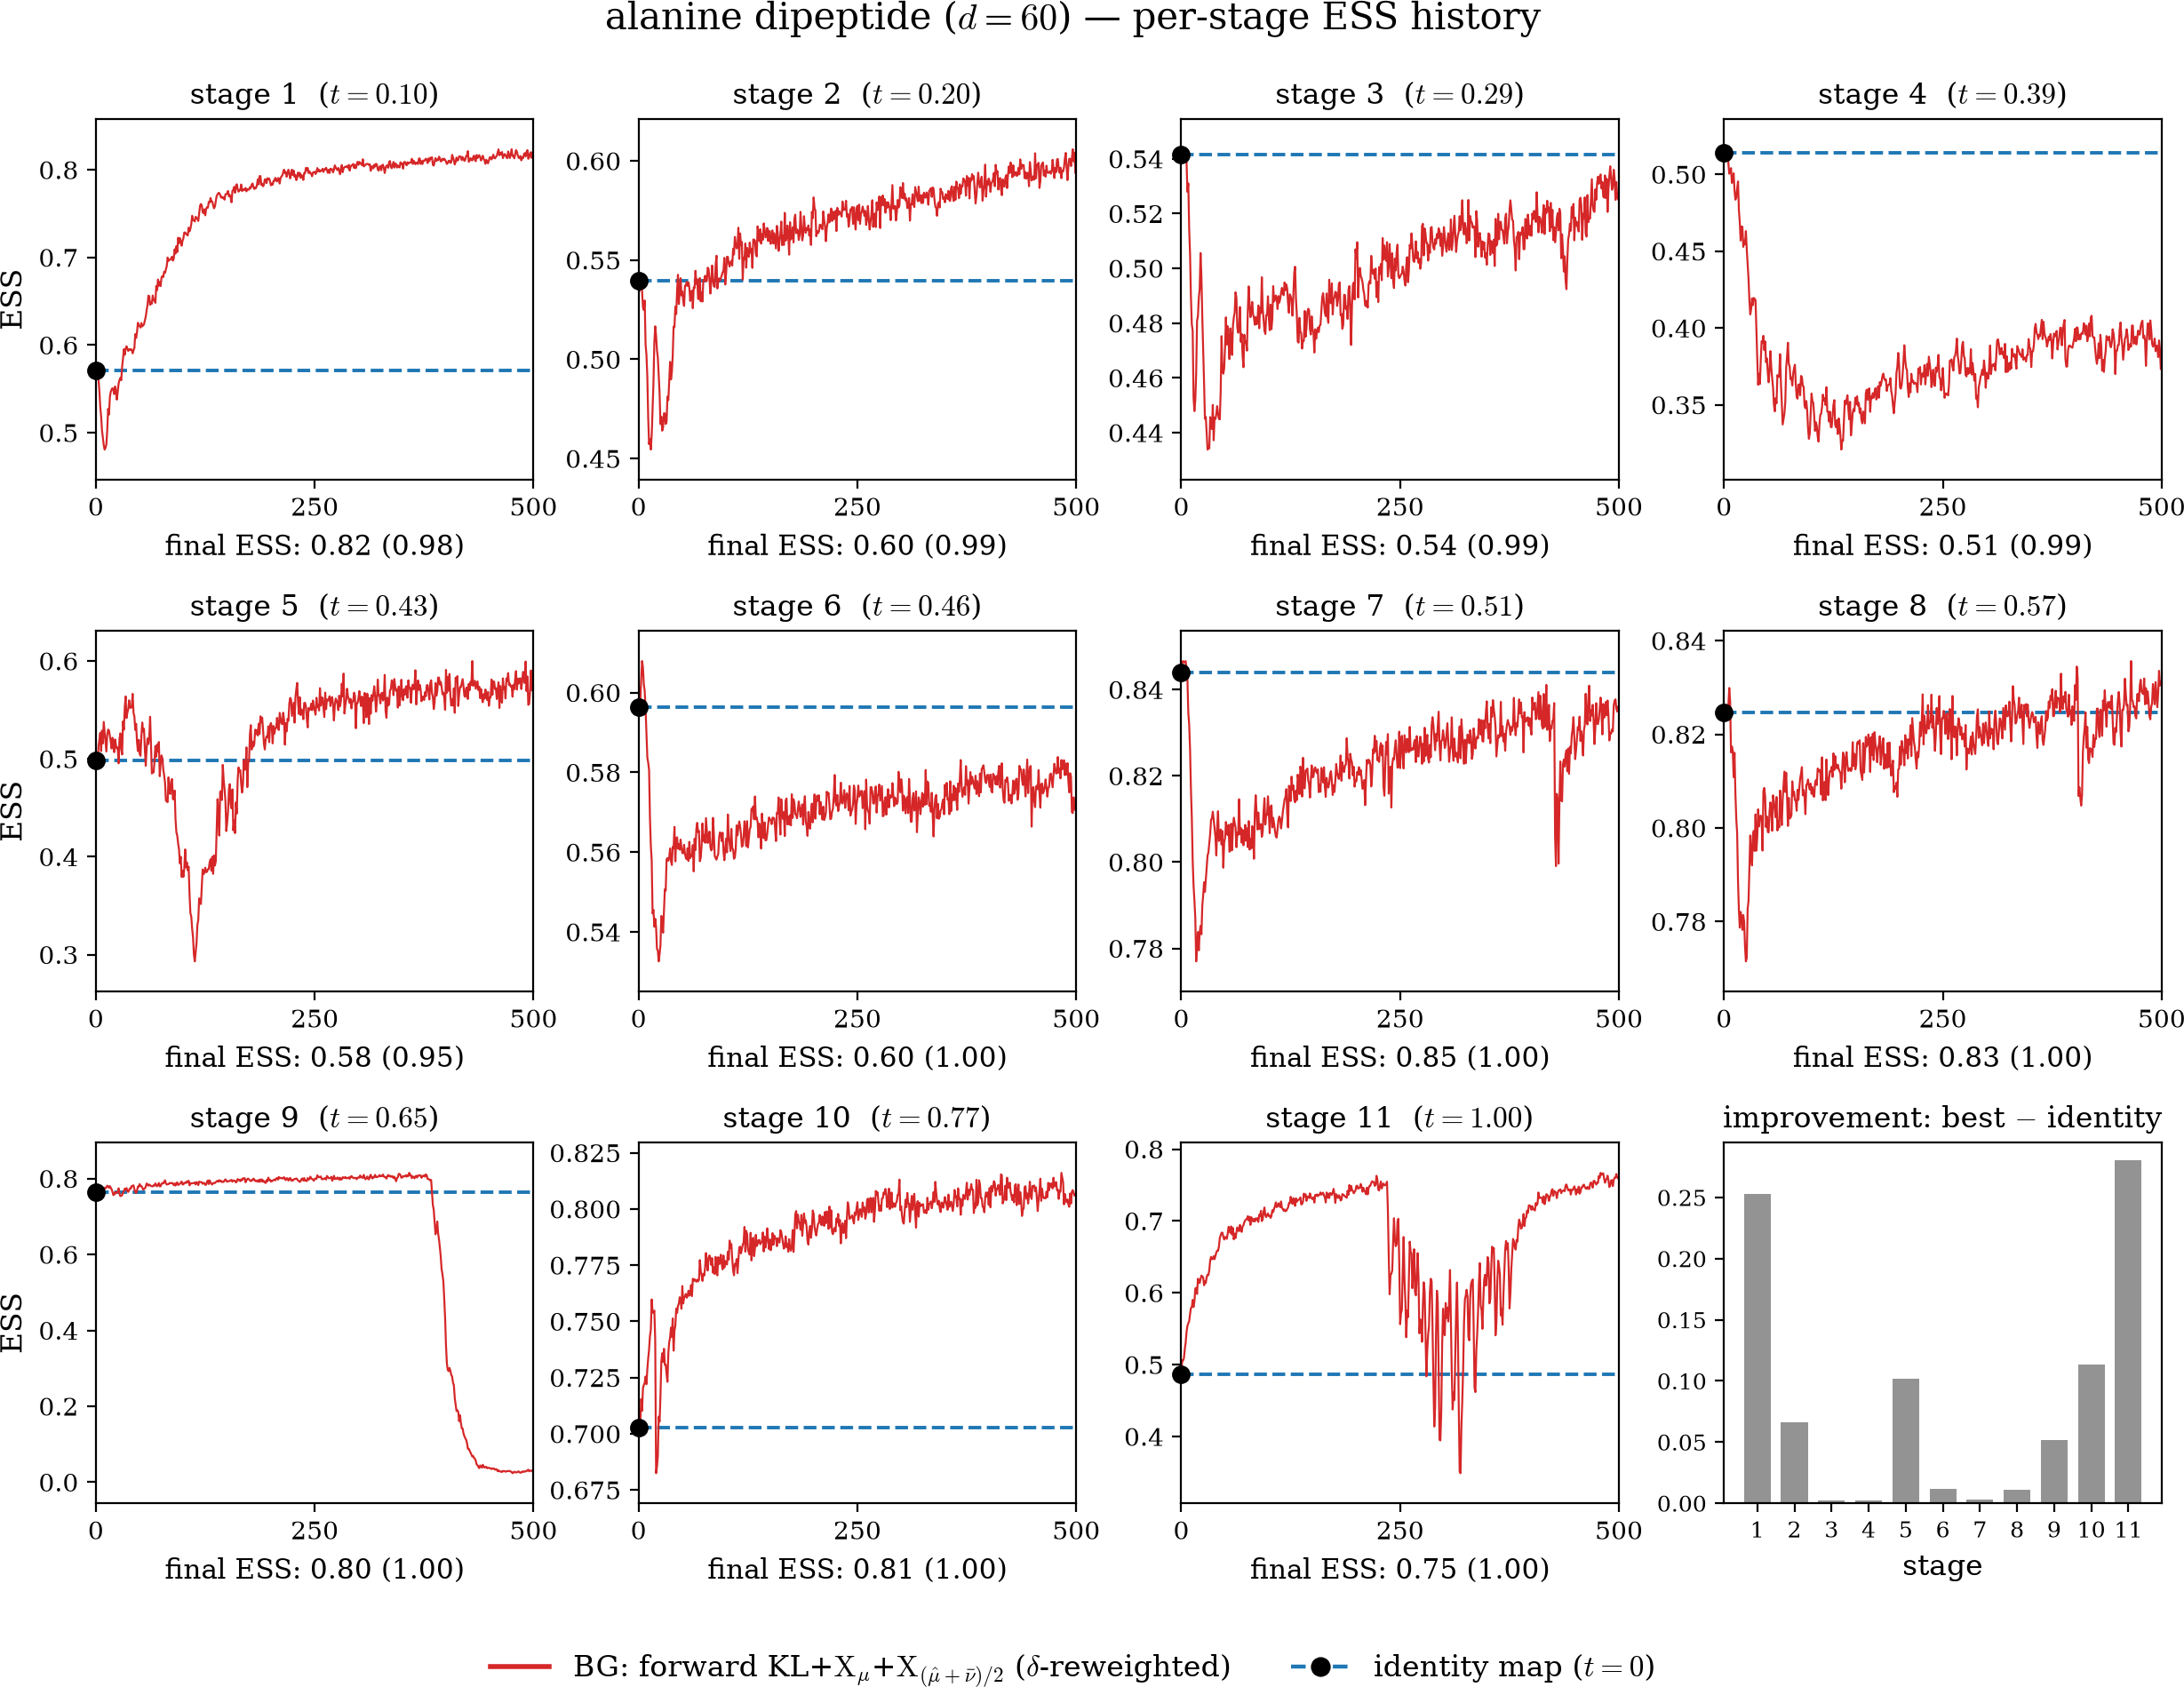
\includegraphics[width=\textwidth]{figures/Molecular_BG/adp_60d/ess_history.png}
    \caption{Alanine dipeptide per-stage $\ESS$ history: each panel is the per-step effective sample size
    during that stage's X-regularized $\delta$-reweighted flow training (red), against the identity-map
    baseline at $t = 0$ (blue dashed). Below each panel is that stage's accepted validation $\ESS$ with the
    sharpening $\ESS$ in parentheses. The dip across $t \approx 0.29$--$0.43$ is the clash bottleneck, with
    $\ESS$ recovering to $\approx 0.8$ once the cap is sharp enough to separate the basins.}
    \label{fig: adp-ess}
\end{figure}

The instability is sharply localized to a clash bottleneck near $t \approx 0.3$--$0.43$. The stages spanning
$t \approx 0.29$--$0.43$ (soft cap $e_{\mathrm{cap}} \approx 129$--$143$ kJ/mol) are where the nonbonded core first bites: the run
minimum validation $\ESS$ ($0.51$ at $t = 0.39$) sits here, and these are the \emph{only} stages that shrink
the step (shrunk once at stages $3,4,5$) or retry heavily (3 attempts at stages $5,6$). Below
$t \approx 0.3$ the torsions still dominate and the flow trains in a single attempt; above $t \approx 0.5$ the
cap is sharp enough that the basins separate cleanly and $\ESS$ recovers to ${\approx}0.8$. The binding
constraint for alanine dipeptide is the clash singularity, not the multimodality: the qualitative difference from the
$d \Le 48$ molecules, and the reason the three devices of Section~\ref{sec: mol-engineering} (particle drop,
best $\ESS$ gate snapshots, $r$-floor anneal), inert on glycerol and diethanolamine, were necessary here.

The per-stage $\ESS$ history (Figure~\ref{fig: adp-ess}) exposes two coupled instabilities that the best $\ESS$
gate works around but does not cure. First, the within-stage $\ESS$ is \emph{non-monotone and unstable}: it
can rise, plateau, then drop abruptly (the sharp collapse late in the $t = 0.65$ stage and the volatility at
$t = 1$ are the clearest cases), so the last training step is frequently far below the best (stage~9's
training $\ESS$ decays to $0.03$ by step $500$ while the best $\ESS$ gate keeps a snapshot at validation
$\ESS = 0.80$). Second, near the clash bottleneck ($t \approx 0.3$--$0.5$) several flows \emph{degenerate
toward the identity map}: the best achievable $\ESS$ barely exceeds the $t = 0$ identity baseline
($\Delta = \text{best} - \text{identity} \approx 0$ at stages $3, 4, 7$), i.e.\ training fails to improve on
doing nothing. Both are understood consequences of the \emph{singularity of the potential}: the Lennard-Jones
$r \to 0$ divergence leaves the soft-capped target ill-conditioned exactly where the nonbonded core first
bites, so the gradient signal that would pull the flow off identity is weakest there. We report this as a
known limitation; robust remedies (stronger or adaptive regularization annealing, parameterizations tailored
to the repulsive wall) are left to future work.

\begin{figure}[htbp]
    \centering
    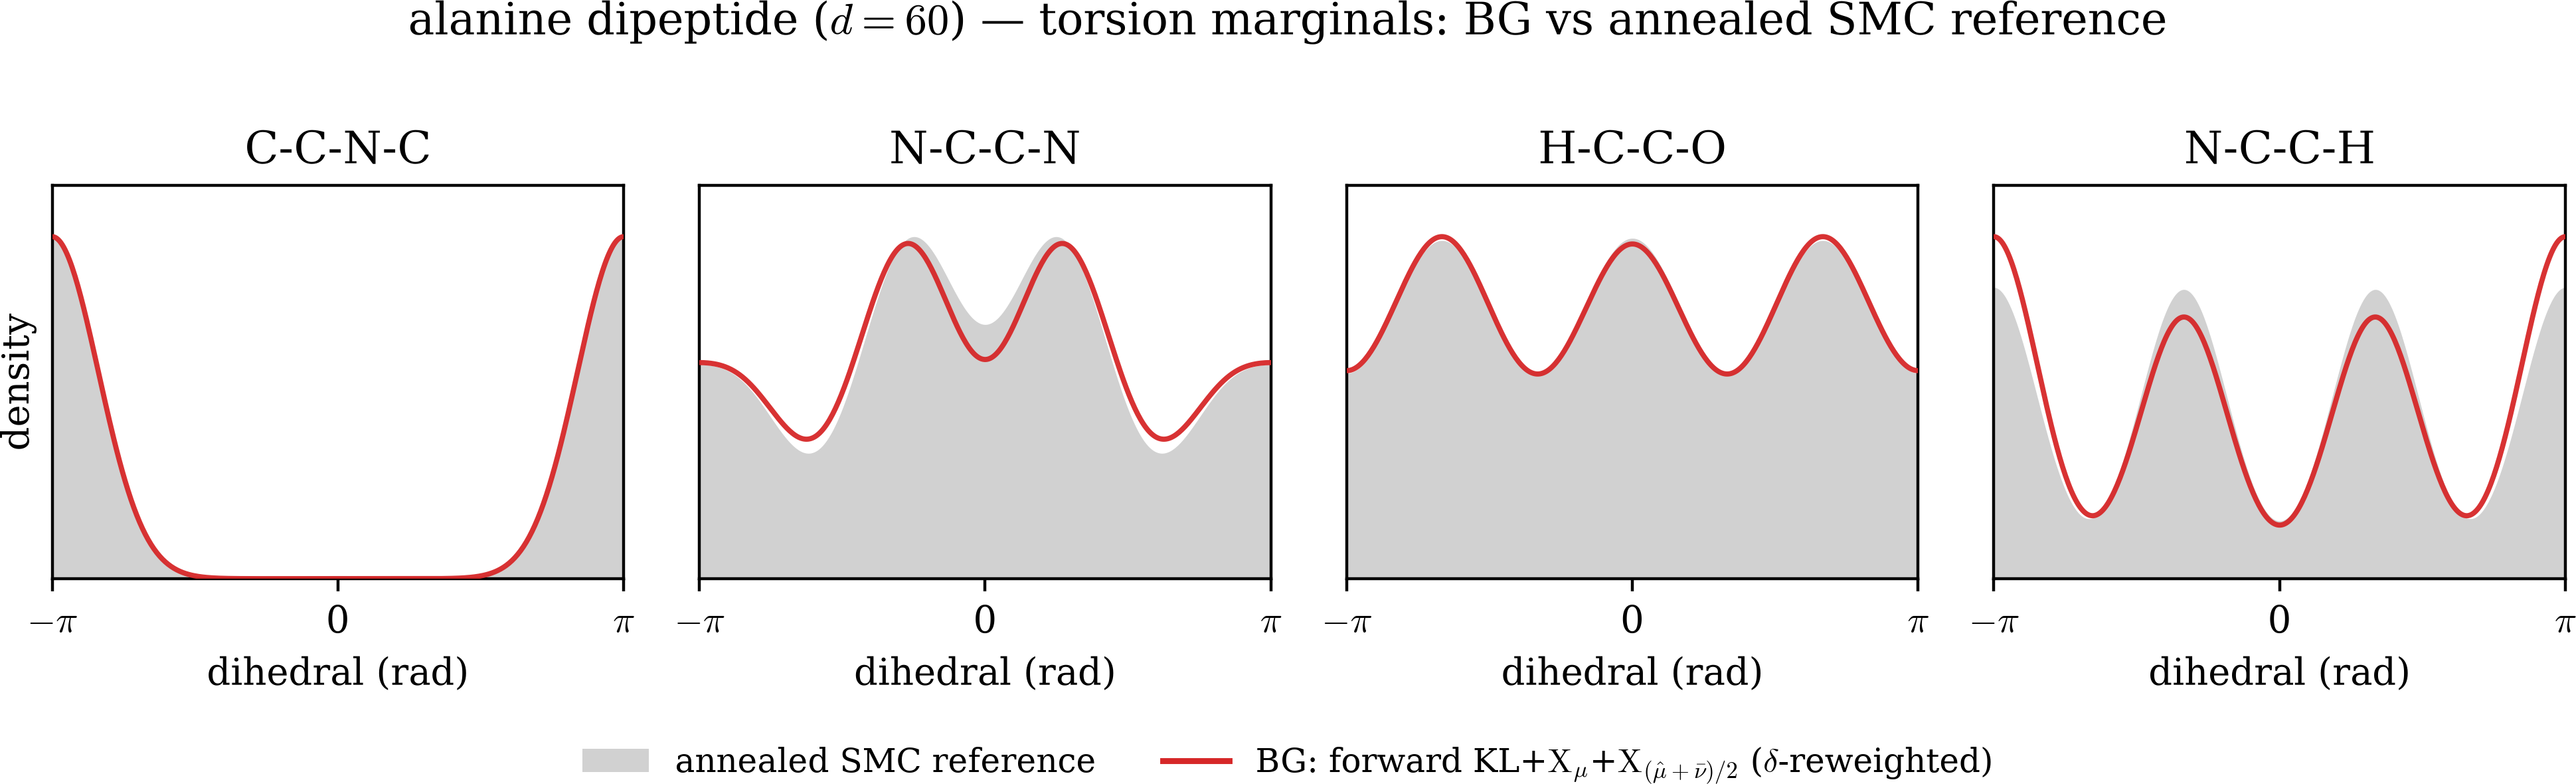
\includegraphics[width=\textwidth]{figures/Molecular_BG/adp_60d/dihedrals.png}
    \caption{Alanine dipeptide torsion marginals of the BG deliverable (red) against a converged
    annealed SMC reference (grey). The four most multimodal proper
    torsions are shown; the densities are $\pm\phi$-symmetrised, the achiral target having $p(\phi) = p(-\phi)$.
    The BG recovers the multimodal backbone torsions and tracks the reference; the peptide-bond torsion $\omega$ (C-C-N-C) is
    trans-dominant in the generator, the one torsion whose high rotation barrier also makes the uniform-init annealed SMC
    reference slow to converge.}
    \label{fig: adp-dihedrals}
\end{figure}

alanine dipeptide's backbone $\phi,\psi$ are multi-basin (Figure~\ref{fig: adp-dihedrals}), and a second, alanine-dipeptide-specific feature
is chirality: the classical force field is mirror-symmetric (every term in \eqref{eq: amber} is invariant
under reflection), so the L- and D-forms are isoenergetic. A physical MD trajectory stays in one form, as
inverting the $\mathrm{C}_\alpha$ needs bond breaking, but the internal-coordinate flow carries no chirality
constraint and emits \emph{both} (Figure~\ref{fig: adp-conformers}). In the Ramachandran
(Figure~\ref{fig: adp-rama}) this appears as the $(\phi,\psi)\!\to\!(-\phi,-\psi)$ point symmetry: the D-basins
are the exact mirror of the L-basins, each populated, where a single kinetically trapped physical trajectory
would show only one.

\begin{figure}[htbp]
    \centering
    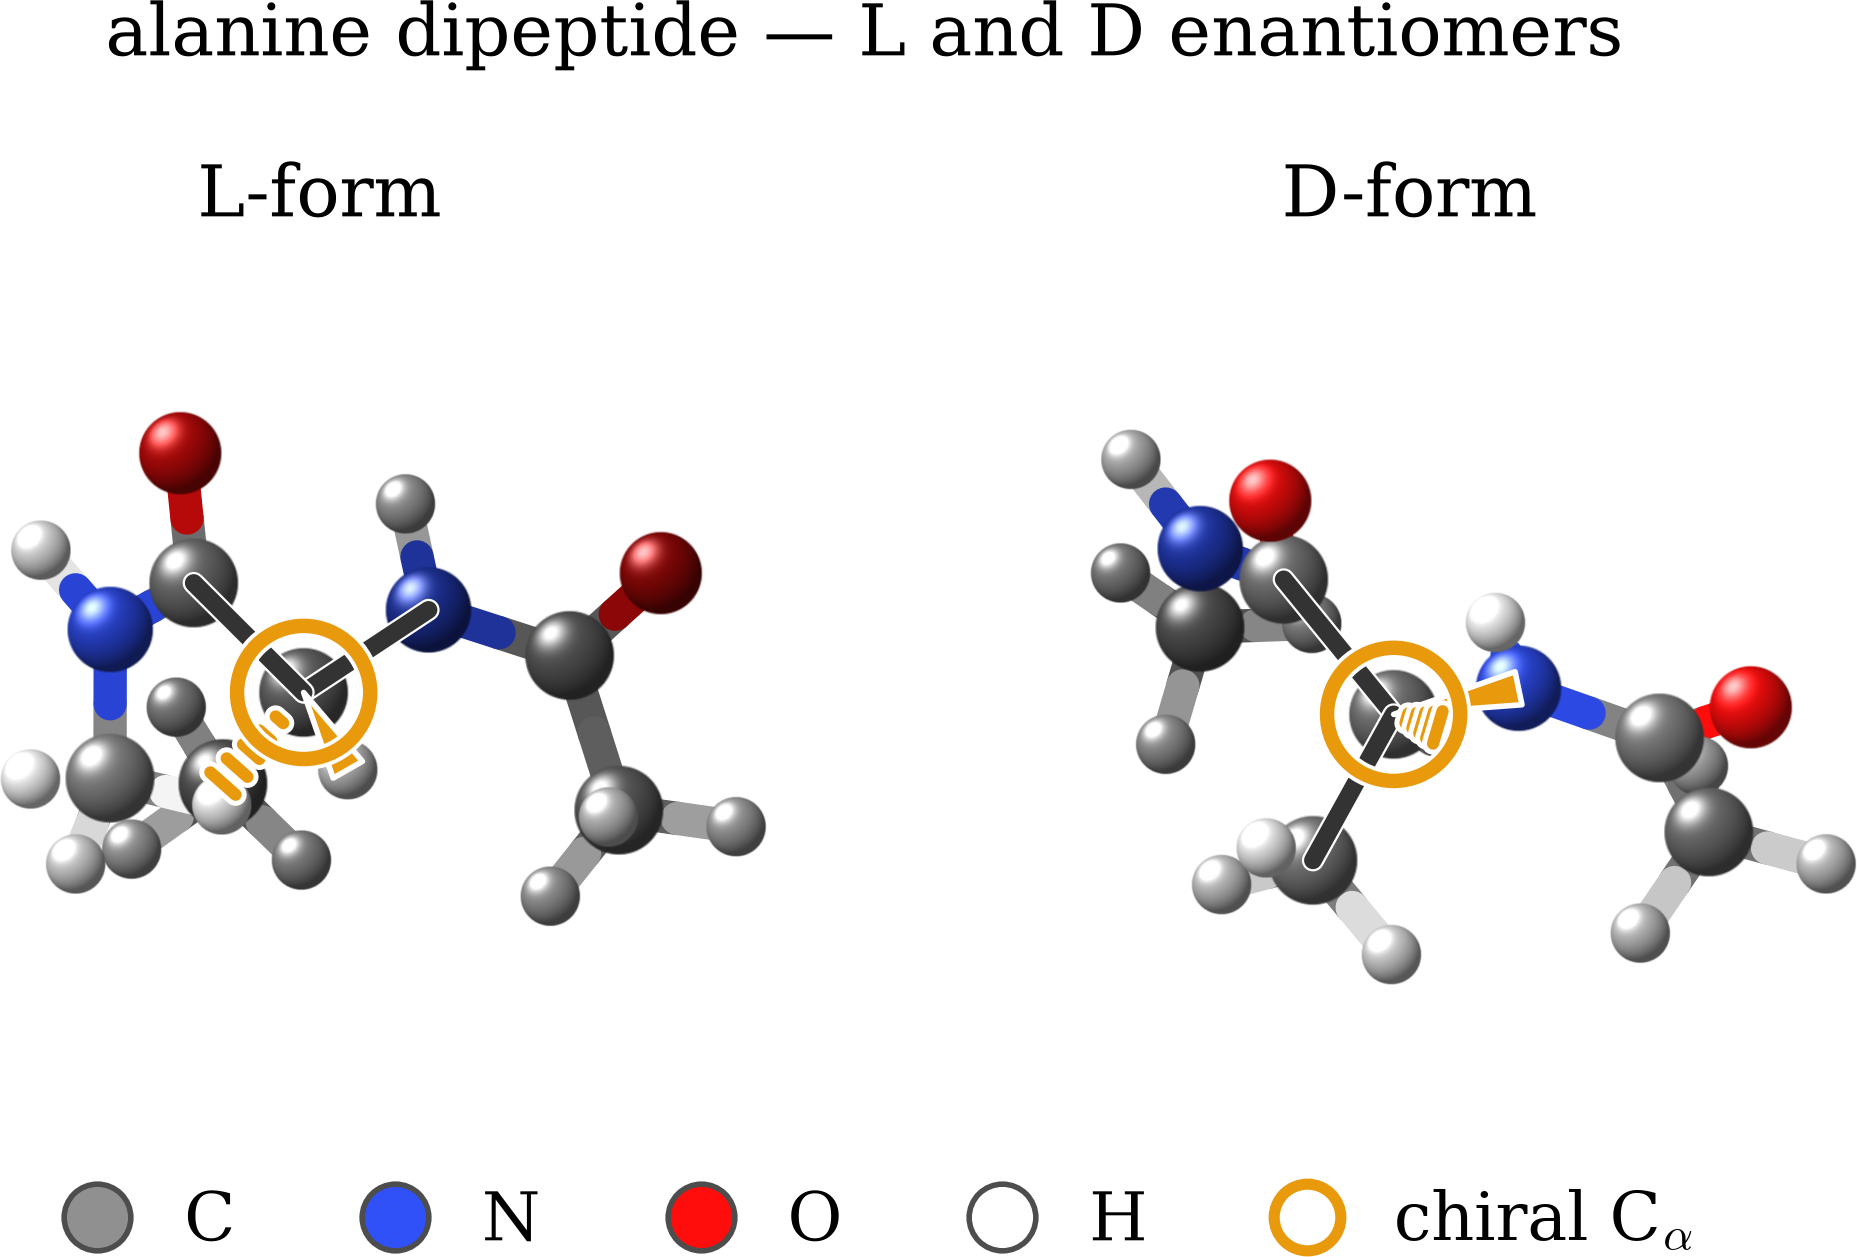
\includegraphics[width=0.6\linewidth]{figures/Molecular_BG/adp_60d/conformers.png}
    \caption{The two enantiomers of alanine dipeptide: the energy-minimized L-form and the D-form, a 3D
    reflection of it, shown from different viewpoints (ball-and-stick; C grey, N blue, O red, H white). The
    chiral $\mathrm{C}_\alpha$ is ringed in gold with stereo bonds, a solid wedge toward the viewer and hashed
    bonds behind. The achiral Amber force field makes the two isoenergetic, so the generator emits both, the
    structural companion to the $(\phi,\psi)\!\to\!(-\phi,-\psi)$ Ramachandran symmetry of
    Figure~\ref{fig: adp-rama}.}
    \label{fig: adp-conformers}
\end{figure}

\begin{figure}[htb]
    \centering
    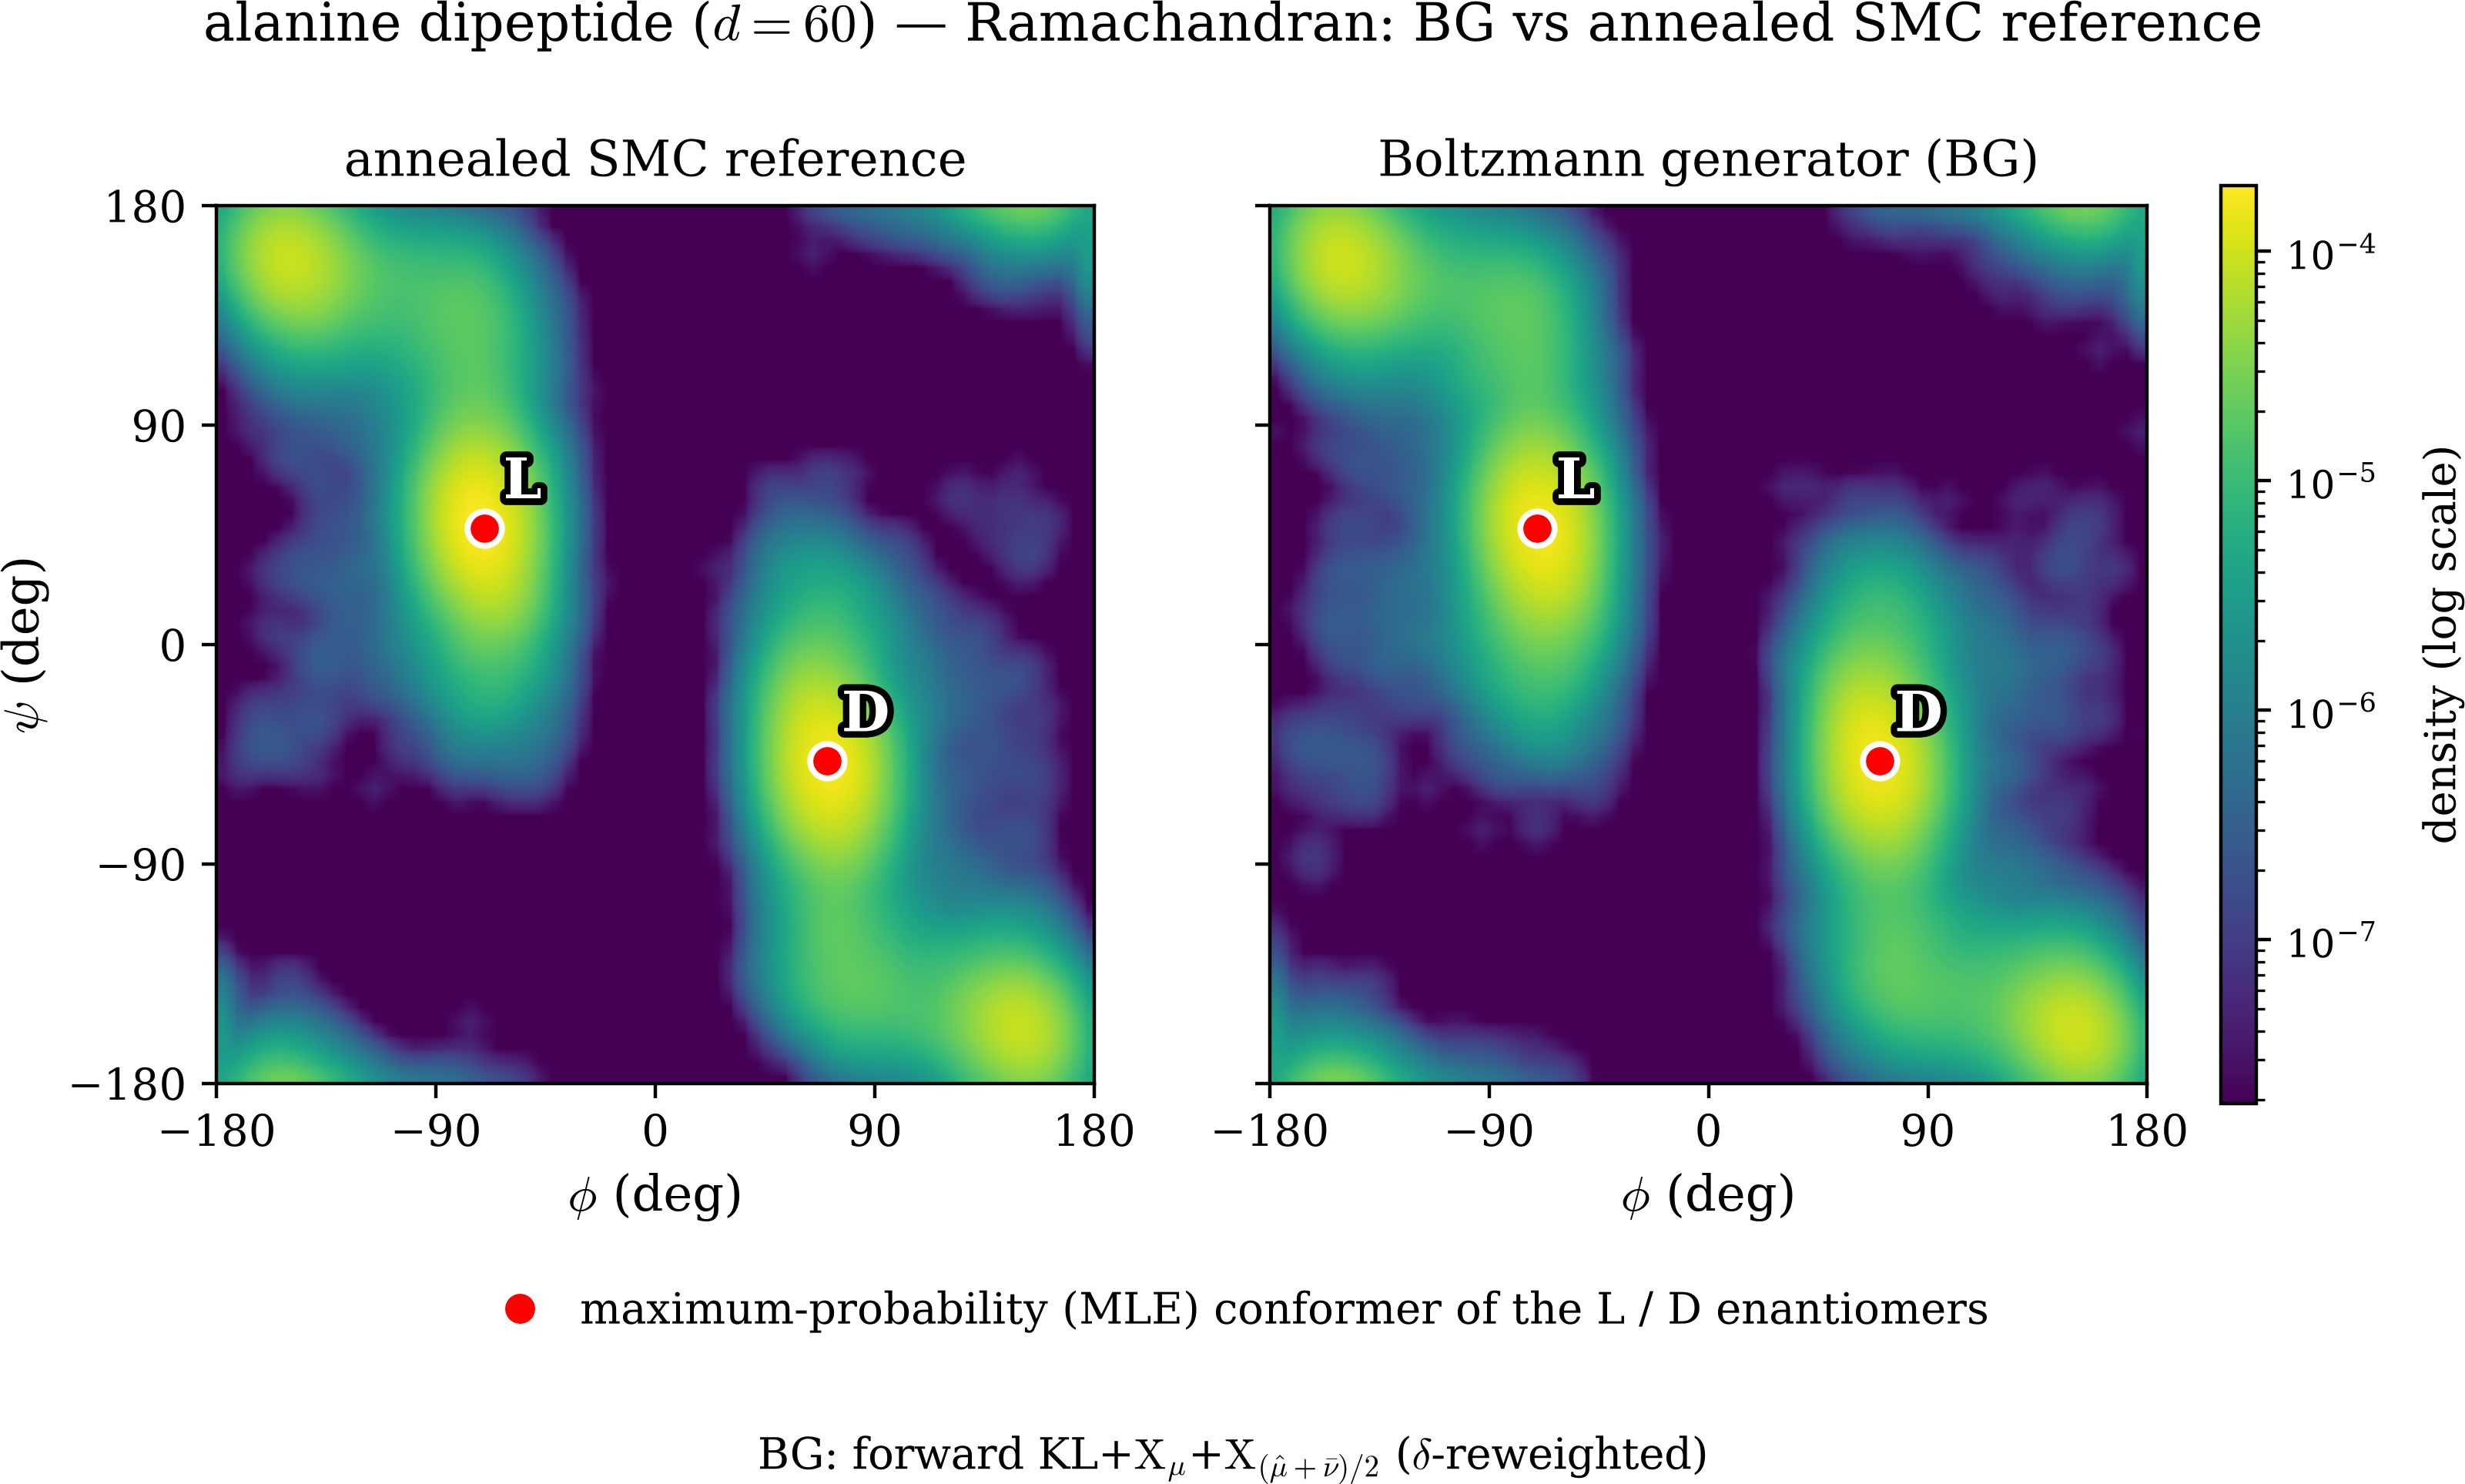
\includegraphics[width=0.92\linewidth]{figures/Molecular_BG/adp_60d/ramachandran.png}
    \caption{Alanine dipeptide Ramachandran ($\phi,\psi$), shared log-density scale: the BG deliverable
    (right) against the annealed SMC reference (left). Red dots mark the maximum-probability conformer of
    each enantiomer (L at $\phi<0,\psi>0$; D at $\phi>0,\psi<0$). Both panels populate the same backbone basins
    with the $(\phi,\psi)\!\to\!(-\phi,-\psi)$ point symmetry: the achiral vacuum force field makes the L- and
    D-enantiomers isoenergetic, and the generator, carrying no chirality constraint, samples both
    (Section~\ref{sec: adp}).}
    \label{fig: adp-rama}
\end{figure}

The X-regularized BG closes the full internal-coordinate alanine dipeptide target to $t = 1$ in $11$ stages at
$F^{*} = 67.95$, recovering the multimodal backbone torsions against a converged annealed SMC reference and emitting both
chiral forms of the mirror-symmetric target. The lesson carried over from the lighter $d \Le 48$ molecules is
inverted: alanine dipeptide's difficulty is not its combinatorial torsion multimodality but its nonbonded clash core,
concentrated in the $t \approx 0.3$--$0.43$ stages, which the particle drop,
best $\ESS$ gate snapshots, and $r$-floor anneal together make tractable. Across all three molecules the
pattern is consistent: the sharpening split makes the singular target trainable at all, and the
X-regularized flow then earns a ${\sim}30$--$40\times$ reduction in importance-weight waste where the landscape is
multimodal but clash-mild, narrowing to ${\sim}2\times$ where the singularity itself dominates.

\subsection{Limitations}
\label{sec: mol-limitations}

Four deliberate simplifications bound the molecular experiments, each a direction for future work. First, the
targets are evaluated in vacuum: $U_{\mathrm{FF}}$ is the isolated-molecule Amber potential \eqref{eq: amber} with no solvent
and no nonbonded cutoff. Solvation only reshapes $U_{\mathrm{FF}}$ and not the sampler, and the vacuum targets already
display the well-separated potential wells the generator must discover and resolve, but implicit or explicit
solvent and larger peptides are left untreated. Second, the internal-coordinate generator carries no chirality
constraint, so for the achiral Amber force field it samples both the L- and D-enantiomers
(Section~\ref{sec: adp}), whereas a physical trajectory stays in one; isolating a single enantiomer by a filter
or restraint is left to future work. Third, we do not benchmark against FAB
\citep{midgley2022flow}: its large per-step batches and replay buffer make a like-for-like comparison under the
same compute budget as these forward KL-type losses prohibitive, so the natural same-cost baselines here are
the bare forward KL and the identity-flow annealed SMC. Fourth, on the alanine dipeptide clash core the
per-stage flow training is unstable and can degenerate toward the identity map, as documented in
Section~\ref{sec: adp}; the best $\ESS$ gate works around this but does not cure it, and a regularization or
parameterization that conditions the repulsive wall remains open.



\bibliographystyle{plainnat}
\bibliography{references}

\end{document}
